% \section{Analisis Masalah dan Kebutuhan Sistem}
% \label{sec:analisis}

% Analisis masalah dilakukan melalui pendekatan kualitatif dengan melakukan wawancara mendalam serta survei lapangan terhadap pemangku kepentingan utama di lingkungan Rusunami The Jarrdin Cihampelas (RTJC).

% % \subsection{Kondisi Faktual Pengelolaan Penyewaan}
% % Berdasarkan wawancara yang dilakukan pada tanggal 27 Maret 2025 dan 13 Oktober 2025 dengan perwakilan agen Paguyuban Komersil Jarrdin (PKJ) dan pengurus P3SRS, teridentifikasi beberapa poin krusial terkait kondisi faktual pengelolaan saat ini:

% % \begin{enumerate}
% %     \item \textbf{Desentralisasi data} \\
% %     Saat ini, setiap agen mengelola data penyewanya masing-masing secara terpisah dan manual. Tidak ada basis data terpusat yang memungkinkan pengelola (P3SRS/PKJ) untuk memantau aktivitas penyewaan secara menyeluruh. Hal ini menyulitkan deteksi dini terhadap penyewa yang berpindah-pindah agen untuk menghindari pelacakan rekam jejak buruk.

% %     \item \textbf{Keterbatasan akses informasi} \\
% %     Agen hanya memiliki visibilitas terhadap data unit yang mereka kelola sendiri. Kebutuhan di lapangan menunjukkan perlunya hierarki akses di mana peran otoritas seperti Ketua Agen, P3SRS, dan PKJ dapat melihat rekapitulasi data dari seluruh agen untuk keperluan pengawasan dan evaluasi mingguan/bulanan.

% %     \item \textbf{Pencatatan yang belum terstandarisasi}\\
% %     Input data masih bervariasi antar agen. Diperlukan standarisasi input yang mencakup NIK, status pernikahan (pasutri/bukan), jenis sewa (harian/bulanan), dan metode pembayaran untuk keperluan analisis deteksi perilaku penyewa.

% %     \item \textbf{Pengawasan manual dan reaktif} \\
% %     Deteksi pelanggaran saat ini bersifat reaktif, sering kali baru diketahui setelah penyewa \textit{check-out} melalui pemeriksaan fisik unit (misalnya temuan alat kontrasepsi atau jarum suntik). Belum ada sistem yang memberikan peringatan dini (\textit{early warning}) berdasarkan pola data administratif saat penyewaan berlangsung.
% % \end{enumerate}


% \subsection{Kondisi Faktual Pengelolaan Penyewaan}

% \begin{figure}[h]
%     \centering
%     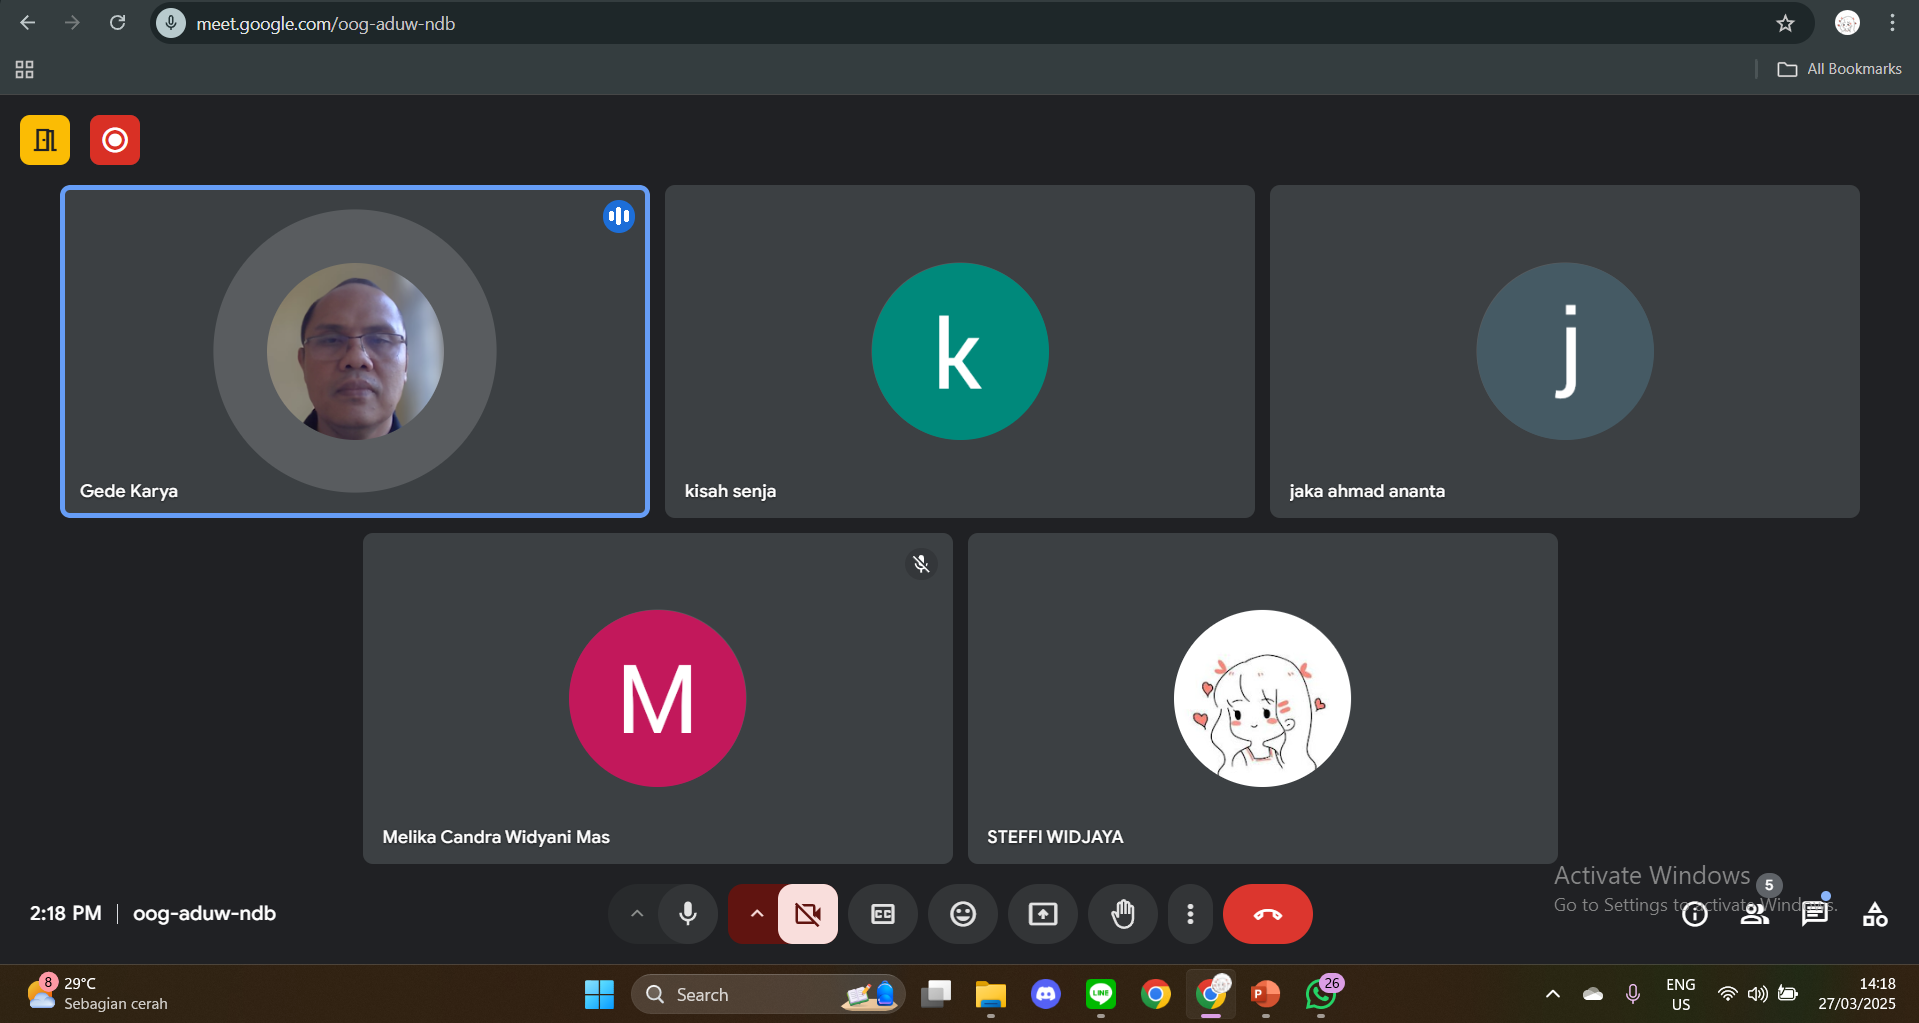
\includegraphics[width=0.45\textwidth]{Gambar/dokumentasi wawancara.png}
%     \caption{Dokumentasi Pertemuan Wawancara dengan Narasumber secara {\it Online}}
%     \label{fig:wawancara_online}
% \end{figure}

% % Berdasarkan rangkaian kegiatan yang telah dilakukan, meliputi wawancara murni pada tanggal 23 Maret 2025 (melalui Google Meet), wawancara dan survei untuk mendapatkan kebutuhan pihak RTJC pada tanggal 31 Mei 2025 (secara langsung di The Jarrdin), serta konfirmasi sistem dan jaring masukan dari para narasumber pada tanggal 13 Oktober 2025 (secara langsung di The Jarrdin) bersama perwakilan agen Paguyuban Komersil Jarrdin (PKJ) dan pengurus P3SRS (Bapak Rey, Bapak Jaka, dan Bapak Diki), teridentifikasi beberapa kondisi faktual dan poin krusial terkait pengelolaan saat ini sebagai berikut.
% Berdasarkan rangkaian kegiatan pengumpulan data yang telah dilakukan (sejalan dengan karakteristik pengelolaan dan dinamika penghuni sebagaimana dijelaskan pada kajian teori terkait rumah susun di Subbab~\ref{sec:rumah_susun})—meliputi wawancara awal pada tanggal 23 Maret 2025 (secara daring melalui Google Meet), wawancara dan survei lapangan untuk pemetaan kebutuhan pada tanggal 31 Mei 2025 (di lokasi Apartemen The Jarrdin), serta sesi konfirmasi purwarupa sistem dan penjaringan masukan pada tanggal 13 Oktober 2025 (di lokasi Apartemen The Jarrdin)—bersama dengan pihak pengelola yang terdiri dari perwakilan agen Paguyuban Komersil Jarrdin (PKJ) serta pengurus Perhimpunan Pemilik dan Penghuni Satuan Rumah Susun (P3SRS) (Bapak Rey, Bapak Jaka, dan Bapak Diki), teridentifikasi beberapa kondisi faktual dan poin krusial terkait tata kelola saat ini sebagai berikut.

% \begin{enumerate}
%     \item \textbf{Desentralisasi data dan pengelolaan manual} \\
%     Saat ini, sistem penyewaan unit dikelola secara terpisah dan manual tanpa bantuan sistem teknologi terintegrasi. Tidak ada basis data terpusat yang memungkinkan pengelola untuk memantau aktivitas penyewaan secara menyeluruh. 
%     \begin{itemize}
%         \item Data penyewaan belum tersimpan dalam sistem digital yang terstruktur, melainkan dikelola masing-masing oleh agen.
%         \item Ketidakhadiran data historis yang terdokumentasi dengan baik menyulitkan deteksi dini terhadap penyewa yang berpindah-pindah agen untuk menghindari pelacakan rekam jejak buruk.
%     \end{itemize}

%     \item \textbf{Keterbatasan akses informasi dan hierarki} \\
%     Agen hanya memiliki visibilitas terhadap data unit yang mereka kelola sendiri. Kebutuhan di lapangan menunjukkan perlunya hierarki akses di mana peran otoritas seperti Ketua Agen, P3SRS, dan PKJ dapat melihat rekapitulasi data dari seluruh agen untuk keperluan pengawasan dan evaluasi. Saat ini, belum ada sistem \textit{data capture} yang memungkinkan penarikan data dari agen atau penyewa untuk kebutuhan ini.

%     \item \textbf{Standarisasi pencatatan dan administrasi} \\
%     Input data masih bervariasi antar agen. Meskipun penyewa dan pemilik unit diwajibkan menandatangani surat perjanjian sewa untuk menghindari risiko kriminal dan kelalaian, data transaksi tersebut belum dimanfaatkan untuk analisis. Diperlukan standarisasi input digital yang mencakup hal berikut.
%     \begin{itemize}
%         \item Identitas penyewa (NIK) dan agen penanggung jawab.
%         \item Unit kamar yang disewa.
%         \item Status kewarganegaraan penyewa.
%         \item Status pernikahan (pasutri/bukan) dan metode pembayaran.
%         \item Waktu \textit{check-in/check-out} serta durasi menginap (harian/bulanan).
%     \end{itemize}
%     Data-data ini divalidasi oleh narasumber sebagai variabel yang sangat memungkinkan untuk dikumpulkan dan krusial untuk keperluan analisis perilaku.

%     \item \textbf{Pengawasan manual dan pola deteksi reaktif} \\
%     Saat ini belum ada sistem peringatan dini (\textit{early warning}) berbasis pola data administratif. Fakta lapangan menunjukkan:
%     \begin{itemize}
%         \item pelanggaran sering kali baru diketahui setelah penyewa menginap lebih dari dua hari, saat layanan kebersihan (\textit{cleaning service}) menemukan barang mencurigakan di tempat sampah (seperti alat kontrasepsi atau jarum suntik dalam jumlah tidak wajar),
%         \item kasus yang paling sering terjadi adalah praktik prostitusi dan penyalahgunaan narkoba,
%         \item tidak ada pola visual (gaya berpakaian/penampilan) yang dapat dijadikan acuan. Pelanggaran dapat dilakukan oleh individu maupun kelompok, serta terjadi pada penyewa harian (transit/liburan) maupun bulanan.
%         \item saat penyewa bermasalah ditemukan, belum ada dokumentasi formal mengenai proses penyelesaian masalah tersebut, sehingga pola pelanggaran sulit dipelajari secara historis.
%     \end{itemize}
% \end{enumerate}


%         \begin{figure}[H]
%             \centering
%             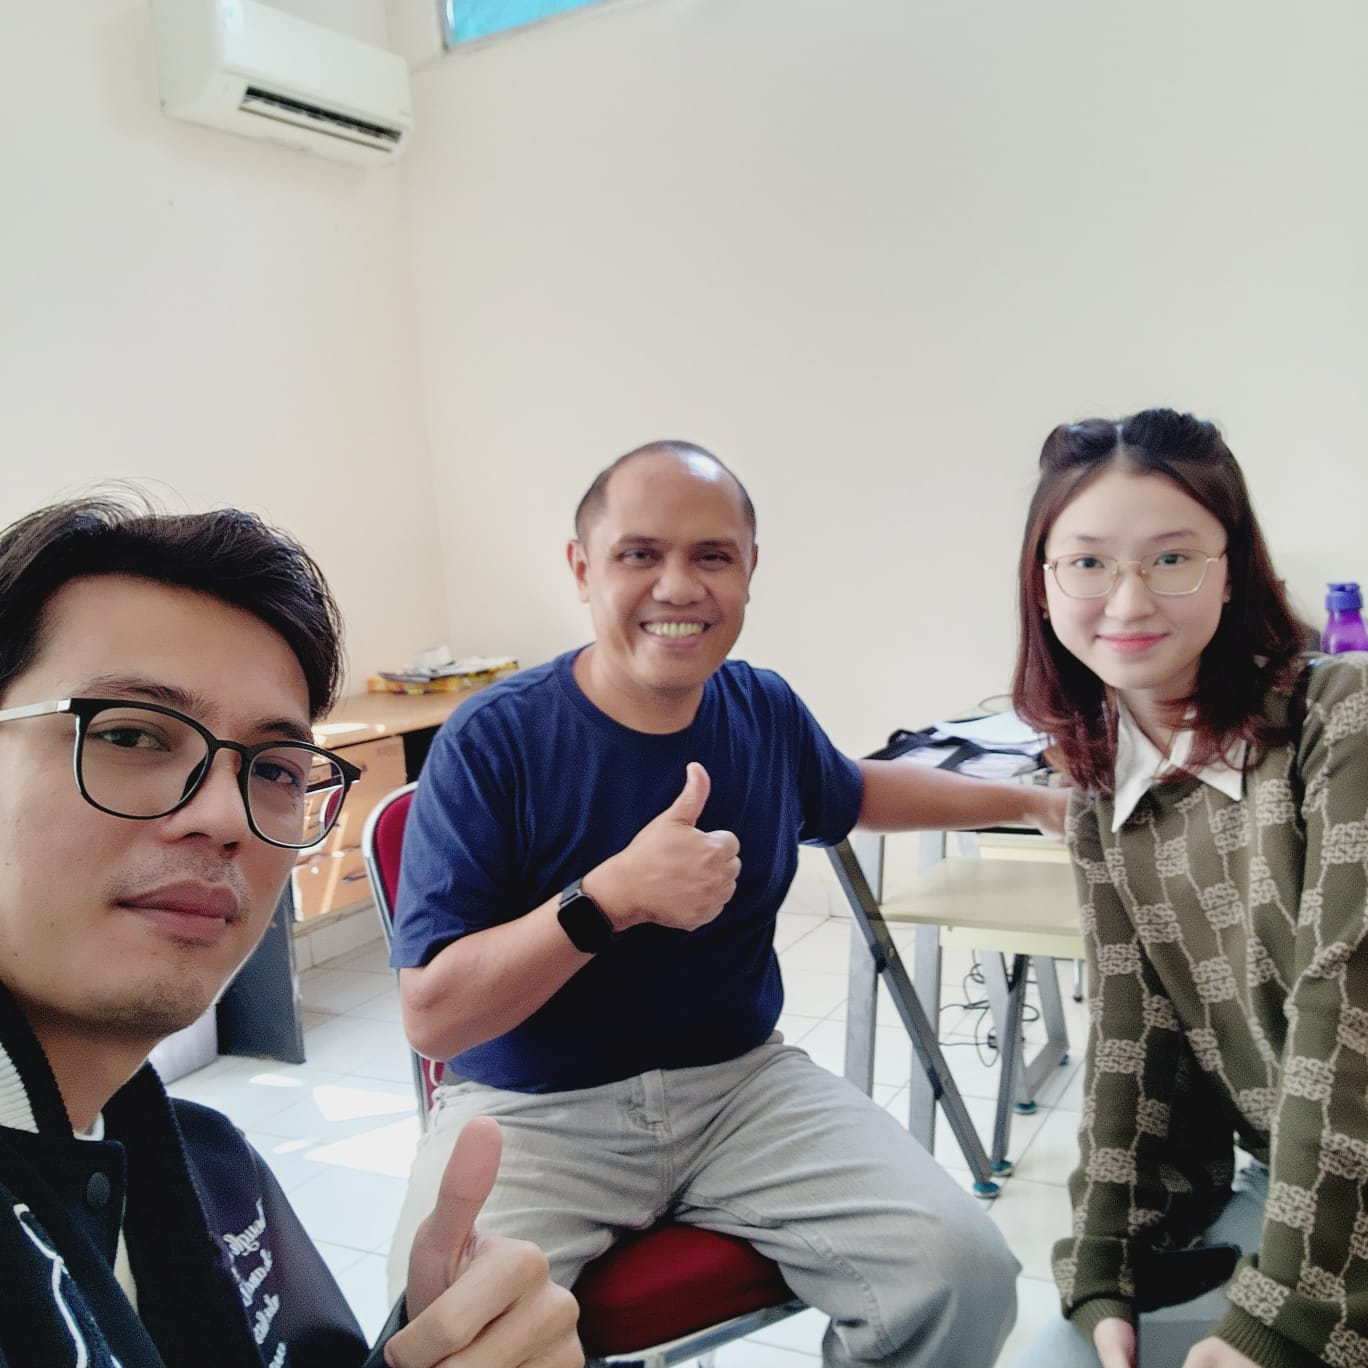
\includegraphics[width=0.5\textwidth, max height=0.4\textheight]{Gambar/dokumentasi wawancara2.jpg}
%             \caption{Dokumentasi Pertemuan Wawancara dengan Narasumber secara {\it Offline}}
%             \label{fig:dokumentasi wawancara2}
%         \end{figure}


% \newpage
% Selain wawancara daring, survei lapangan juga dilaksanakan guna mendata kondisi fisik dan fasilitas yang ada. Melalui kegiatan ini, diperoleh pula berbagai informasi mengenai sistem sewa, fasilitas, serta struktur pengelolaan di kawasan hunian tersebut. The Jarrdin memiliki total sekitar 2.400 unit yang terbagi ke dalam beberapa tipe, yakni tipe studio (18~m\textsuperscript{2} dan 24~m\textsuperscript{2}) serta tipe dua kamar (33~m\textsuperscript{2} dan 40~m\textsuperscript{2}). Unit tipe studio terdiri atas satu ruangan multifungsi yang menggabungkan area tidur, dapur, dan ruang tamu; sedangkan tipe dua kamar memiliki pemisahan ruang yang lebih tegas, mencakup kamar tidur terpisah, dapur, serta ruang tamu.

% \vspace{0.5cm} Sistem penyewaan unit menerapkan skema       ``titip sewa'' kepada agen. Dalam skema ini, pemilik unit menyerahkan pengelolaan kepada agen dengan kesepakatan nilai kontrak bulanan yang tetap, terlepas dari apakah unit tersebut berhasil disewakan atau tidak. Bapak Diki Andrian Permana, salah satu agen yang diwawancarai, menjelaskan bahwa segala permasalahan yang dialami penyewa akan diarahkan terlebih dahulu kepada tim \textit{Tenant Relation} (TR) untuk penanganan awal. Syarat penitipan unit mengharuskan pemilik menyerahkan sejumlah dokumen, antara lain KTP pemilik dan agen, PPJB (Perjanjian Pengikatan Jual Beli), serta surat perjanjian sewa-menyewa.

% \vspace{0.5cm} Kawasan The Jarrdin terdiri atas empat tower dengan identitas warna yang berbeda, yakni Tower A (kuning), Tower B (hijau), Tower C (biru), dan Tower D (oranye). Fasilitas yang tersedia terbilang lengkap, meliputi kolam renang, akses langsung ke Cihampelas Walk (Ciwalk), area parkir basement, lift, ruang tunggu, supermarket, masjid, dan gereja GBI. Selain itu, terdapat area parkir darurat di lantai B2 yang difungsikan sebagai titik penanganan awal apabila terjadi pelanggaran atau situasi darurat. Terkait durasi sewa, unit dapat disewakan secara harian hingga mingguan. Pada sewa harian, biaya IPL (Iuran Pemeliharaan Lingkungan) dan token listrik ditanggung oleh penyewa, sedangkan untuk sewa bulanan, biaya tersebut menjadi tanggung jawab pemilik unit.

% \vspace{0.5cm} Pengelolaan Rusunami dijalankan oleh pengurus di bawah pengawasan P3SRS (Perhimpunan Pemilik dan Penghuni Satuan Rumah Susun), yang anggotanya terdiri dari para pemilik unit sesuai ketentuan AD/ART. Struktur kepengurusan mencatat beberapa nama, antara lain Bapak Fendy Efendi (Ketua), Rudi Wiranata Kusumah (Sekretaris), serta Dewi Juwita dan Cici Pricillia Susanto (Bendahara). Bidang operasional diisi oleh Bapak Jaka (Kepenghunian) dan Bapak Rey (Pengelolaan), sementara fungsi pengawasan dijalankan oleh Bapak Agus Anwar, Bapak Erwin, dan Bapak Gede. Di sisi lain, aspek komersial dikelola oleh komunitas PKJ (Paguyuban Komersil Jarrdin) yang dipimpin oleh Bapak Hans, dibantu oleh Bapak Diki selaku sekretaris dan Ibu Marliana Furey sebagai bendahara.

% \vspace{0.5cm} Tarif parkir di kawasan ini telah ditetapkan sebesar Rp25.000,00 per hari untuk mobil dan Rp15.000,00 untuk motor. Bagi penghuni yang berlangganan bulanan, biaya parkir motor dikenakan Rp75.000,00 dan mobil sebesar Rp150.000,00. Mengenai penanganan ketertiban, penghuni atau penyewa yang melakukan pelanggaran akan diarahkan ke area B2 untuk ditindaklanjuti oleh pengelola, dengan melibatkan orang tua, agen, atau pihak kepolisian jika diperlukan. Berikut terlampir dokumentasi visual yang mencakup foto unit setiap tipe, tampilan depan ruang agen, serta berbagai fasilitas yang tersedia di kawasan The Jarrdin.
        
%         \newpage
%         % \begin{figure}[H]
%         %     \centering
%         %     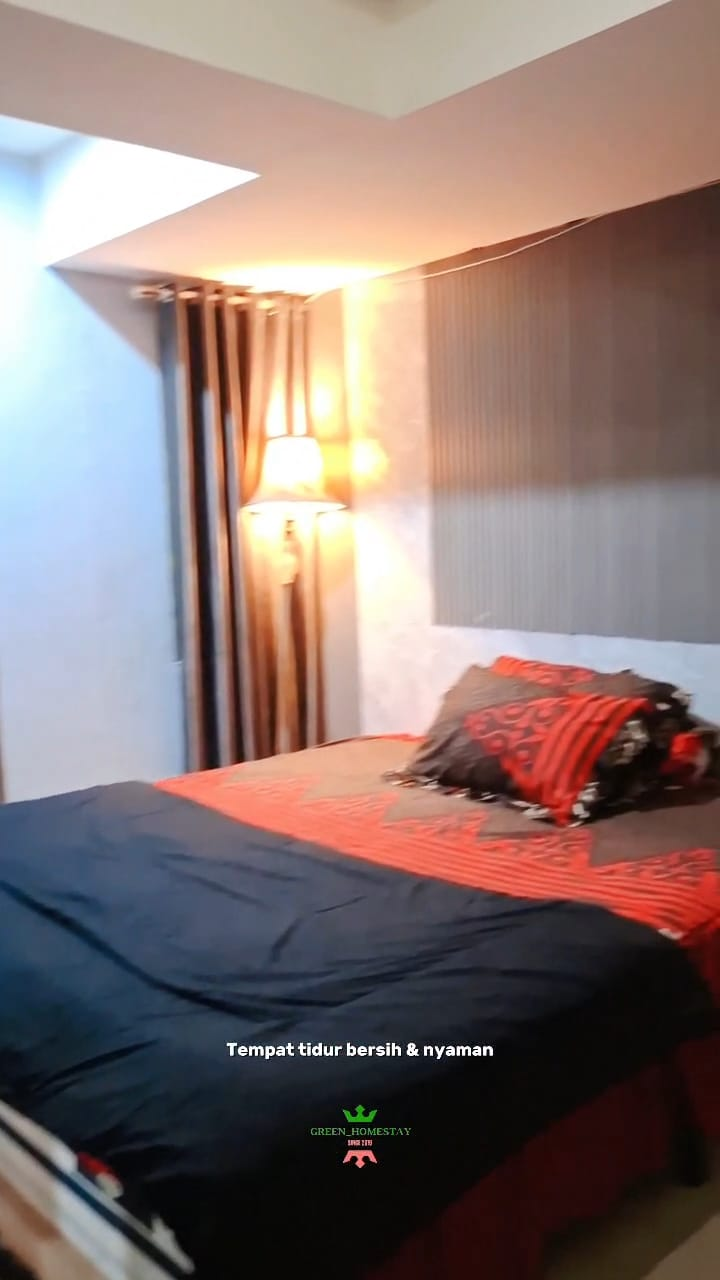
\includegraphics[width=0.5\textwidth, max height=0.45\textheight]{Gambar/tempat tidur - studio.jpg}
%         %     \caption{Contoh Kamar Tidur untuk Tipe Studio}
%         %     \label{fig:tempat tidur - studio}
%         % \end{figure}

%         % \begin{figure}[H]
%         %     \centering
%         %     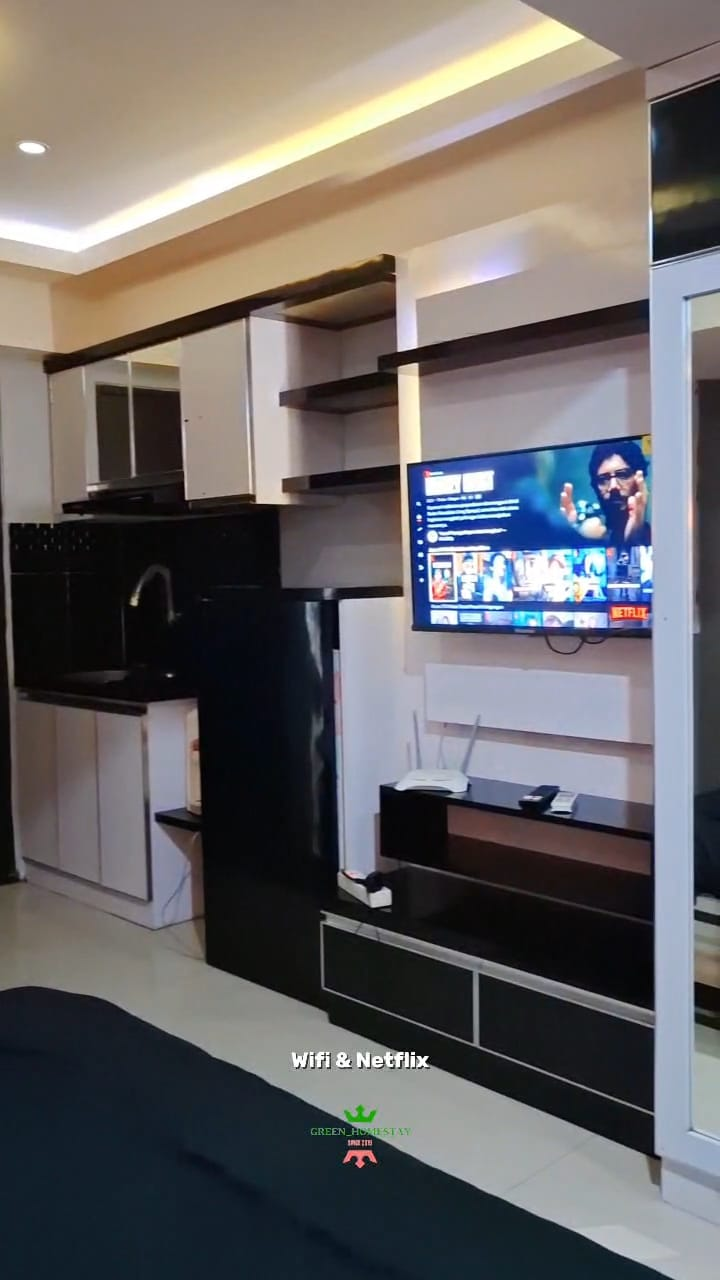
\includegraphics[width=0.5\textwidth, max height=0.45\textheight]{Gambar/ruang tamu - studio.jpg}
%         %     \caption{Contoh Ruang Tamu untuk Tipe Studio}
%         %     \label{fig:ruang tamu - studio}
%         % \end{figure}

%         % \begin{figure}[H]
%         %     \centering
%         %     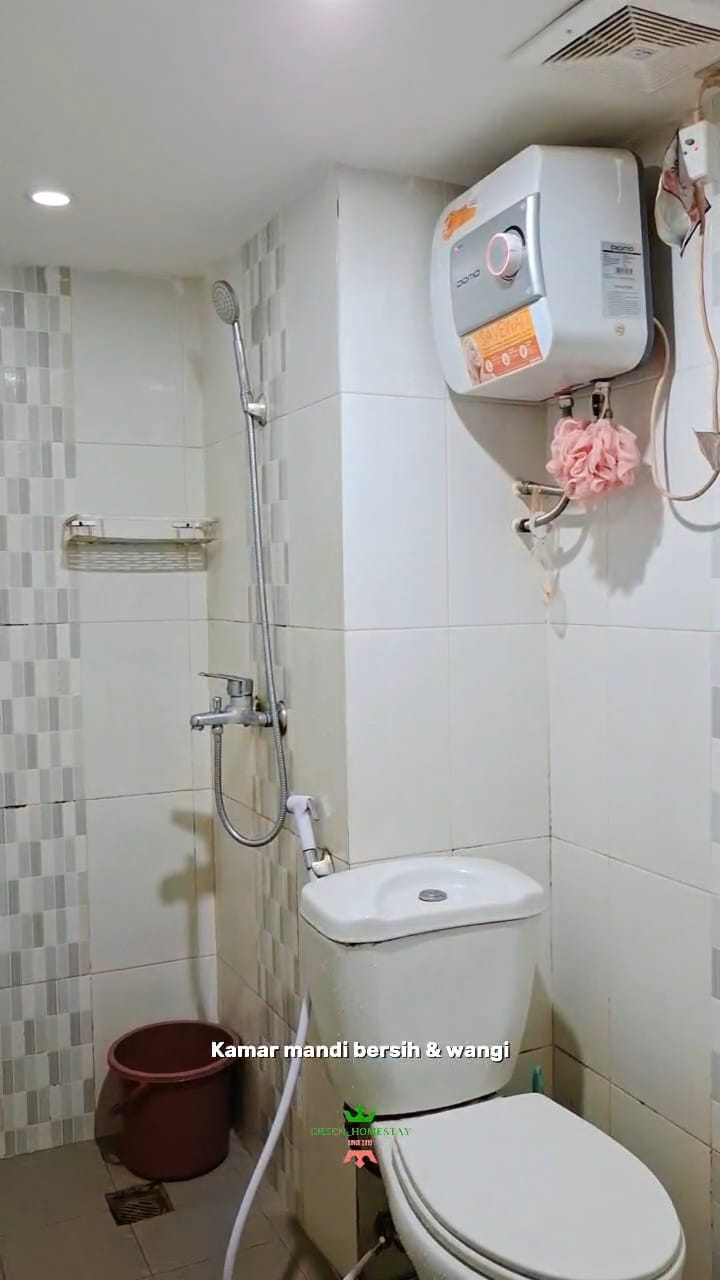
\includegraphics[width=0.5\textwidth, max height=0.45\textheight]{Gambar/kamar mandi - studio.jpg}
%         %     \caption{Contoh Kamar Mandi untuk Tipe Studio}
%         %     \label{fig:kamar mandi - studio}
%         % \end{figure}

%         % \begin{figure}[H]
%         %     \centering
%         %     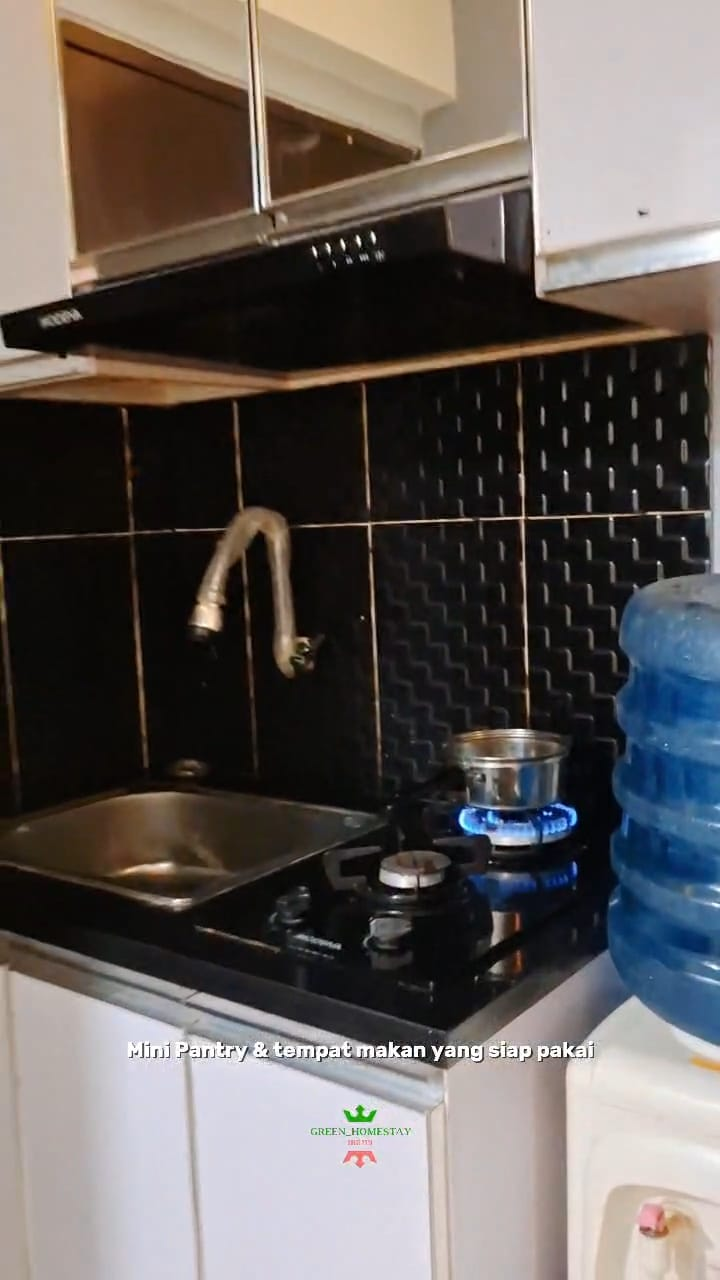
\includegraphics[width=0.5\textwidth, max height=0.45\textheight]{Gambar/dapur - studio.jpg}
%         %     \caption{Contoh Dapur untuk Tipe Studio}
%         %     \label{fig:dapur - studio}
%         % \end{figure}

        
%         % \begin{figure}[H]
%         %     \centering
%         %     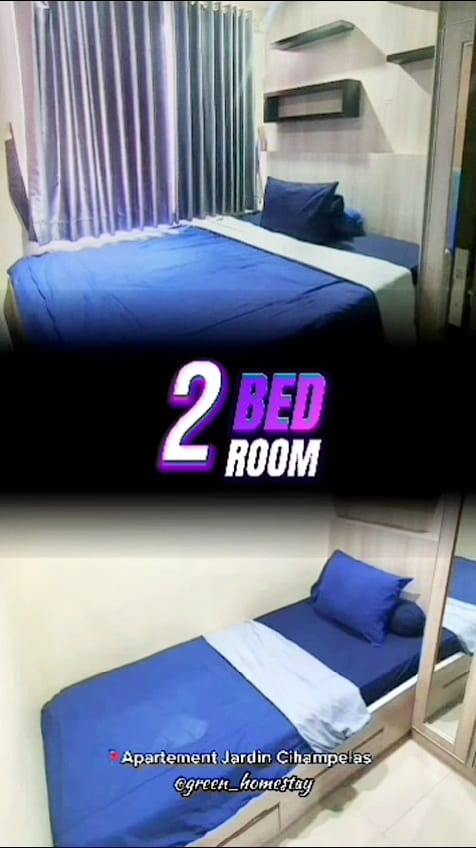
\includegraphics[width=0.5\textwidth, max height=0.45\textheight]{Gambar/kamar - 2 kamar.jpg}
%         %     \caption{Contoh Kamar Tidur untuk Tipe 2 Kamar}
%         %     \label{fig:tempat tidur - 2 kamar}
%         % \end{figure}

%         % \begin{figure}[H]
%         %     \centering
%         %     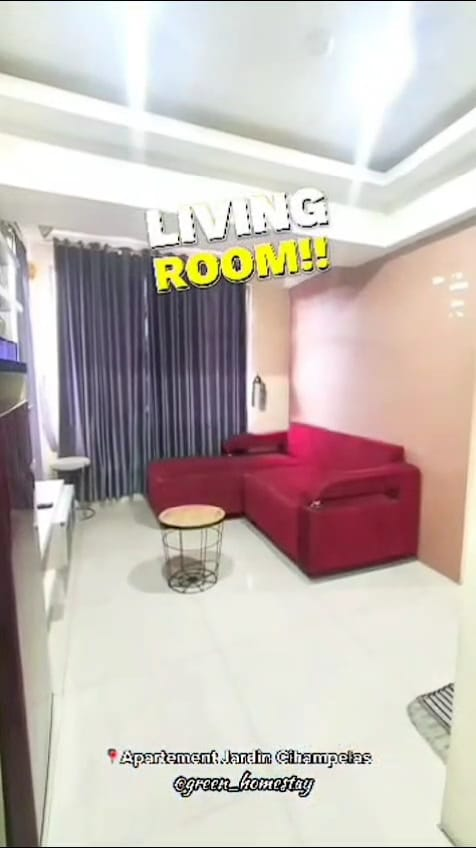
\includegraphics[width=0.5\textwidth, max height=0.45\textheight]{Gambar/ruang tamu - 2 kamar.jpg}
%         %     \caption{Contoh Ruang Tamu untuk Tipe 2 Kamar}
%         %     \label{fig:ruang tamu - 2 kamar}
%         % \end{figure}

%         % \begin{figure}[H]
%         %     \centering
%         %     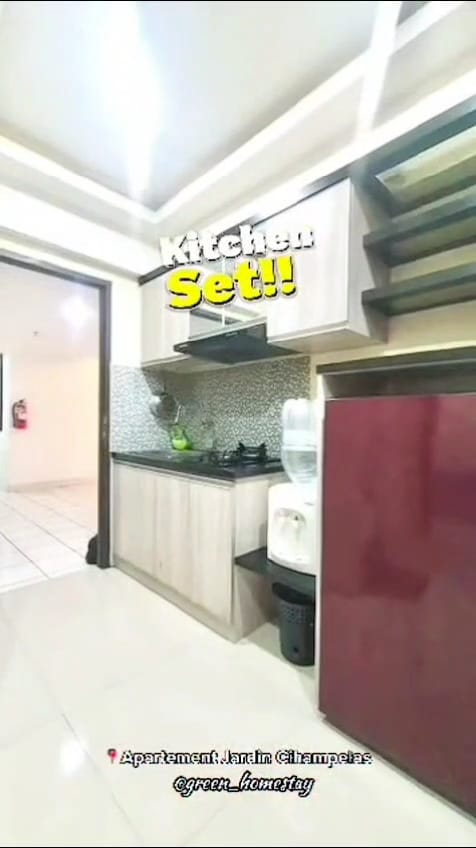
\includegraphics[width=0.5\textwidth, max height=0.45\textheight]{Gambar/dapur - 2 kamar.jpg}
%         %     \caption{Contoh Dapur untuk Tipe 2 Kamar}
%         %     \label{fig:dapur - 2 kamar}
%         % \end{figure}

%         % \begin{figure}[H]
%         %     \centering
%         %     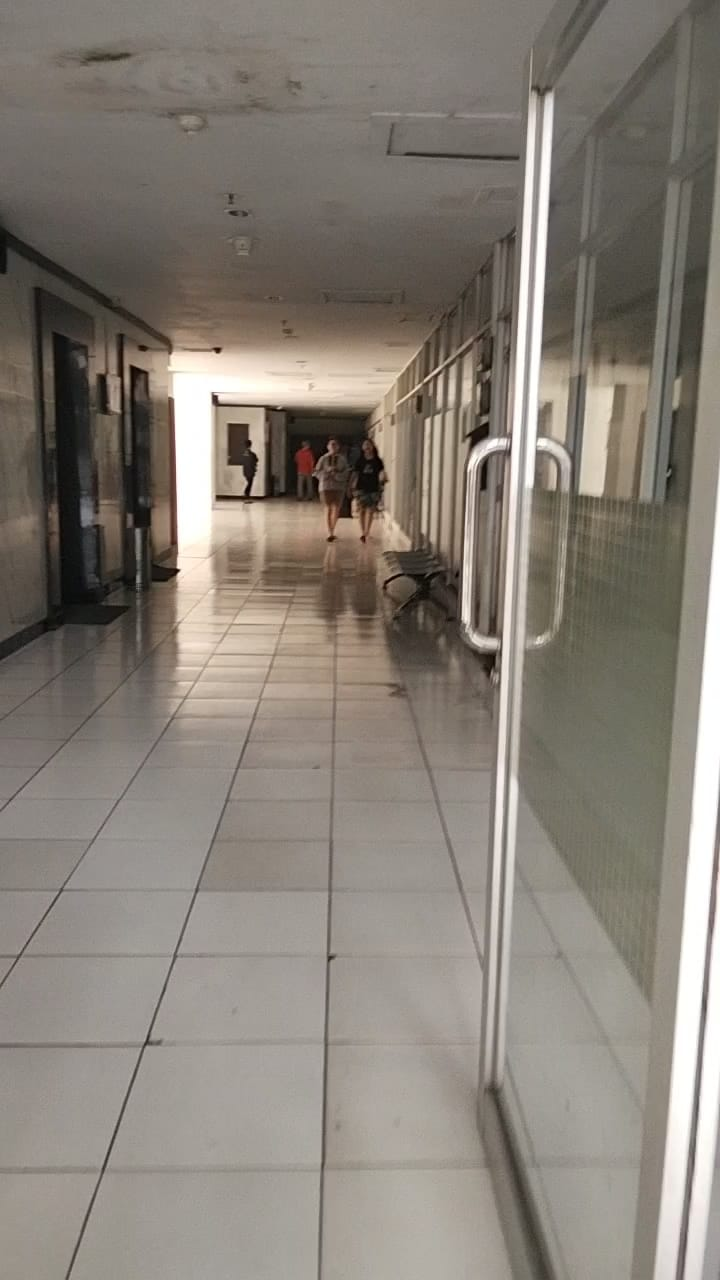
\includegraphics[width=0.5\textwidth, max height=0.45\textheight]{Gambar/tampak depan ruangan2 agen.jpg}
%         %     \caption{Lorong Tempat Ruangan Para Agen}
%         %     \label{fig:tampak depan ruangan2 agen}
%         % \end{figure}


%         % --- GRUP 1: TIPE STUDIO (2x2) ---
%         \begin{figure}[H]
%             \centering
%             % Baris 1, Gambar 1 (Kiri)
%             \begin{minipage}[t]{0.48\textwidth}
%                 \centering
%                 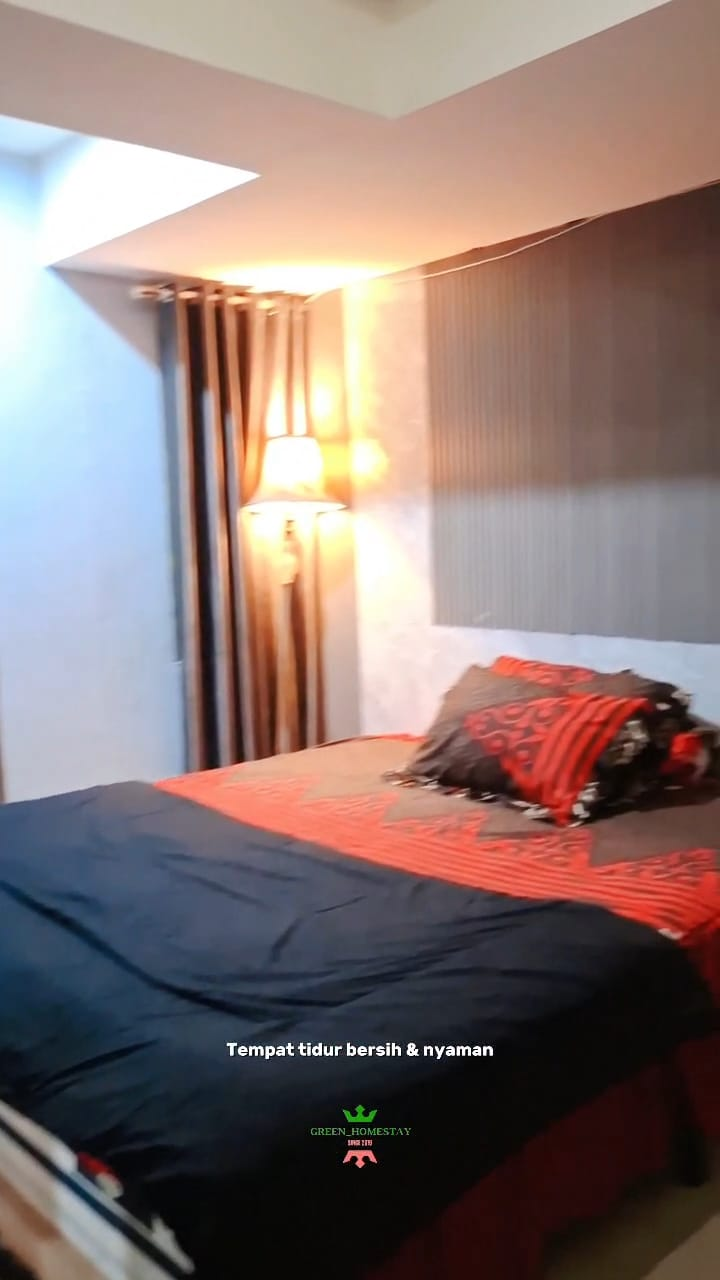
\includegraphics[width=\linewidth, max height=0.45\textheight]{Gambar/tempat tidur - studio.jpg}
%                 \caption{Contoh Kamar Tidur untuk Tipe Studio}
%                 \label{fig:tempat tidur - studio}
%             \end{minipage}
%             \hfill
%             % Baris 1, Gambar 2 (Kanan)
%             \begin{minipage}[t]{0.48\textwidth}
%                 \centering
%                 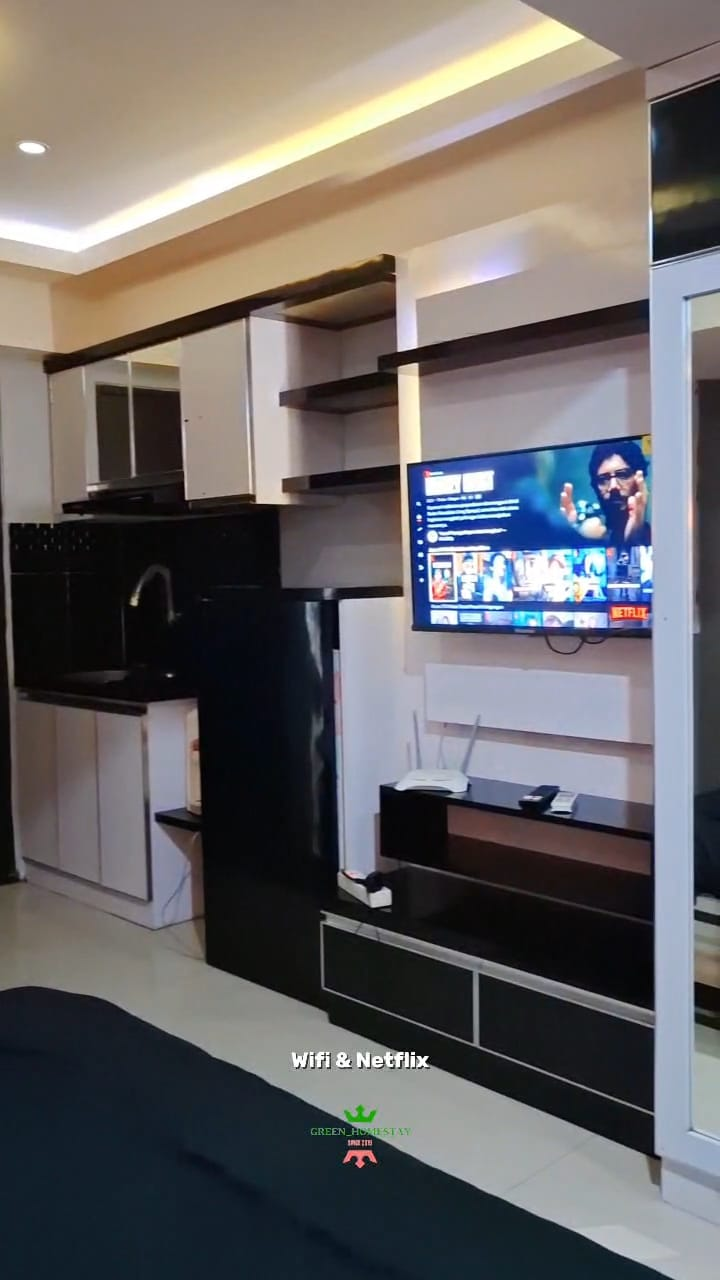
\includegraphics[width=\linewidth, max height=0.45\textheight]{Gambar/ruang tamu - studio.jpg}
%                 \caption{Contoh Ruang Tamu untuk Tipe Studio}
%                 \label{fig:ruang tamu - studio}
%             \end{minipage}
        
%             \vspace{1cm} % Jarak antar baris
        
%             % Baris 2, Gambar 3 (Kiri)
%             \begin{minipage}[t]{0.48\textwidth}
%                 \centering
%                 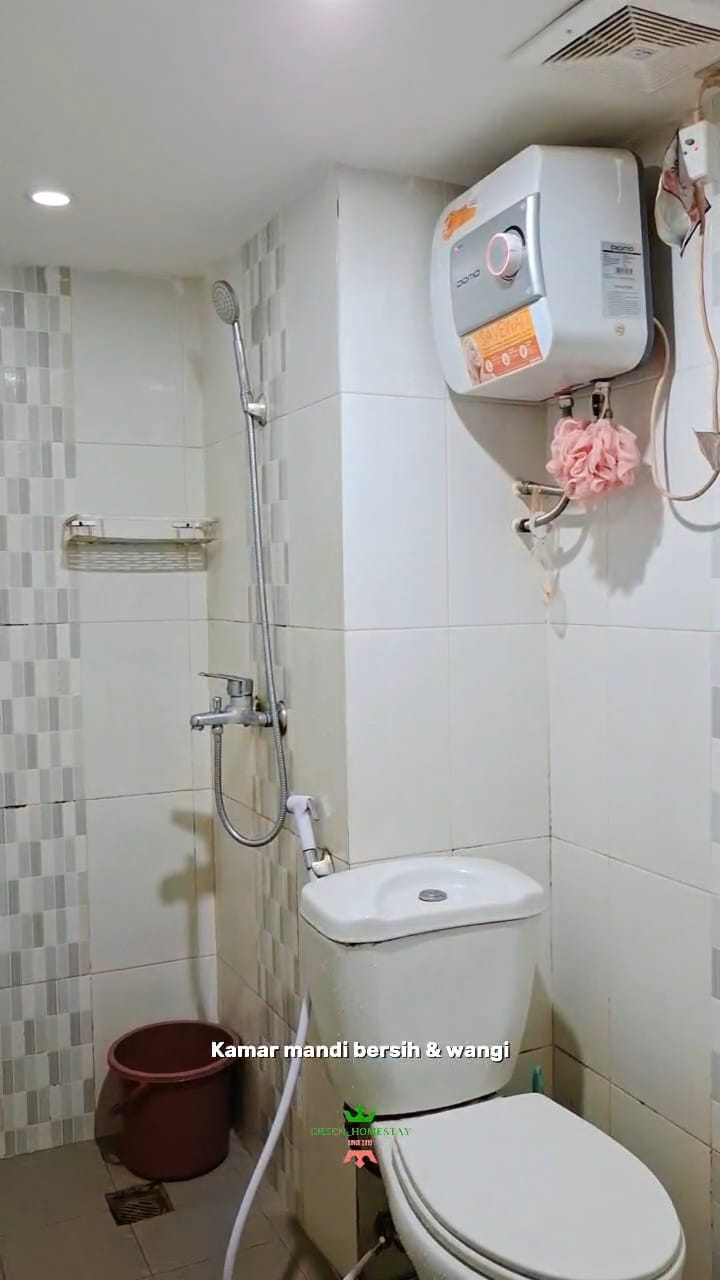
\includegraphics[width=\linewidth, max height=0.45\textheight]{Gambar/kamar mandi - studio.jpg}
%                 \caption{Contoh Kamar Mandi untuk Tipe Studio}
%                 \label{fig:kamar mandi - studio}
%             \end{minipage}
%             \hfill
%             % Baris 2, Gambar 4 (Kanan)
%             \begin{minipage}[t]{0.48\textwidth}
%                 \centering
%                 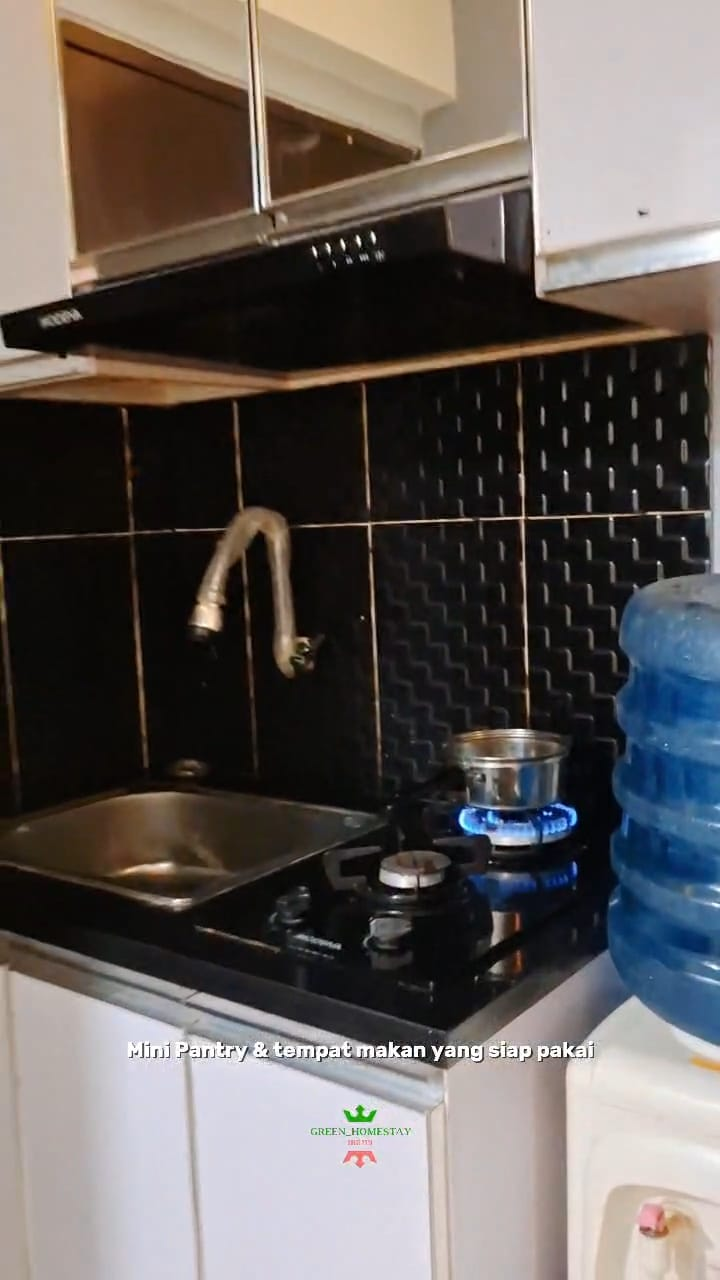
\includegraphics[width=\linewidth, max height=0.45\textheight]{Gambar/dapur - studio.jpg}
%                 \caption{Contoh Dapur untuk Tipe Studio}
%                 \label{fig:dapur - studio}
%             \end{minipage}
%         \end{figure}
        
%         % --- GRUP 2: TIPE 2 KAMAR & AGEN (2x2) ---
%         \begin{figure}[H]
%             \centering
%             % Baris 1, Gambar 1 (Kiri)
%             \begin{minipage}[t]{0.48\textwidth}
%                 \centering
%                 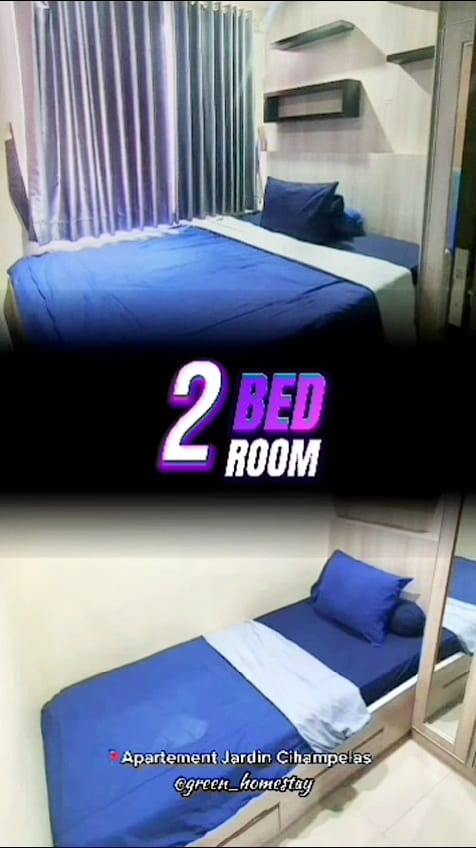
\includegraphics[width=\linewidth, max height=0.45\textheight]{Gambar/kamar - 2 kamar.jpg}
%                 \caption{Contoh Kamar Tidur untuk Tipe 2 Kamar}
%                 \label{fig:tempat tidur - 2 kamar}
%             \end{minipage}
%             \hfill
%             % Baris 1, Gambar 2 (Kanan)
%             \begin{minipage}[t]{0.48\textwidth}
%                 \centering
%                 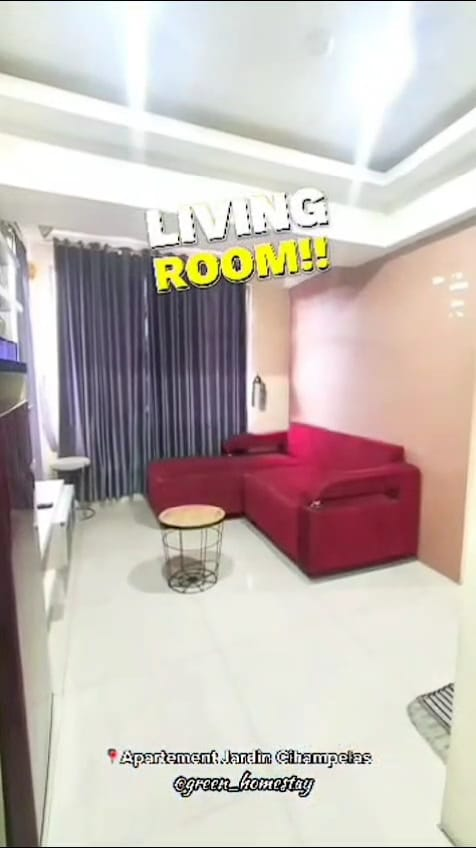
\includegraphics[width=\linewidth, max height=0.45\textheight]{Gambar/ruang tamu - 2 kamar.jpg}
%                 \caption{Contoh Ruang Tamu untuk Tipe 2 Kamar}
%                 \label{fig:ruang tamu - 2 kamar}
%             \end{minipage}
        
%             \vspace{1cm} % Jarak antar baris
        
%             % Baris 2, Gambar 3 (Kiri)
%             \begin{minipage}[t]{0.48\textwidth}
%                 \centering
%                 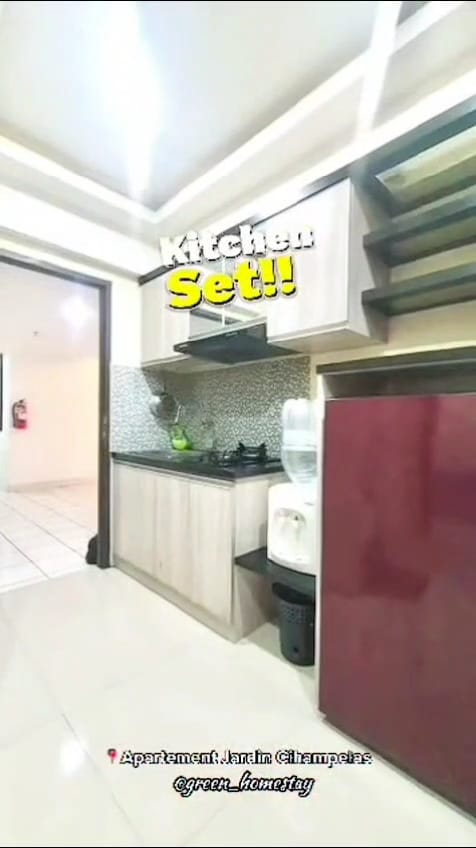
\includegraphics[width=\linewidth, max height=0.45\textheight]{Gambar/dapur - 2 kamar.jpg}
%                 \caption{Contoh Dapur untuk Tipe 2 Kamar}
%                 \label{fig:dapur - 2 kamar}
%             \end{minipage}
%             \hfill
%             % Baris 2, Gambar 4 (Kanan)
%             \begin{minipage}[t]{0.48\textwidth}
%                 \centering
%                 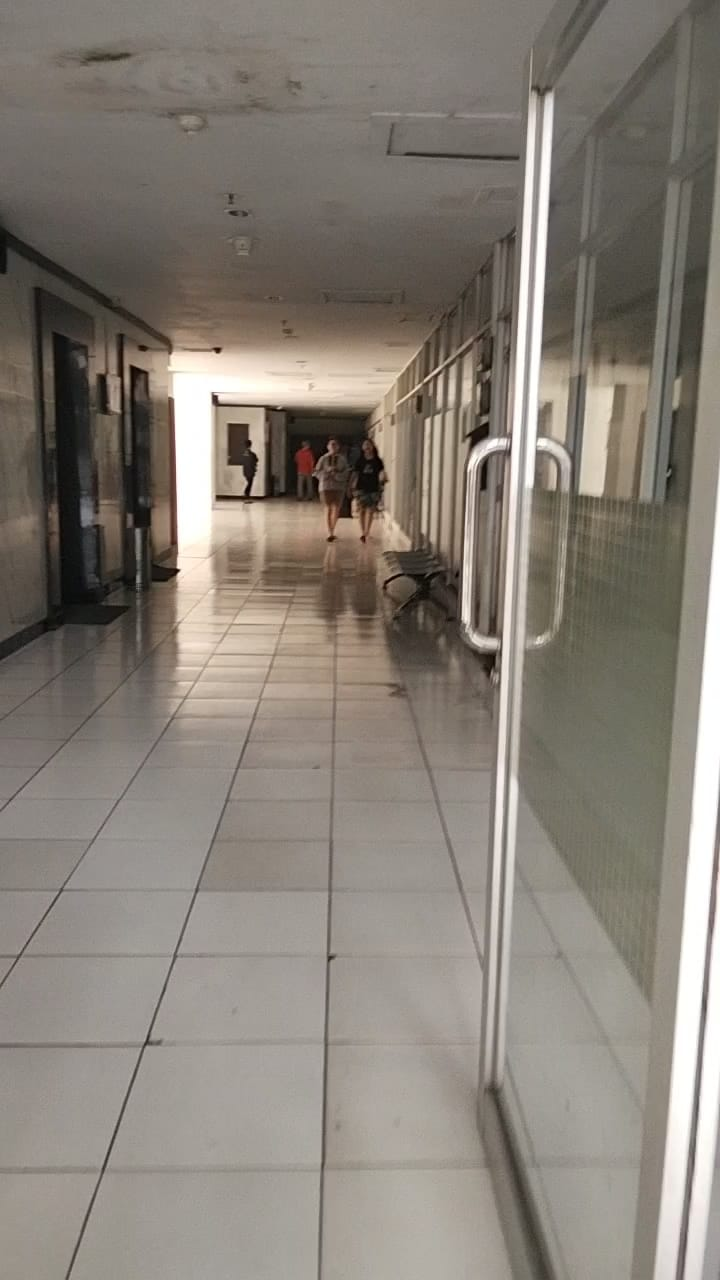
\includegraphics[width=\linewidth, max height=0.45\textheight]{Gambar/tampak depan ruangan2 agen.jpg}
%                 \caption{Lorong Tempat Ruangan Para Agen}
%                 \label{fig:tampak depan ruangan2 agen}
%             \end{minipage}
%         \end{figure}
        

%         \begin{figure}[H]
%             \centering
%             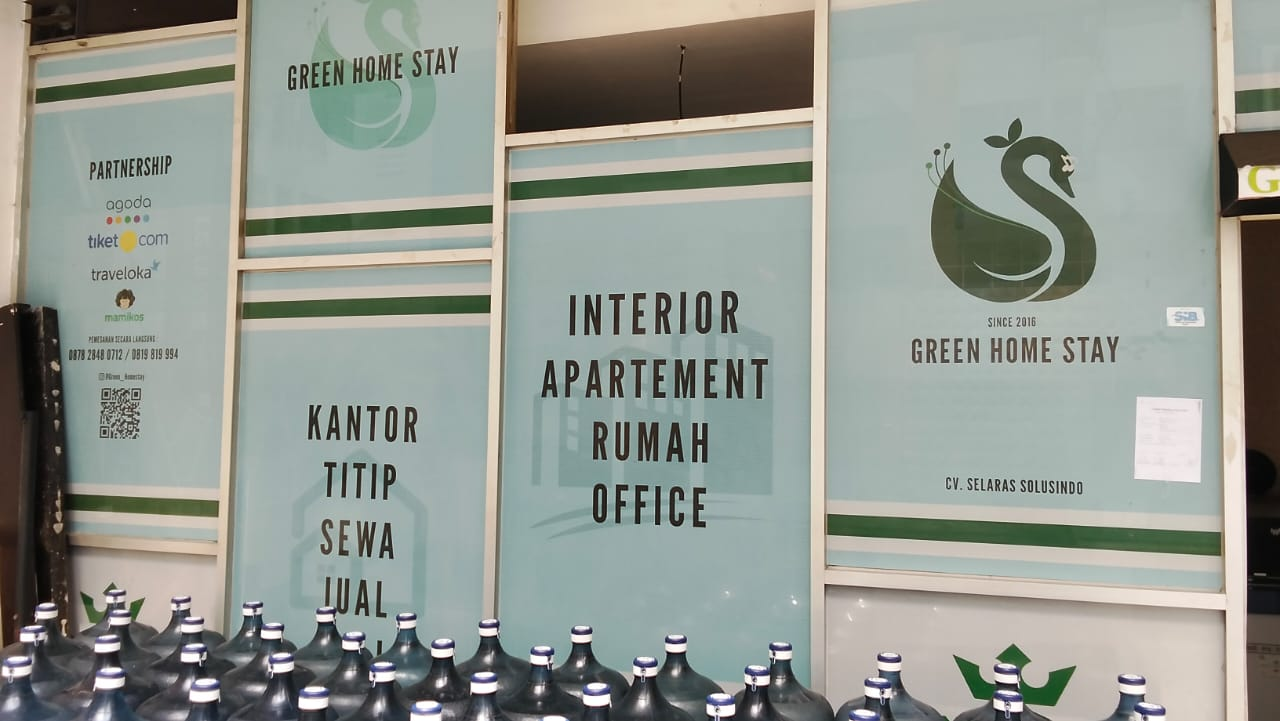
\includegraphics[width=0.6\textwidth, max height=0.5\textheight]{Gambar/ruang salah 1 agen.jpg}
%             \caption{Salah Satu Ruang Agen}
%             \label{fig:ruang salah 1 agen}
%         \end{figure}

        

%         Tempat parkir B1 diprioritaskan untuk para pemilik unit, pengurus, dan sepeda; sedangkan tempat parkir B2 diprioritaskan untuk para penyewa; dan tempat parkir B3 untuk sepeda motor.
%         \vspace{1cm}
%         \begin{figure}[H]
%             \centering
%             \begin{minipage}[b]{0.48\textwidth}
%                 \centering
%                 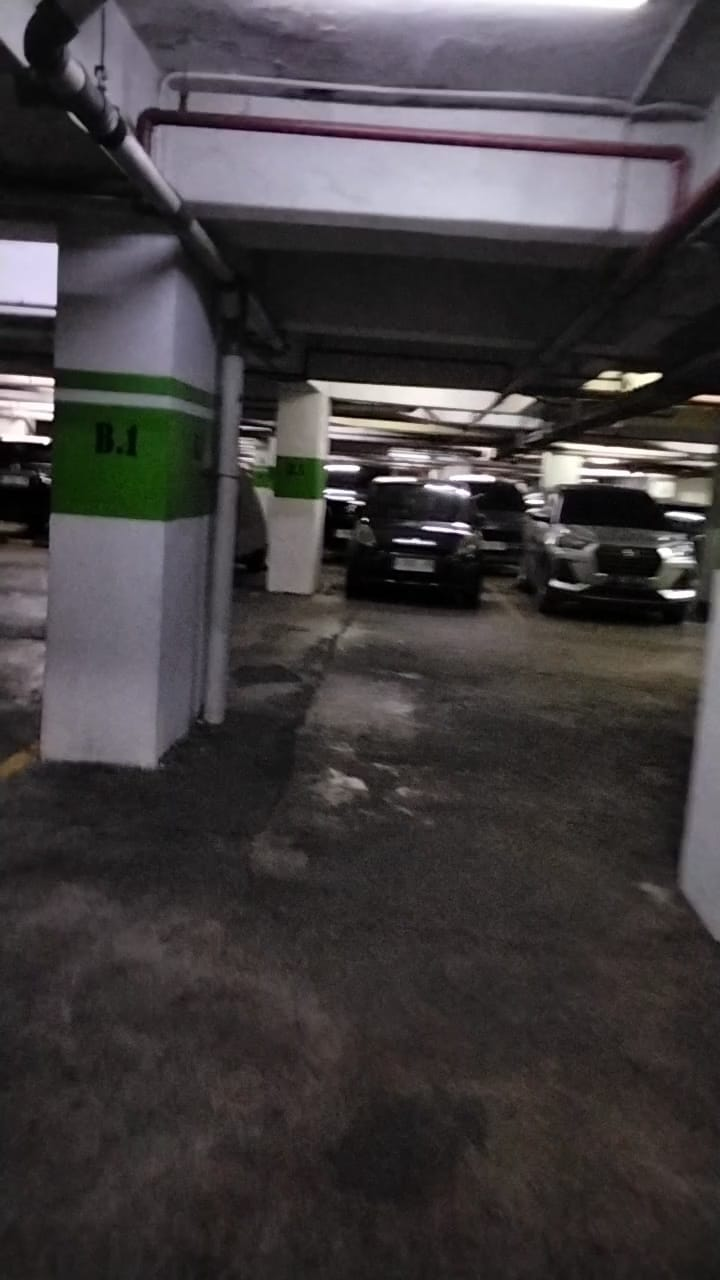
\includegraphics[width=\textwidth, height=0.45\textheight, keepaspectratio]{Gambar/parkir b1.jpg}
%                 \caption{Tempat Parkir B1}
%                 \label{fig:b1}
%             \end{minipage}
%             \hfill
%             \begin{minipage}[b]{0.48\textwidth}
%                 \centering
%                 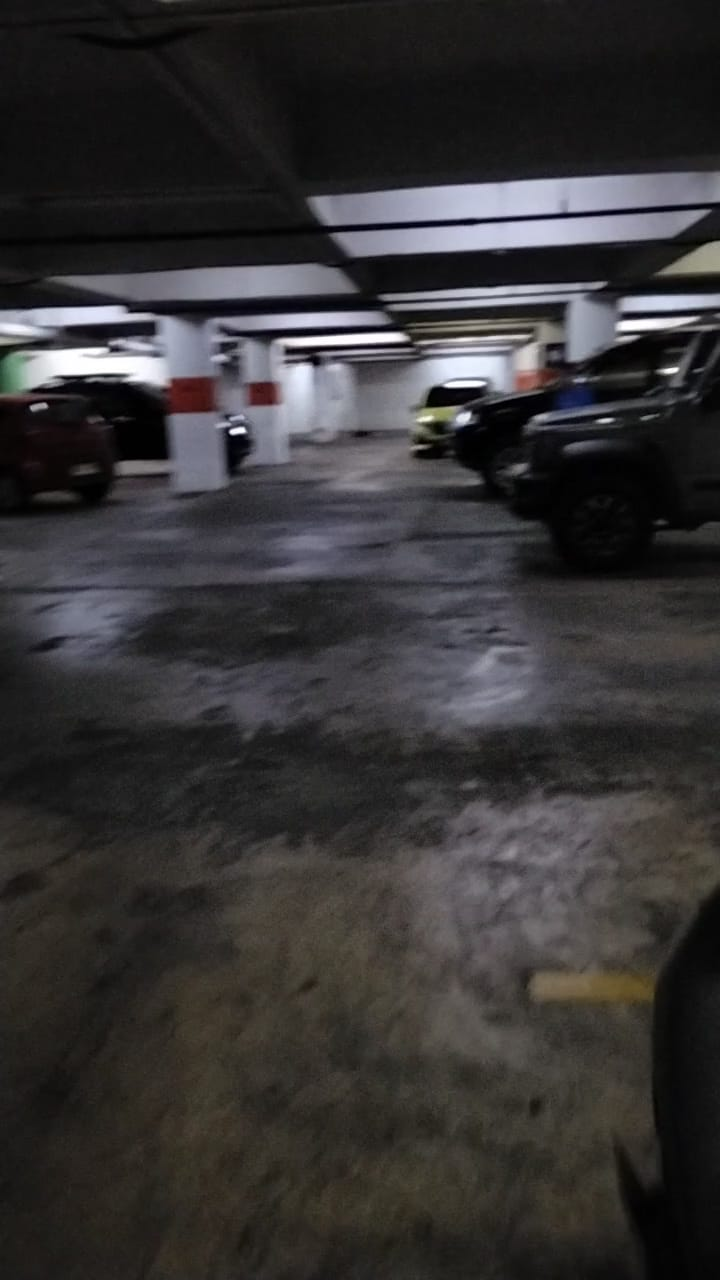
\includegraphics[width=\textwidth, height=0.45\textheight, keepaspectratio]{Gambar/parkir b2.jpg}
%                 \caption{Tempat Parkir B2}
%                 \label{fig:b2}
%             \end{minipage}
%         \end{figure}
        

%         \newpage
%         Ruang Badan Pengelola P3SRS berfungsi untuk mengajukan pengaduan, melakukan pembayaran parkir bulanan, dan membayar tagihan IPL.
%         \begin{figure}[H]
%             \centering
%             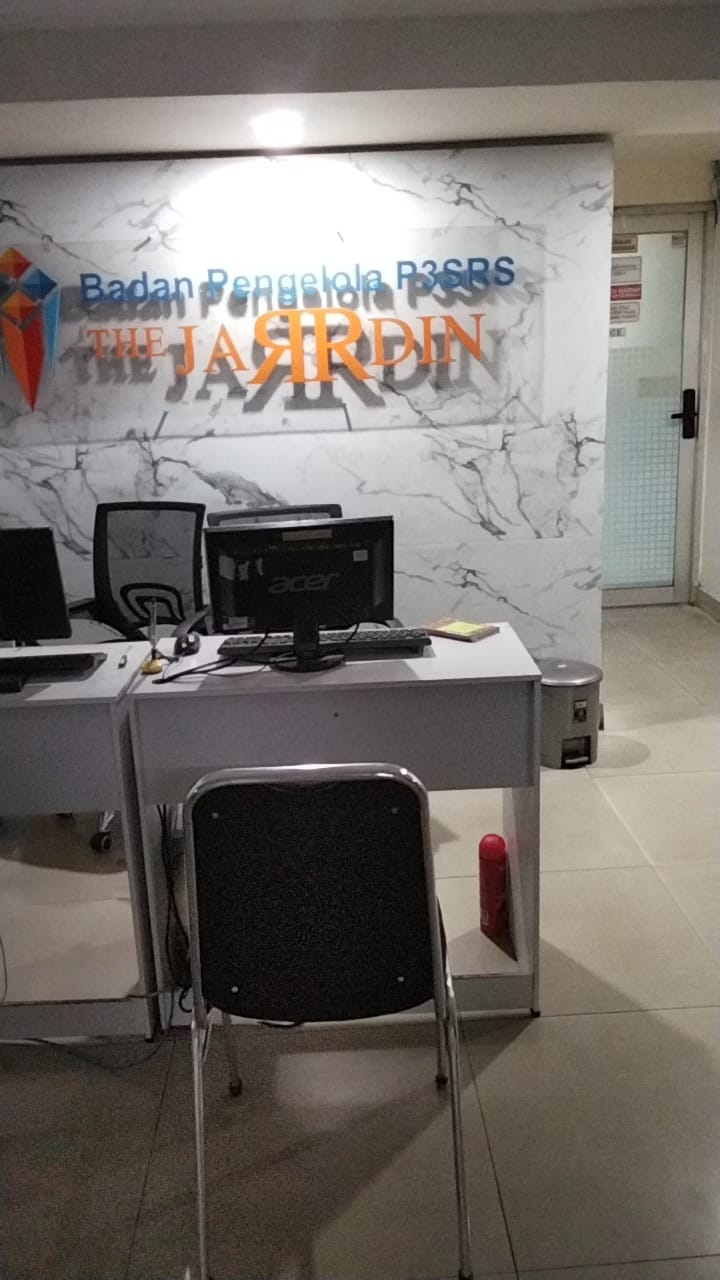
\includegraphics[width=0.5\textwidth, max height=0.45\textheight]{Gambar/ruang badan pengelola p3srs.jpg}
%             \caption{Tempat Parkir B2}
%             \label{fig:b2}
%         \end{figure}


%         \vspace{-2cm}
%         Berikut adalah ruangan-ruangan untuk keamanan dan pemeliharaan lingkungan Rusunami The Jarrdin.
%         \begin{figure}[H]
%             \centering
%             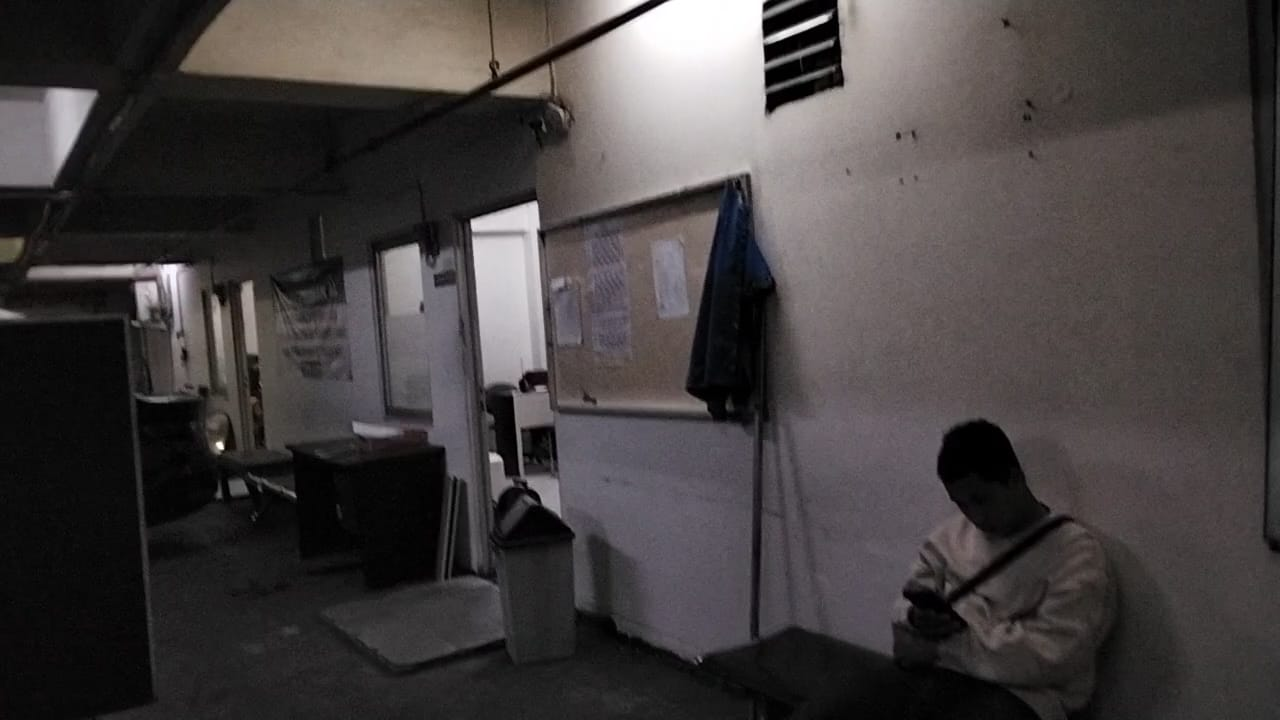
\includegraphics[width=0.65\textwidth, max height=0.55\textheight]{Gambar/ruangan-ruangan untuk para pemelihara.jpg}
%             \caption{Tampak Depan Ruangan-Ruangan untuk para Pemelihara}
%             \label{fig:ruang pemelihara}
%         \end{figure}

%         \begin{figure}[H]
%             \centering
%             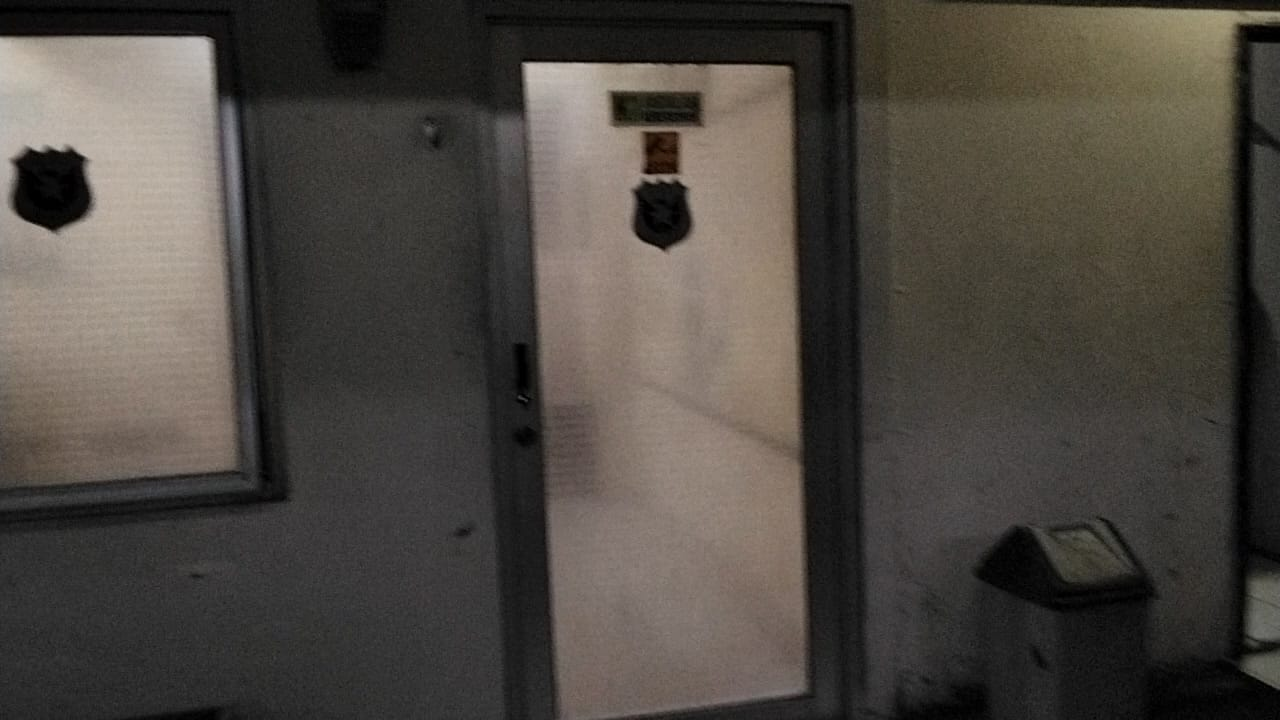
\includegraphics[width=0.5\textwidth, max height=0.45\textheight]{Gambar/ruang security.jpg}
%             \caption{Ruangan Keamanan}
%             \label{fig:ruang security}
%         \end{figure}

%         \begin{figure}[H]
%             \centering
%             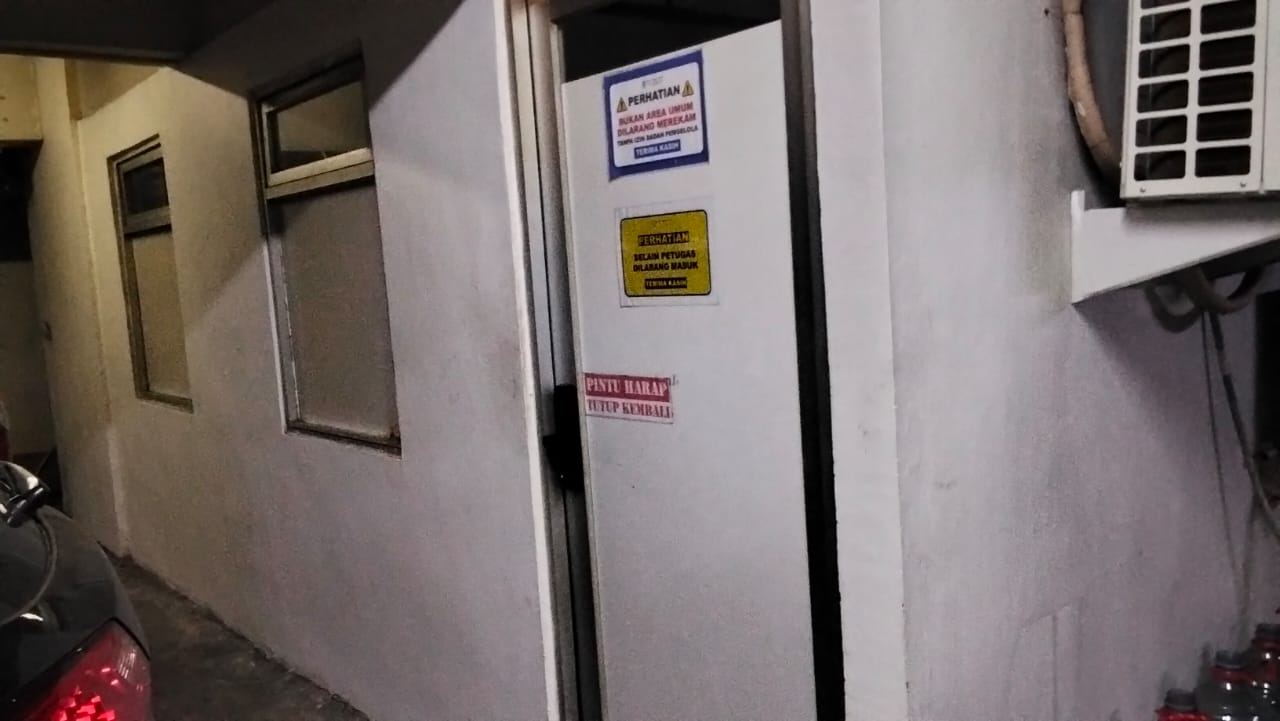
\includegraphics[width=0.5\textwidth, max height=0.45\textheight]{Gambar/ruang cctv.jpg}
%             \caption{Ruangan CCTV}
%             \label{fig:ruang cctv}
%         \end{figure}

%         \begin{figure}[H]
%             \centering
%             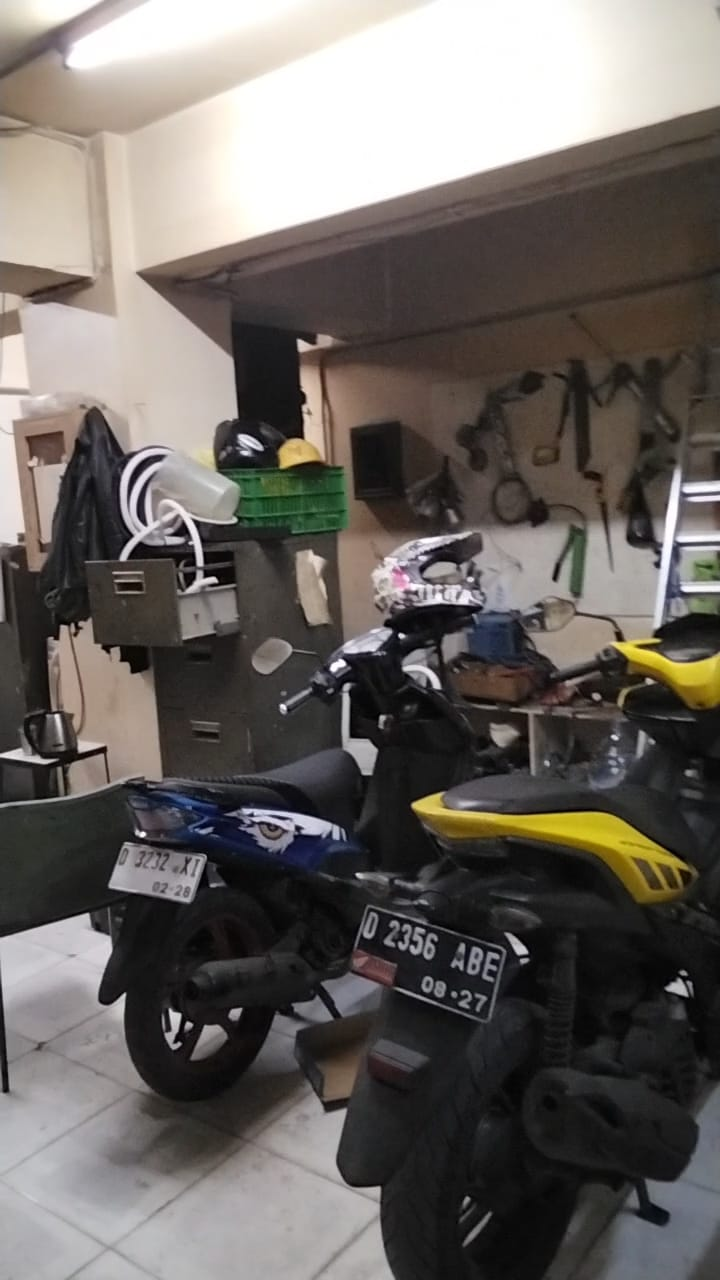
\includegraphics[width=0.5\textwidth, max height=0.45\textheight]{Gambar/ruang engineering.jpg}
%             \caption{Ruangan {\it Engineering}}
%             \label{fig:ruang engineering}
%         \end{figure}

%         Berikut contoh fasilitas yang disediakan oleh Rusunami The Jarrdin.
%         \begin{figure}[H]
%             \centering
%             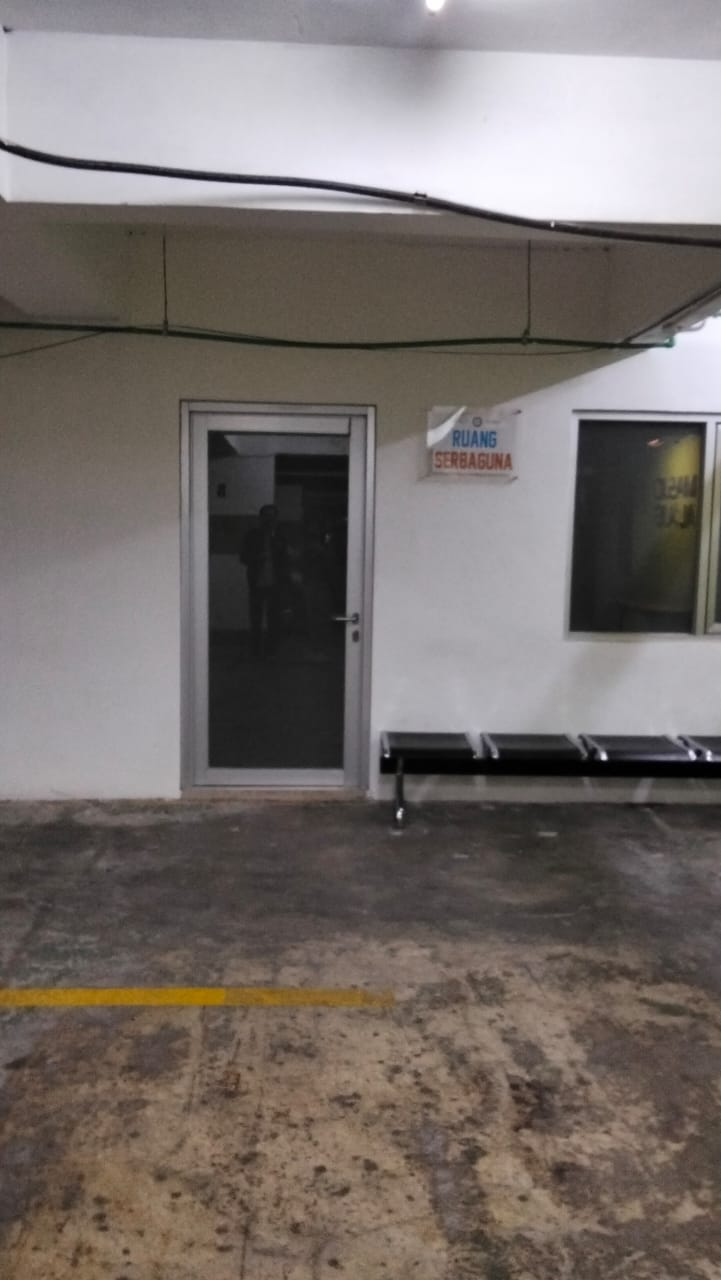
\includegraphics[width=0.5\textwidth, max height=0.4\textheight]{Gambar/fasilitas ruang serbaguna.jpg}
%             \caption{Fasilitas Ruang Serbaguna}
%             \label{fig:fasilitas ruang serbaguna}
%         \end{figure}

%         \begin{figure}[H]
%             \centering
%             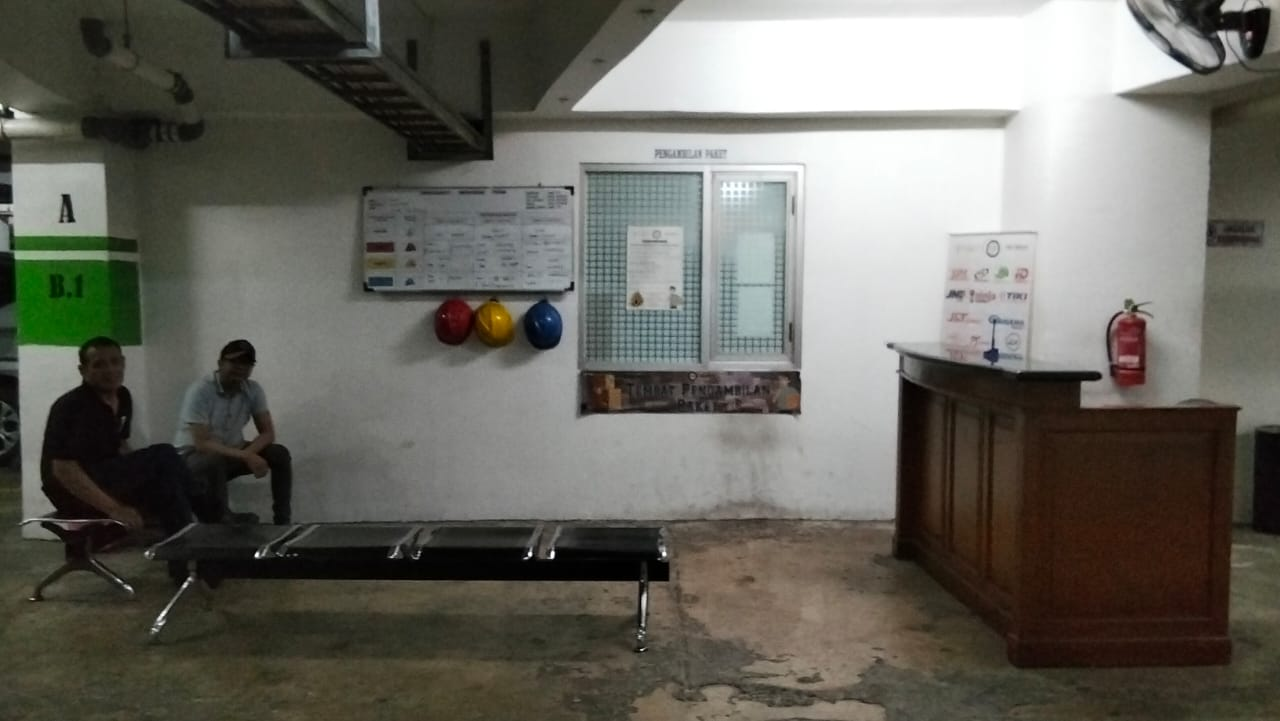
\includegraphics[width=0.5\textwidth, max height=0.45\textheight]{Gambar/tempat ambil paket.jpg}
%             \caption{Fasilitas Tempat Ambil Paket}
%             \label{fig:tempat ambil paket}
%         \end{figure}

%         \begin{figure}[H]
%             \centering
%             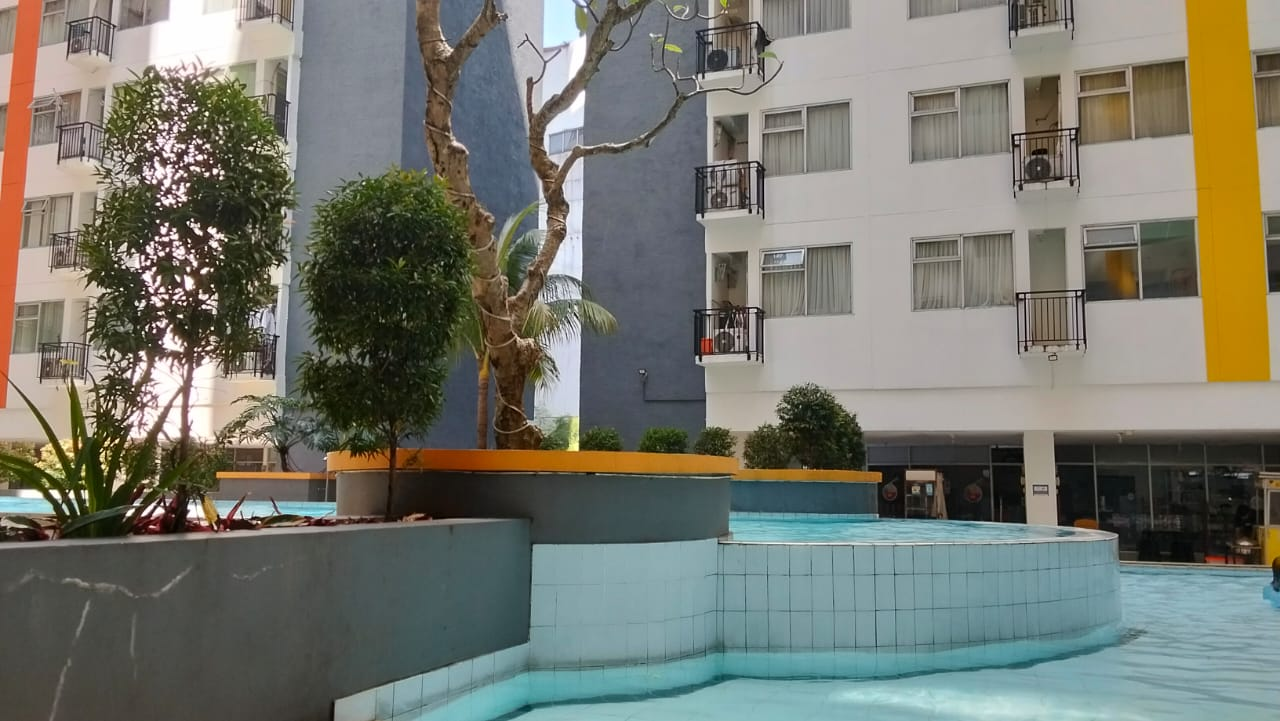
\includegraphics[width=0.5\textwidth, max height=0.45\textheight]{Gambar/kolam renang.jpg}
%             \caption{Fasilitas Kolam Renang}
%             \label{fig:fasilitas kolam renang}
%         \end{figure}

%         \begin{figure}[H]
%             \centering
%             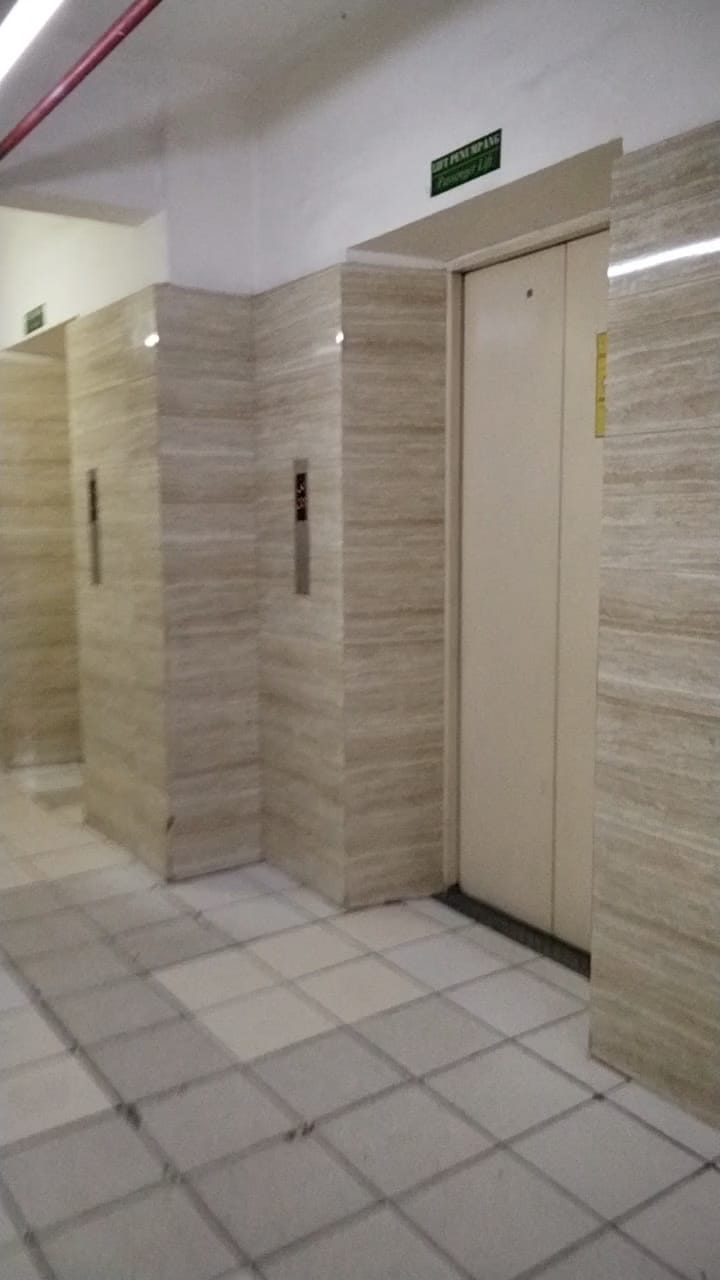
\includegraphics[width=0.6\textwidth, max height=0.4\textheight]{Gambar/lift.jpg}
%             \caption{Fasilitas Lift}
%             \label{fig:lift}
%         \end{figure}

        

%         % \vspace{-5cm}
%         Tersedianya berbagai akses keluar masuk ke kawasan The Jarrdin, seperti akses jalan untuk para pejalan kaki, tangga darurat, dan basement membuat keamanan tidak optimal.

%         % \vspace{-2cm}
%         \begin{figure}[H]
%             \centering
%             \begin{minipage}[b]{0.49\textwidth}
%                 \centering
%                 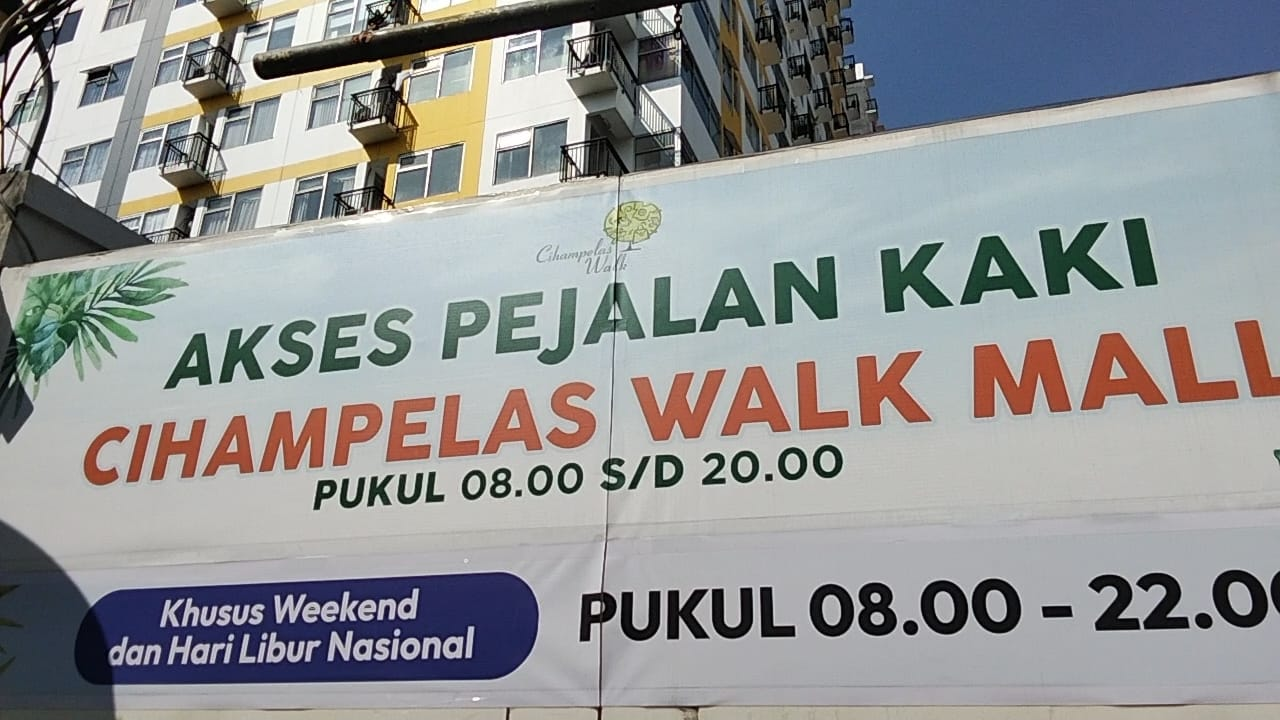
\includegraphics[width=\textwidth,height=0.5\textheight,keepaspectratio]{Gambar/fasilitas akses ke ciwalk.jpg}
%                 \caption{Fasilitas Akses Jalan Menuju Ciwalk}
%                 \label{fig:fasilitas-akses-ciwalk}
%             \end{minipage}
%             \hfill
%             \begin{minipage}[b]{0.49\textwidth}
%                 \centering
%                 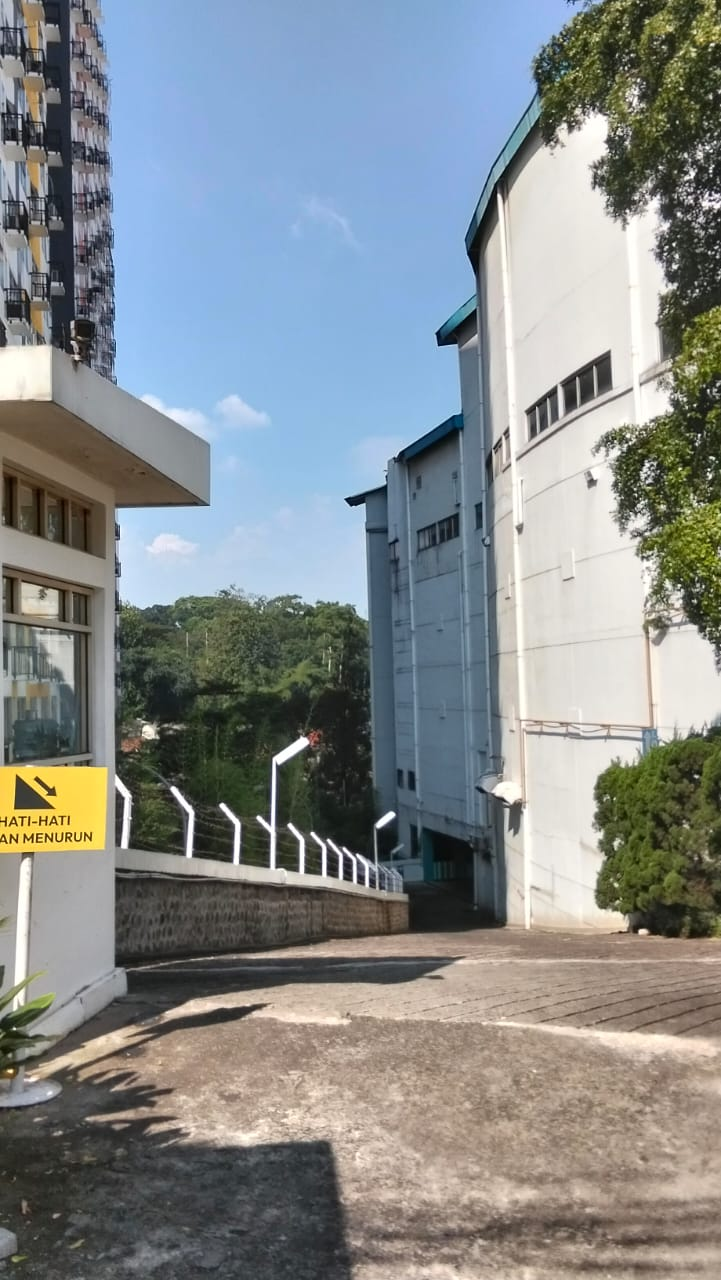
\includegraphics[width=0.6\textwidth,height=0.4\textheight,keepaspectratio]{Gambar/akses jalan menuju ciwalk.jpg}
%                 \caption{Akses Jalan Menuju Ciwalk}
%                 \label{fig:akses-jalan-ciwalk}
%             \end{minipage}
%         \end{figure}
        
%         \newpage
%         \begin{figure}[H]
%             \centering
%             % --- Gambar Kiri ---
%             \begin{minipage}[t]{0.48\textwidth}
%                 \centering
%                 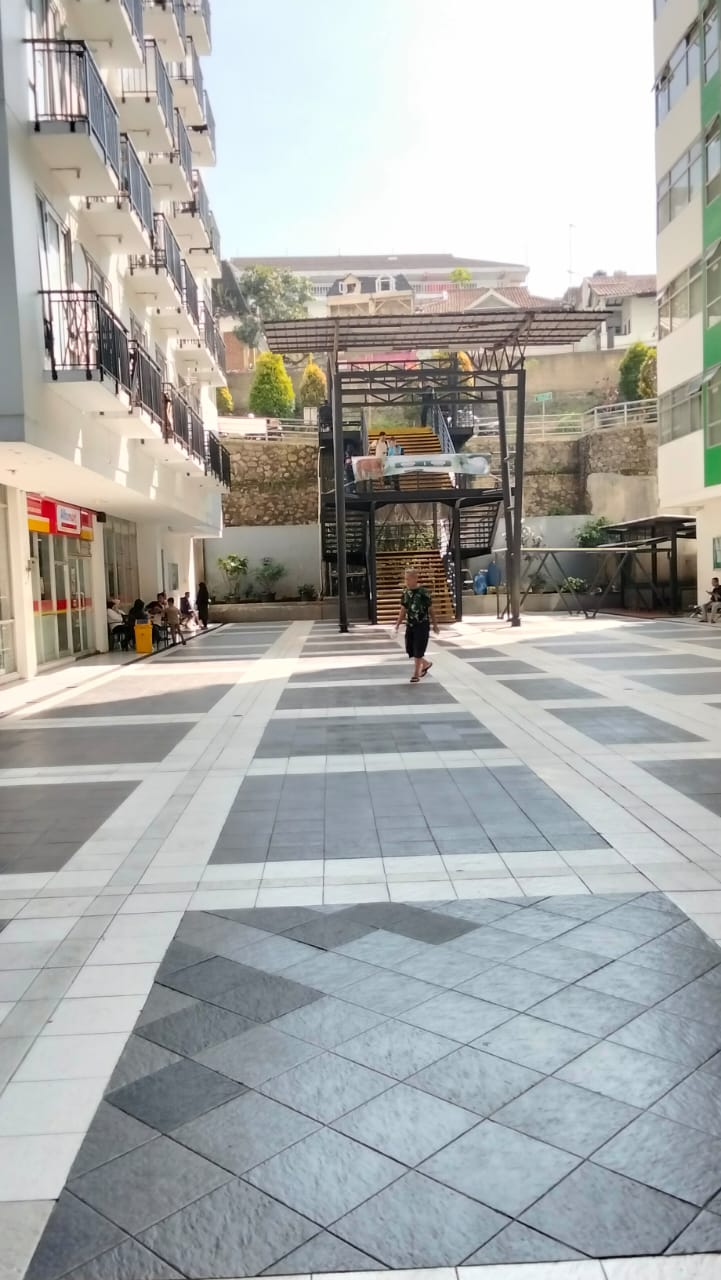
\includegraphics[width=\linewidth, max height=0.45\textheight]{Gambar/akses tangga untuk pejalan kaki.jpg}
%                 \caption{Fasilitas Akses Tangga untuk Pejalan Kaki}
%                 \label{fig:akses tangga untuk pejalan kaki}
%             \end{minipage}
%             \hfill
%             % --- Gambar Kanan ---
%             \begin{minipage}[t]{0.48\textwidth}
%                 \centering
%                 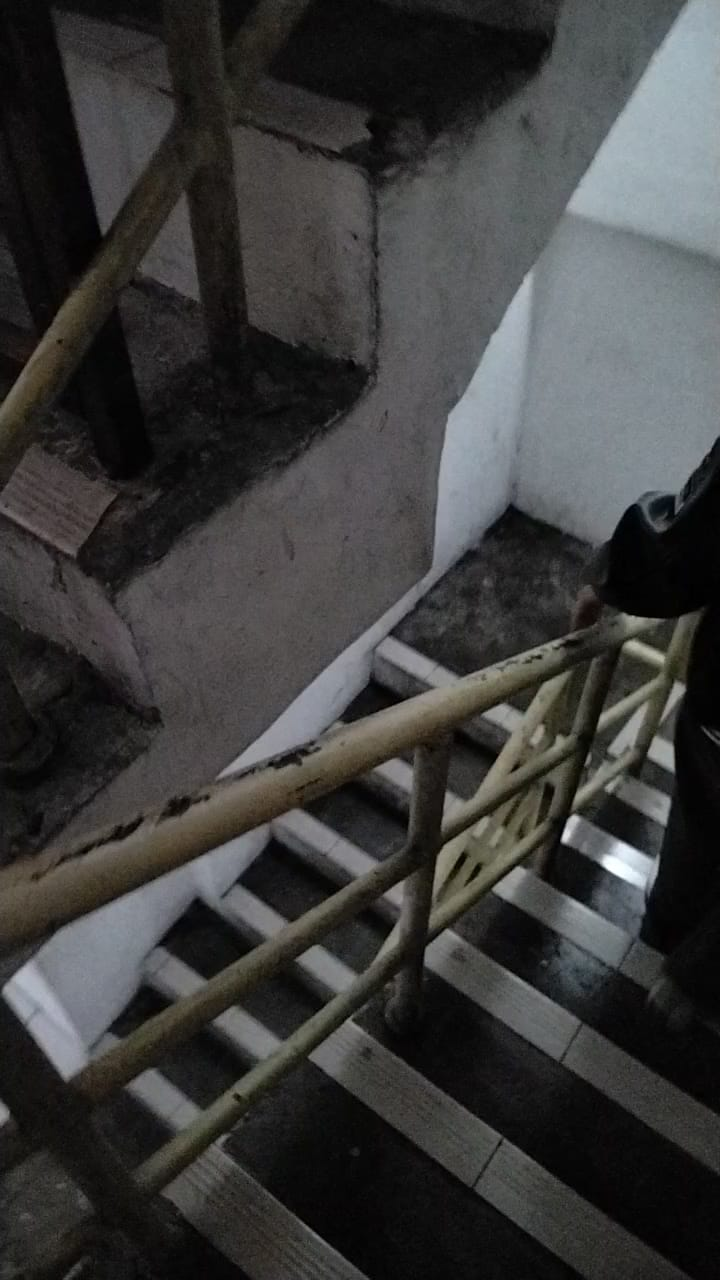
\includegraphics[width=\linewidth, max height=0.45\textheight]{Gambar/tangga darurat.jpg}
%                 \caption{Fasilitas Tangga Darurat}
%                 \label{fig:tangga darurat}
%             \end{minipage}
%         \end{figure}
        

% % \newpage
% \subsection{Kebutuhan Fungsional Sistem}
% Berdasarkan hasil analisis masalah dan masukan dari narasumber, sistem yang akan dibangun harus memenuhi kebutuhan fungsional sebagai berikut.

% \begin{enumerate}
%     \item \textbf{Manajemen data terpusat dengan kontrol akses berjenjang}\\
%     Sistem harus memfasilitasi input data oleh agen, namun membatasi akses data sesuai peran. Agen hanya dapat melihat data kelolaannya sendiri, sementara Ketua Agen, P3SRS, dan PKJ memiliki akses global untuk pengawasan dan deteksi duplikasi penyewa antar-agen.
    
%     \item \textbf{Master data unit}\\
%     Untuk meminimalisir kesalahan input manual dan mempercepat proses, sistem perlu menyediakan {master data} unit. Agen cukup memilih unit dari daftar yang tersedia yang telah dipetakan sesuai hak kelola mereka.
    
%     \item \textbf{Pencatatan riwayat dan log aktivitas}\\
%     Setiap perubahan data (seperti perpanjangan sewa, pengeditan metode bayar, atau perubahan status check-out) harus tercatat dalam \textit{log history} yang tidak dapat dihapus. Fitur ini krusial untuk audit jejak digital apabila terjadi sengketa atau investigasi pelanggaran.
    
%     \item \textbf{Pelaporan pelanggaran visual}\\
%     Sistem harus mendukung unggahan bukti foto pelanggaran yang ditampilkan pada \textit{dashboard} sebagai rekam jejak digital. Selain untuk mendokumentasikan pelanggaran fisik (seperti kerusakan unit, temuan barang terlarang, atau kondisi unit yang tidak layak), penayangan bukti visual ini juga bertujuan memberikan efek jera bagi para pelanggar.
    
%     \item \textbf{Deteksi profil risiko penyewa}\\
%     Sistem perlu memiliki fitur untuk mendeteksi nama atau NIK penyewa yang muncul berulang kali di berbagai agen berbeda (\textit{hopping}), yang bisa menjadi indikator perilaku mencurigakan.
% \end{enumerate}


\section{Analisis Masalah dan Kebutuhan Sistem}
\label{sec:analisis}

Analisis masalah dilakukan melalui pendekatan kualitatif dengan melakukan wawancara mendalam serta survei lapangan terhadap pemangku kepentingan utama di lingkungan Rusunami The Jarrdin Cihampelas (RTJC).

\subsection{Kondisi Faktual Pengelolaan Penyewaan}

\begin{figure}[h]
    \centering
    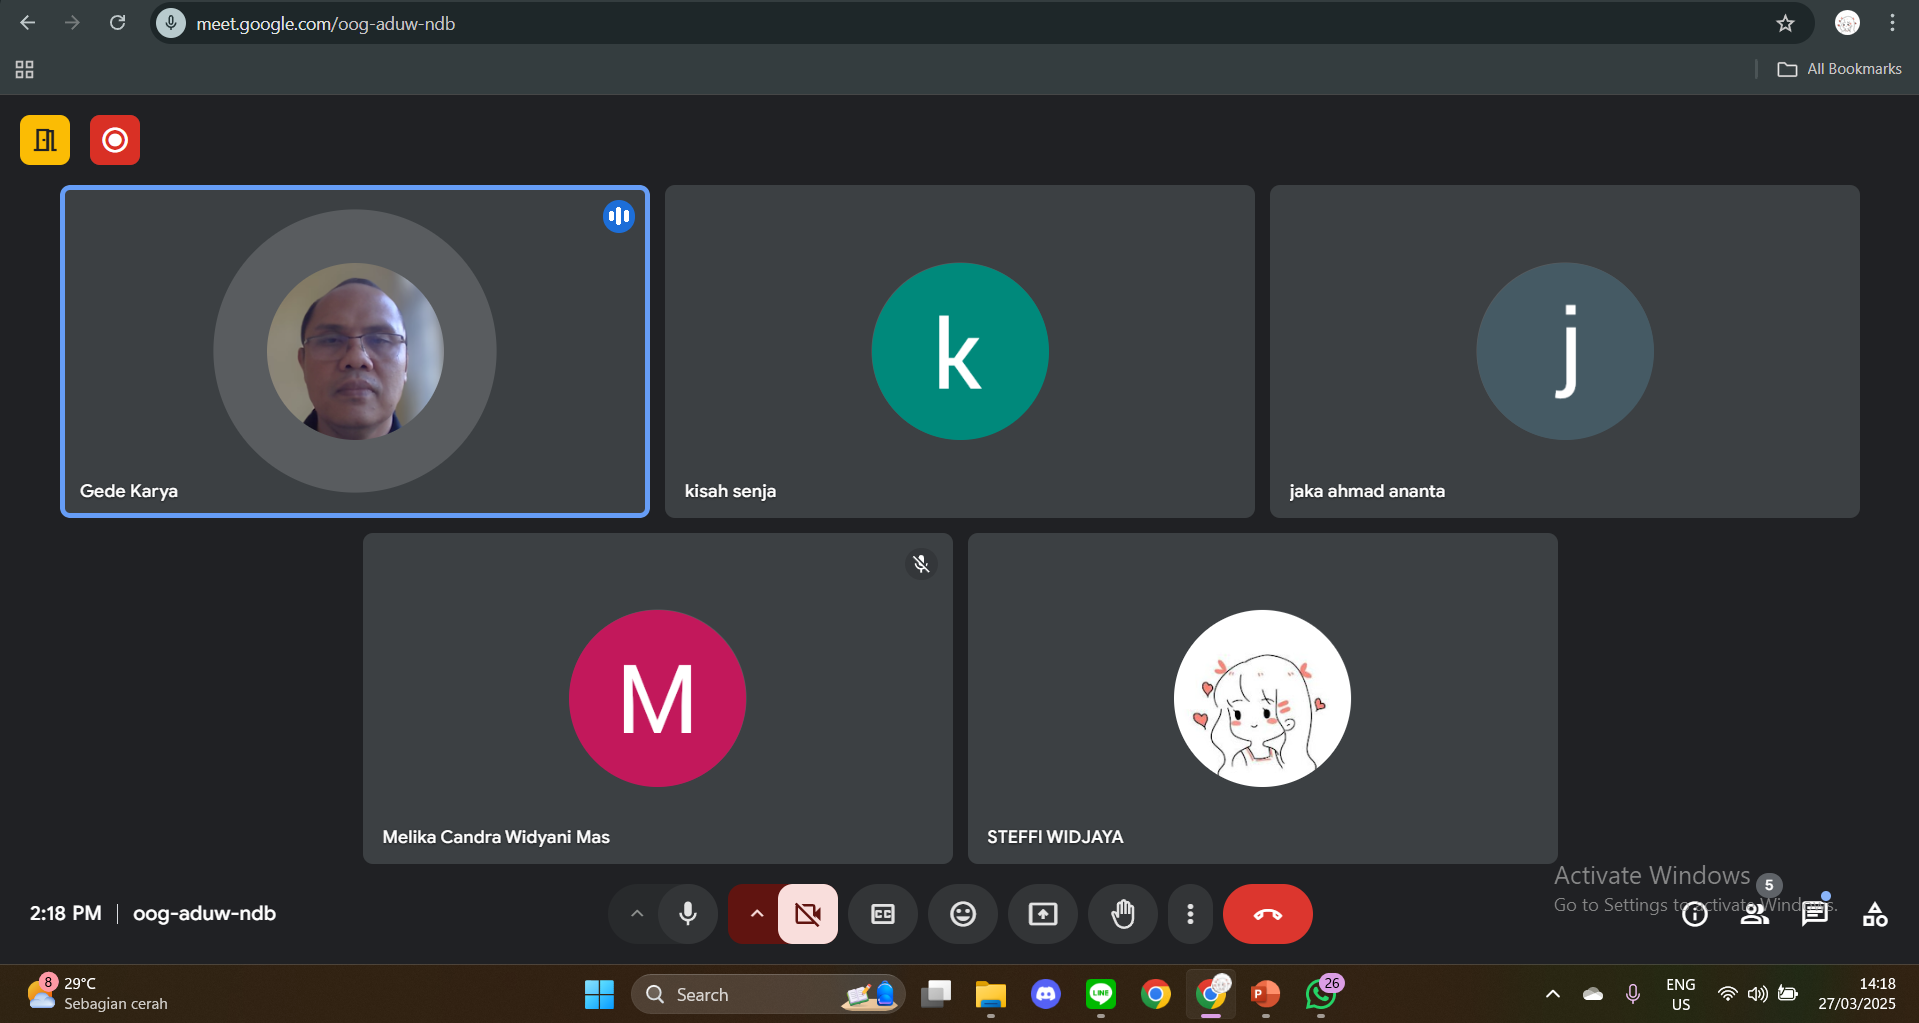
\includegraphics[width=0.45\textwidth]{Gambar/dokumentasi wawancara.png}
    \caption{Dokumentasi Pertemuan Wawancara dengan Narasumber secara {\it Online}}
    \label{fig:wawancara_online}
\end{figure}

% Berdasarkan rangkaian kegiatan pengumpulan data yang telah dilakukan—meliputi wawancara awal pada tanggal 23 Maret 2025 (secara daring melalui Google Meet), wawancara dan survei lapangan untuk pemetaan kebutuhan pada tanggal 31 Mei 2025 (di lokasi Apartemen The Jarrdin), serta sesi konfirmasi purwarupa sistem dan penjaringan masukan pada tanggal 13 Oktober 2025 (di lokasi Apartemen The Jarrdin)—bersama dengan pihak pengelola (Ketua Agen, P3SRS, atau PKJ) yang terdiri dari perwakilan pelaku komersil Paguyuban Komersil Jarrdin (PKJ) serta pengurus Perhimpunan Pemilik dan Penghuni Satuan Rumah Susun (P3SRS) (Bapak Rey, Bapak Jaka, dan Bapak Diki), teridentifikasi beberapa kondisi faktual dan poin krusial terkait tata kelola saat ini sebagai berikut.

Berdasarkan rangkaian kegiatan pengumpulan data yang telah dilakukan (sejalan dengan karakteristik pengelolaan dan dinamika penghuni sebagaimana dijelaskan pada kajian teori terkait rumah susun di Subbab~\ref{sec:rumah_susun})—meliputi wawancara awal pada tanggal 23 Maret 2025 (secara daring melalui Google Meet), wawancara dan survei lapangan untuk pemetaan kebutuhan pada tanggal 31 Mei 2025 (di lokasi Apartemen The Jarrdin), serta sesi konfirmasi purwarupa sistem dan penjaringan masukan pada tanggal 13 Oktober 2025 (di lokasi Apartemen The Jarrdin)—bersama dengan pihak pengelola yang terdiri dari perwakilan agen Paguyuban Komersil Jarrdin (PKJ) serta pengurus Perhimpunan Pemilik dan Penghuni Satuan Rumah Susun (P3SRS) (Bapak Rey, Bapak Jaka, dan Bapak Diki), teridentifikasi beberapa kondisi faktual dan poin krusial terkait tata kelola saat ini sebagai berikut.

\begin{enumerate}
    \item \textbf{Desentralisasi data dan pengelolaan manual} \\
    Saat ini, sistem penyewaan unit dikelola secara terpisah dan manual tanpa bantuan sistem teknologi terintegrasi. Tidak ada basis data terpusat yang memungkinkan pihak pengelola (Ketua Agen, P3SRS, atau PKJ) untuk memantau aktivitas penyewaan secara menyeluruh. 
    \begin{itemize}
        \item Data penyewaan belum tersimpan dalam sistem digital yang terstruktur, melainkan dikelola masing-masing oleh pihak agen atau pelaku komersil.
        \item Ketidakhadiran data historis yang terdokumentasi dengan baik menyulitkan deteksi dini terhadap penyewa yang berpindah-pindah antar-pelaku komersil untuk menghindari pelacakan rekam jejak buruk.
    \end{itemize}

    \item \textbf{Keterbatasan akses informasi dan hierarki} \\
    Pelaku komersil hanya memiliki visibilitas terhadap data unit yang mereka kelola sendiri. Kebutuhan di lapangan menunjukkan perlunya hierarki akses di mana peran otoritas pengelola (Ketua Agen, P3SRS, atau PKJ) dapat melihat rekapitulasi data dari seluruh pelaku komersil untuk keperluan pengawasan dan evaluasi. Saat ini, belum ada sistem \textit{data capture} yang memungkinkan penarikan data dari pelaku komersil atau penyewa untuk kebutuhan ini.

    \item \textbf{Standarisasi pencatatan dan administrasi} \\
    Input data masih bervariasi antar-pelaku komersil. Meskipun penyewa dan pemilik unit diwajibkan menandatangani surat perjanjian sewa untuk menghindari risiko kriminal dan kelalaian, data transaksi tersebut belum dimanfaatkan untuk analisis. Diperlukan standarisasi input digital yang mencakup hal berikut.
    \begin{itemize}
        \item Identitas penyewa (NIK) dan email agen (pelaku komersil) penanggung jawab.
        \item Unit kamar yang disewa.
        \item Status kewarganegaraan penyewa.
        \item Status pernikahan (pasutri/bukan) dan metode pembayaran.
        \item Waktu \textit{check-in/check-out} serta durasi menginap (harian/mingguan/bulanan).
    \end{itemize}
    Data-data ini divalidasi oleh narasumber sebagai variabel yang sangat memungkinkan untuk dikumpulkan dan krusial untuk keperluan analisis perilaku.

    \item \textbf{Pengawasan manual dan pola deteksi reaktif} \\
    Saat ini belum ada sistem peringatan dini (\textit{early warning}) berbasis pola data administratif. Fakta lapangan menunjukkan (hal ini beririsan erat dengan teori mengenai indikator perilaku berisiko pada Subbab~\ref{sec:pola_perilaku}):
    \begin{itemize}
        \item pelanggaran sering kali baru diketahui setelah penyewa menginap lebih dari dua hari, saat layanan kebersihan (\textit{cleaning service}) menemukan barang mencurigakan di tempat sampah (seperti alat kontrasepsi atau jarum suntik dalam jumlah tidak wajar),
        \item kasus yang paling sering terjadi adalah praktik prostitusi dan penyalahgunaan narkoba,
        \item tidak ada pola visual (gaya berpakaian/penampilan) yang dapat dijadikan acuan. Pelanggaran dapat dilakukan oleh individu maupun kelompok, serta terjadi pada penyewa harian (transit/liburan) maupun bulanan.
        \item saat penyewa bermasalah ditemukan, belum ada dokumentasi formal mengenai proses penyelesaian masalah tersebut, sehingga pola pelanggaran sulit dipelajari secara historis.
    \end{itemize}
\end{enumerate}

        \begin{figure}[H]
            \centering
            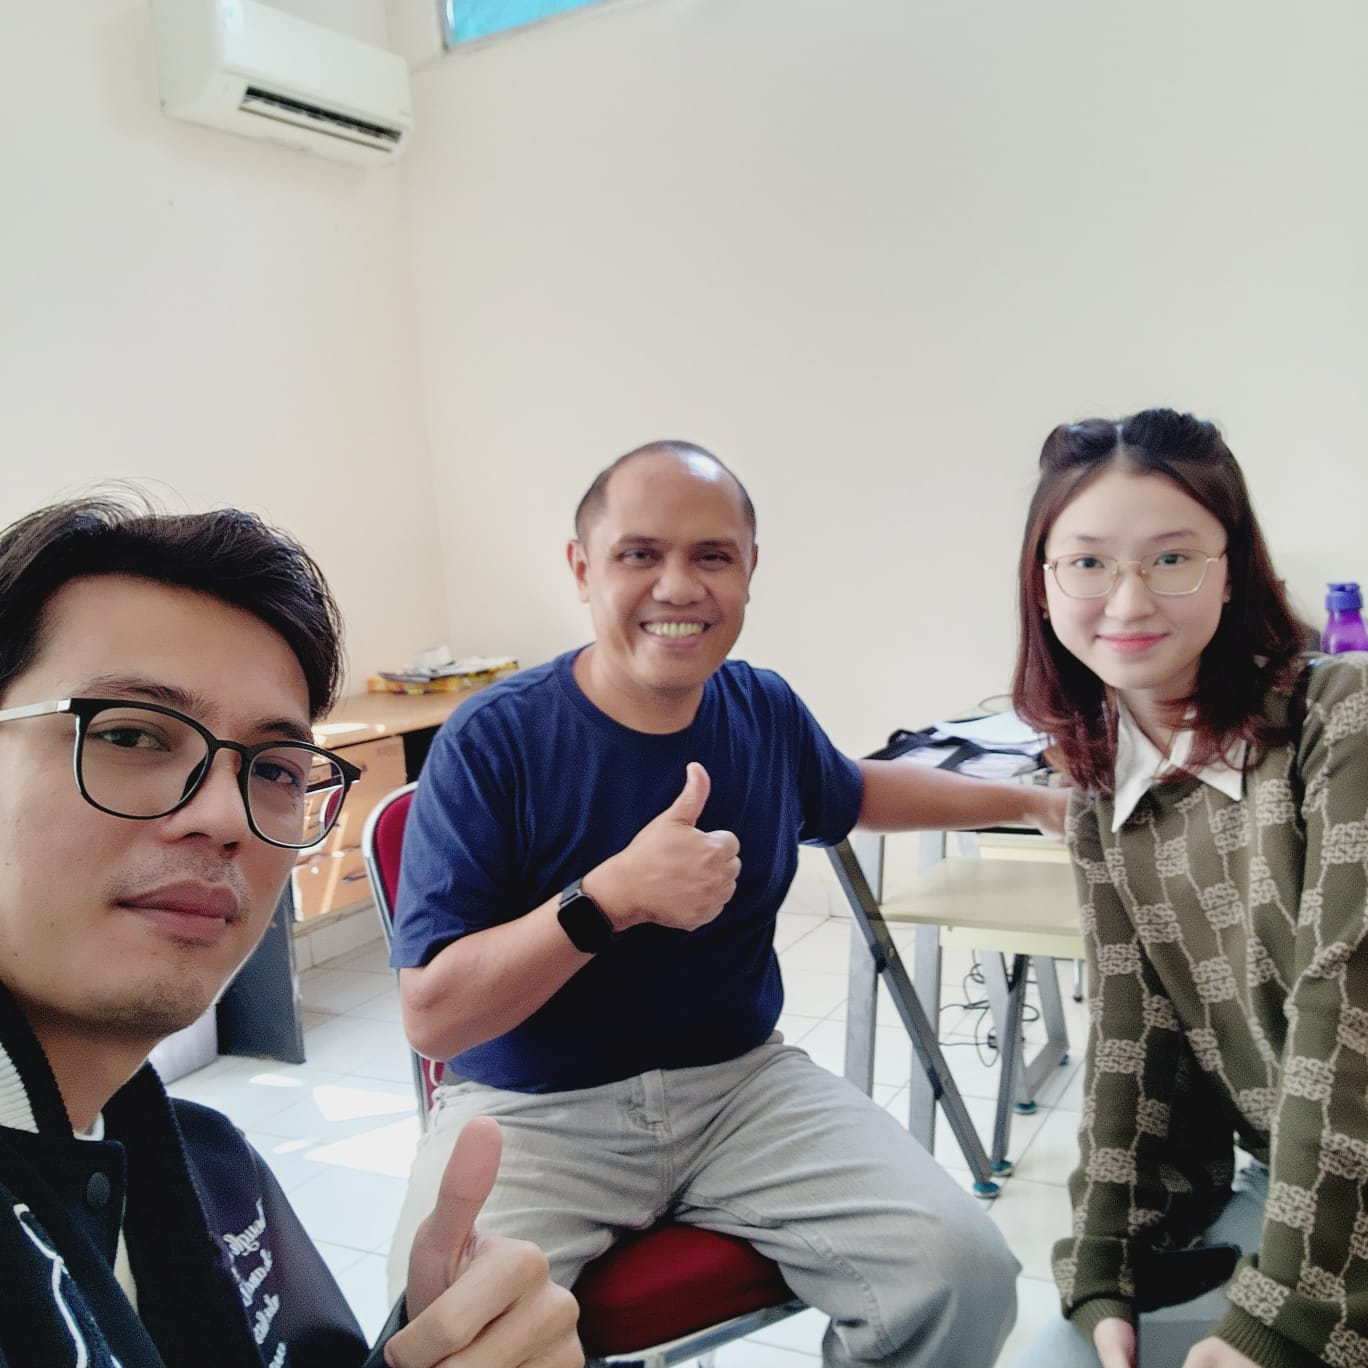
\includegraphics[width=0.45\textwidth, max height=0.25\textheight]{Gambar/dokumentasi wawancara2.jpg}
            \caption{Dokumentasi Pertemuan Wawancara dengan Narasumber secara {\it Offline} pada tanggal 31 Mei 2025}
            \label{fig:dokumentasi wawancara2}
        \end{figure}

        \begin{figure}[H]
            \centering
            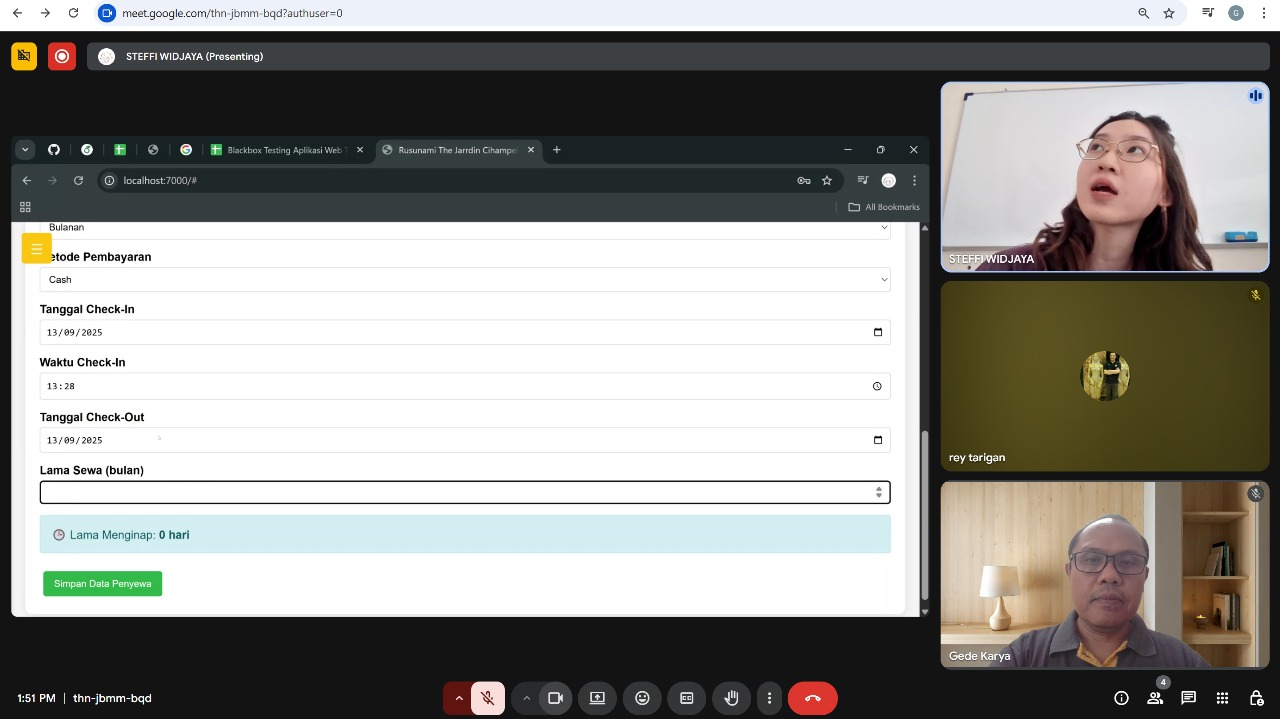
\includegraphics[width=0.45\textwidth, max height=0.25\textheight]{Gambar/dokumentasi wawancara3.jpeg}
            \caption{Dokumentasi Pertemuan Wawancara dengan Narasumber secara {\it Offline} pada tanggal 13 September 2025}
            \label{fig:dokumentasi wawancara3}
        \end{figure}

% \newpage
Selain wawancara daring, survei lapangan juga dilaksanakan guna mendata kondisi fisik dan fasilitas yang ada. Melalui kegiatan ini, diperoleh pula berbagai informasi mengenai sistem sewa, fasilitas, serta struktur pengelolaan di kawasan hunian tersebut. The Jarrdin memiliki total sekitar 2.400 unit yang terbagi ke dalam beberapa tipe, yakni tipe studio (18~m\textsuperscript{2} dan 24~m\textsuperscript{2}) serta tipe dua kamar (33~m\textsuperscript{2} dan 40~m\textsuperscript{2}). Unit tipe studio terdiri atas satu ruangan multifungsi yang menggabungkan area tidur, dapur, dan ruang tamu; sedangkan tipe dua kamar memiliki pemisahan ruang yang lebih tegas, mencakup kamar tidur terpisah, dapur, serta ruang tamu.

\vspace{0.5cm} Sistem penyewaan unit menerapkan skema ``titip sewa'' kepada agen (pelaku komersil). Dalam skema ini, pemilik unit menyerahkan pengelolaan kepada pelaku komersil dengan kesepakatan nilai kontrak bulanan yang tetap, terlepas dari apakah unit tersebut berhasil disewakan atau tidak. Bapak Diki Andrian Permana, salah satu perwakilan pelaku komersil yang diwawancarai, menjelaskan bahwa segala permasalahan yang dialami penyewa akan diarahkan terlebih dahulu kepada tim \textit{Tenant Relation} (TR) untuk penanganan awal. Syarat penitipan unit mengharuskan pemilik menyerahkan sejumlah dokumen, antara lain KTP pemilik dan pelaku komersil, PPJB (Perjanjian Pengikatan Jual Beli), serta surat perjanjian sewa-menyewa.

\vspace{0.5cm} Kawasan The Jarrdin terdiri atas empat tower dengan identitas warna yang berbeda, yakni Tower A (kuning), Tower B (hijau), Tower C (biru), dan Tower D (oranye). Fasilitas yang tersedia terbilang lengkap, meliputi kolam renang, akses langsung ke Cihampelas Walk (Ciwalk), area parkir basement, lift, ruang tunggu, supermarket, masjid, dan gereja GBI. Selain itu, terdapat area parkir darurat di lantai B2 yang difungsikan sebagai titik penanganan awal apabila terjadi pelanggaran atau situasi darurat. Terkait durasi sewa, unit dapat disewakan secara harian hingga mingguan. Pada sewa harian, biaya IPL (Iuran Pemeliharaan Lingkungan) dan token listrik ditanggung oleh penyewa, sedangkan untuk sewa bulanan, biaya tersebut menjadi tanggung jawab pemilik unit.

\vspace{0.5cm} Pengelolaan Rusunami dijalankan oleh pengurus di bawah pengawasan P3SRS (Perhimpunan Pemilik dan Penghuni Satuan Rumah Susun), yang anggotanya terdiri dari para pemilik unit sesuai ketentuan AD/ART. Struktur kepengurusan mencatat beberapa nama, antara lain Bapak Fendy Efendi (Ketua), Rudi Wiranata Kusumah (Sekretaris), serta Dewi Juwita dan Cici Pricillia Susanto (Bendahara). Bidang operasional diisi oleh Bapak Jaka (Kepenghunian) dan Bapak Rey (Pengelolaan), sementara fungsi pengawasan dijalankan oleh Bapak Agus Anwar, Bapak Erwin, dan Bapak Gede. Di sisi lain, aspek komersial dikelola oleh komunitas PKJ (Paguyuban Komersil Jarrdin) yang dipimpin oleh Bapak Hans, dibantu oleh Bapak Diki selaku sekretaris dan Ibu Marliana Furey sebagai bendahara.

\vspace{0.5cm} Tarif parkir di kawasan ini telah ditetapkan sebesar Rp25.000,00 per hari untuk mobil dan Rp15.000,00 untuk motor. Bagi penghuni yang berlangganan bulanan, biaya parkir motor dikenakan Rp75.000,00 dan mobil sebesar Rp150.000,00. Mengenai penanganan ketertiban, penghuni atau penyewa yang melakukan pelanggaran akan diarahkan ke area B2 untuk ditindaklanjuti oleh pengelola, dengan melibatkan orang tua, pelaku komersil bersangkutan, atau pihak kepolisian jika diperlukan. Berikut terlampir dokumentasi visual yang mencakup foto unit setiap tipe, tampilan depan ruang pelaku komersil, serta berbagai fasilitas yang tersedia di kawasan The Jarrdin.
        
        % \newpage
        % --- GRUP 1: TIPE STUDIO (2x2) ---
        \begin{figure}[htbp]
            \centering
            % Baris 1, Gambar 1 (Kiri)
            \begin{minipage}[t]{0.48\textwidth}
                \centering
                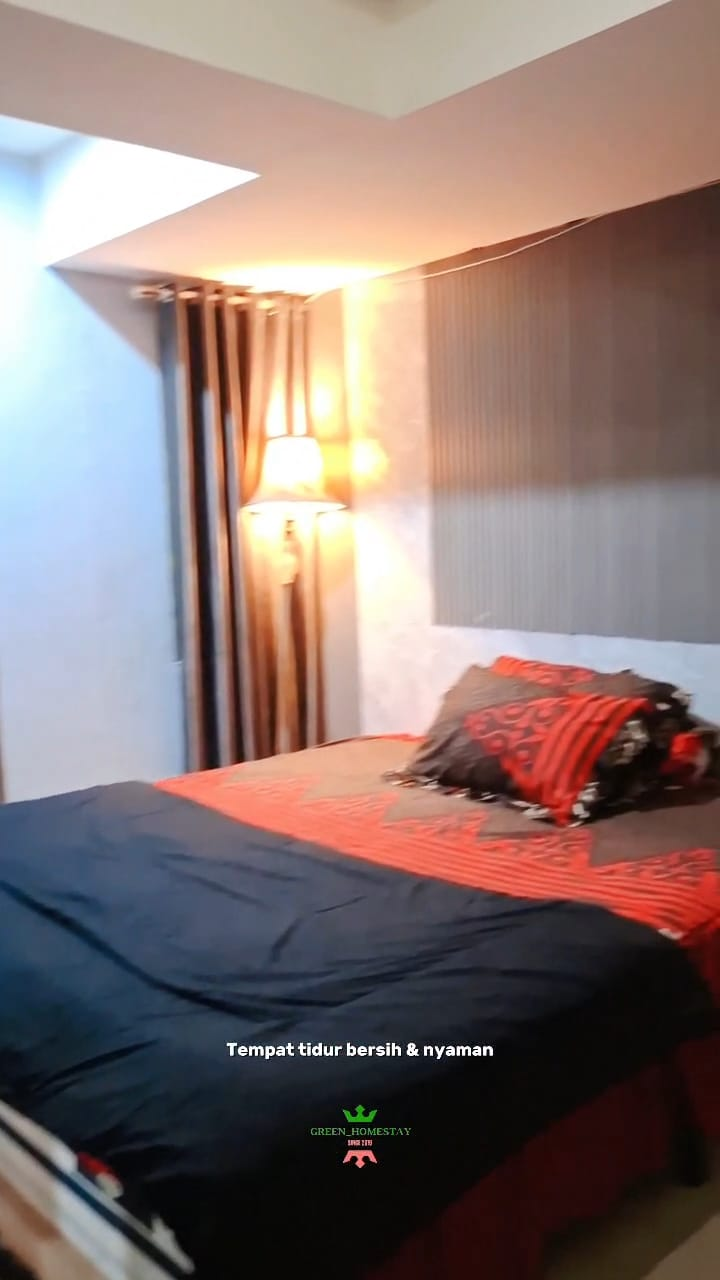
\includegraphics[width=\linewidth, max height=0.3\textheight]{Gambar/tempat tidur - studio.jpg}
                \caption{Contoh Kamar Tidur untuk Tipe Studio}
                \label{fig:tempat tidur - studio}
            \end{minipage}
            \hfill
            % Baris 1, Gambar 2 (Kanan)
            \begin{minipage}[t]{0.48\textwidth}
                \centering
                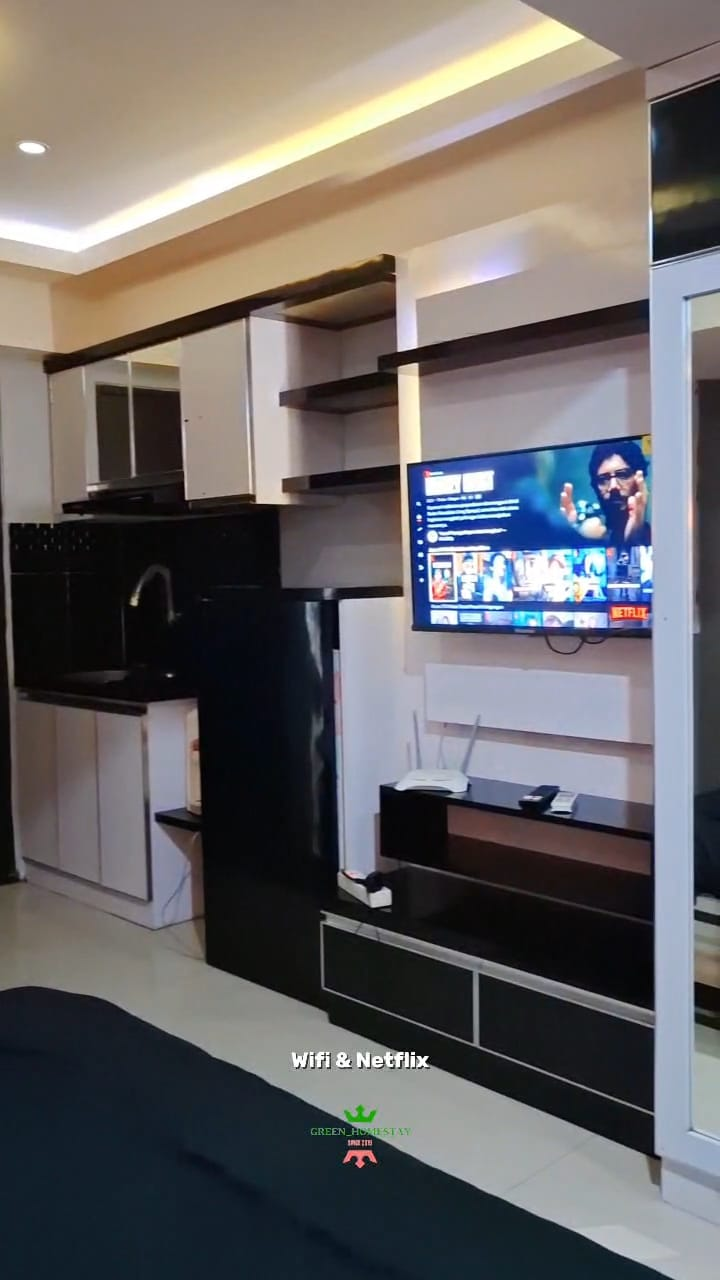
\includegraphics[width=\linewidth, max height=0.3\textheight]{Gambar/ruang tamu - studio.jpg}
                \caption{Contoh Ruang Tamu untuk Tipe Studio}
                \label{fig:ruang tamu - studio}
            \end{minipage}
        
            \vspace{1cm} % Jarak antar baris
        
            % Baris 2, Gambar 3 (Kiri)
            \begin{minipage}[t]{0.48\textwidth}
                \centering
                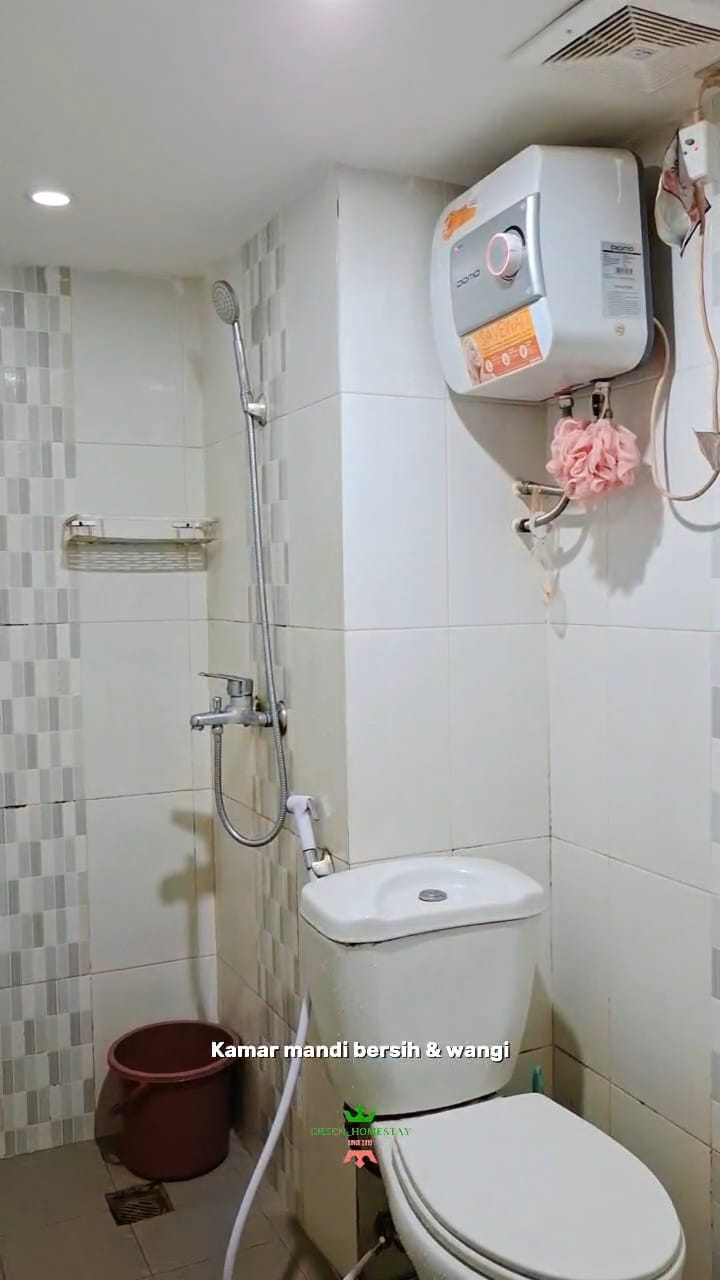
\includegraphics[width=\linewidth, max height=0.3\textheight]{Gambar/kamar mandi - studio.jpg}
                \caption{Contoh Kamar Mandi untuk Tipe Studio}
                \label{fig:kamar mandi - studio}
            \end{minipage}
            \hfill
            % Baris 2, Gambar 4 (Kanan)
            \begin{minipage}[t]{0.48\textwidth}
                \centering
                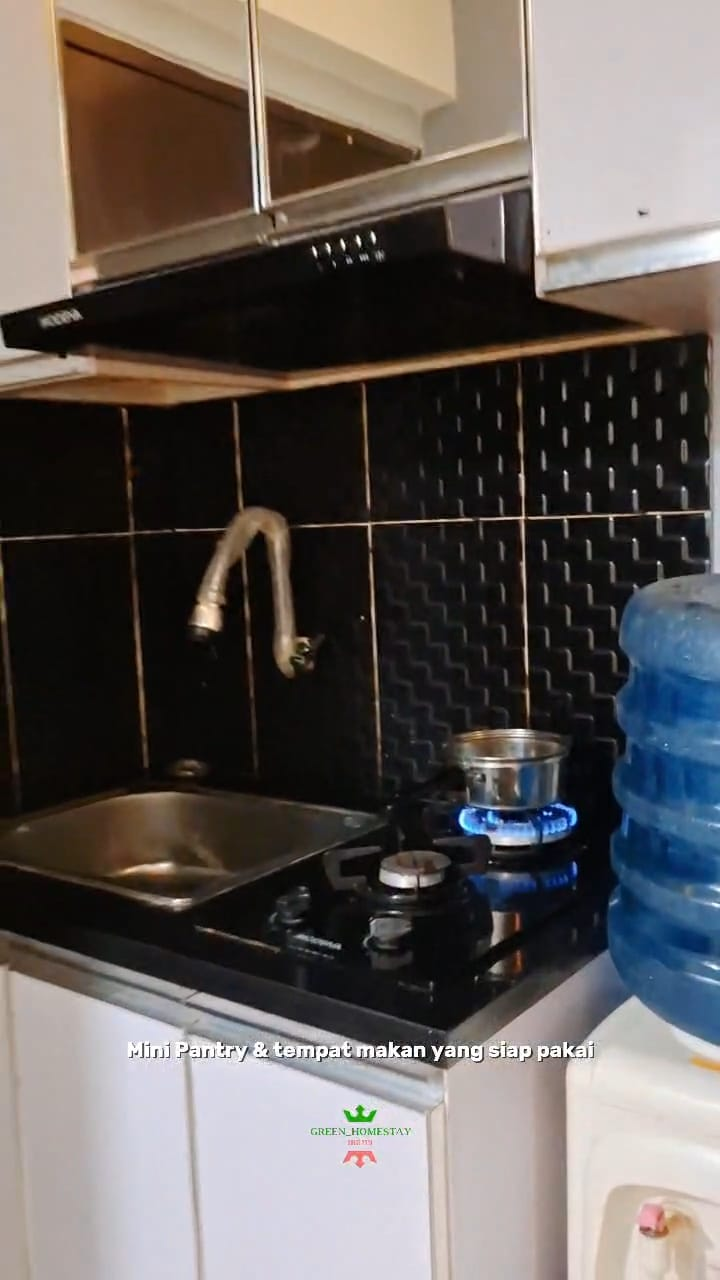
\includegraphics[width=\linewidth, max height=0.3\textheight]{Gambar/dapur - studio.jpg}
                \caption{Contoh Dapur untuk Tipe Studio}
                \label{fig:dapur - studio}
            \end{minipage}
        \end{figure}
        
        % --- GRUP 2: TIPE 2 KAMAR & AGEN (2x2) ---
        \begin{figure}[htbp]
            \centering
            % Baris 1, Gambar 1 (Kiri)
            \begin{minipage}[t]{0.48\textwidth}
                \centering
                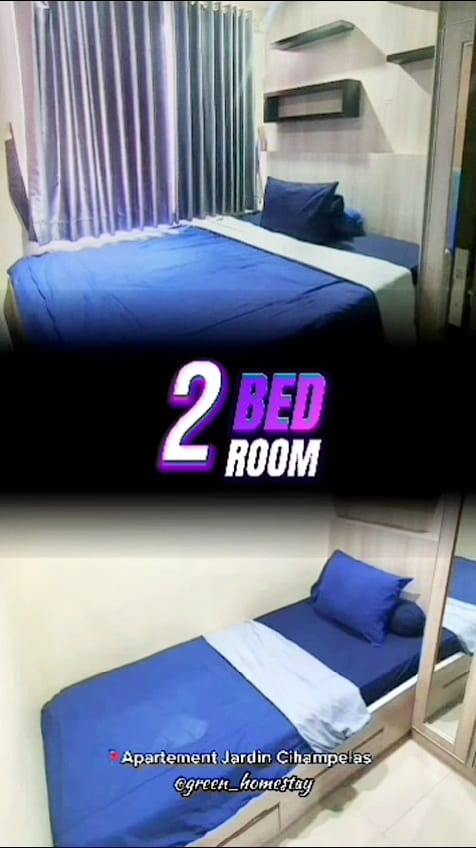
\includegraphics[width=\linewidth, max height=0.3\textheight]{Gambar/kamar - 2 kamar.jpg}
                \caption{Contoh Kamar Tidur untuk Tipe 2 Kamar}
                \label{fig:tempat tidur - 2 kamar}
            \end{minipage}
            \hfill
            % Baris 1, Gambar 2 (Kanan)
            \begin{minipage}[t]{0.48\textwidth}
                \centering
                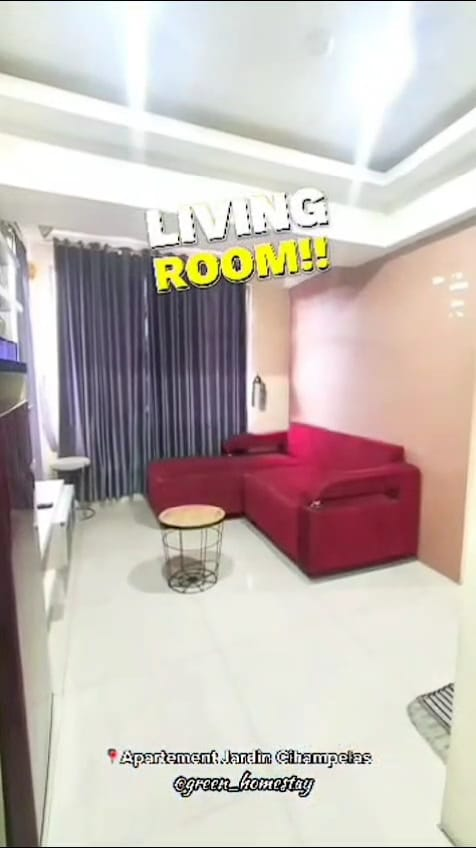
\includegraphics[width=\linewidth, max height=0.3\textheight]{Gambar/ruang tamu - 2 kamar.jpg}
                \caption{Contoh Ruang Tamu untuk Tipe 2 Kamar}
                \label{fig:ruang tamu - 2 kamar}
            \end{minipage}
        
            \vspace{1cm} % Jarak antar baris
        
            % Baris 2, Gambar 3 (Kiri)
            \begin{minipage}[t]{0.48\textwidth}
                \centering
                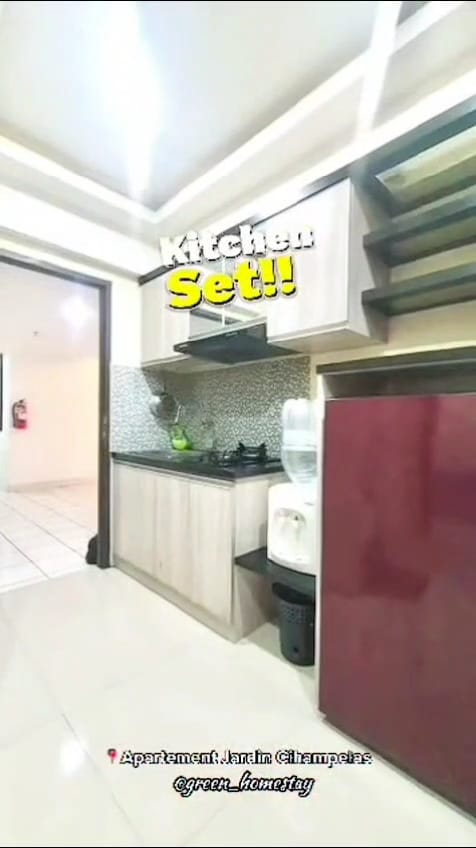
\includegraphics[width=\linewidth, max height=0.3\textheight]{Gambar/dapur - 2 kamar.jpg}
                \caption{Contoh Dapur untuk Tipe 2 Kamar}
                \label{fig:dapur - 2 kamar}
            \end{minipage}
            \hfill
            % Baris 2, Gambar 4 (Kanan)
            \begin{minipage}[t]{0.48\textwidth}
                \centering
                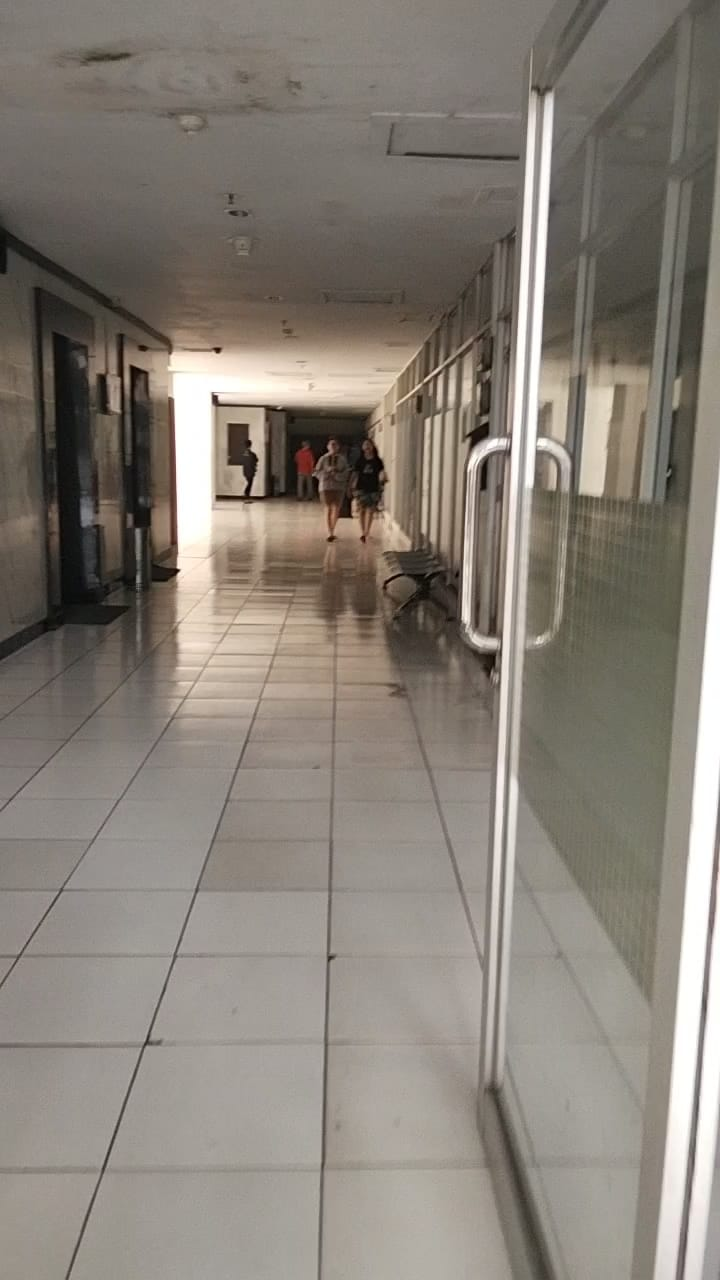
\includegraphics[width=\linewidth, max height=0.3\textheight]{Gambar/tampak depan ruangan2 agen.jpg}
                \caption{Lorong Tempat Ruangan Para Pelaku Komersil}
                \label{fig:tampak depan ruangan2 agen}
            \end{minipage}
        \end{figure}
        

        \begin{figure}[H]
            \centering
            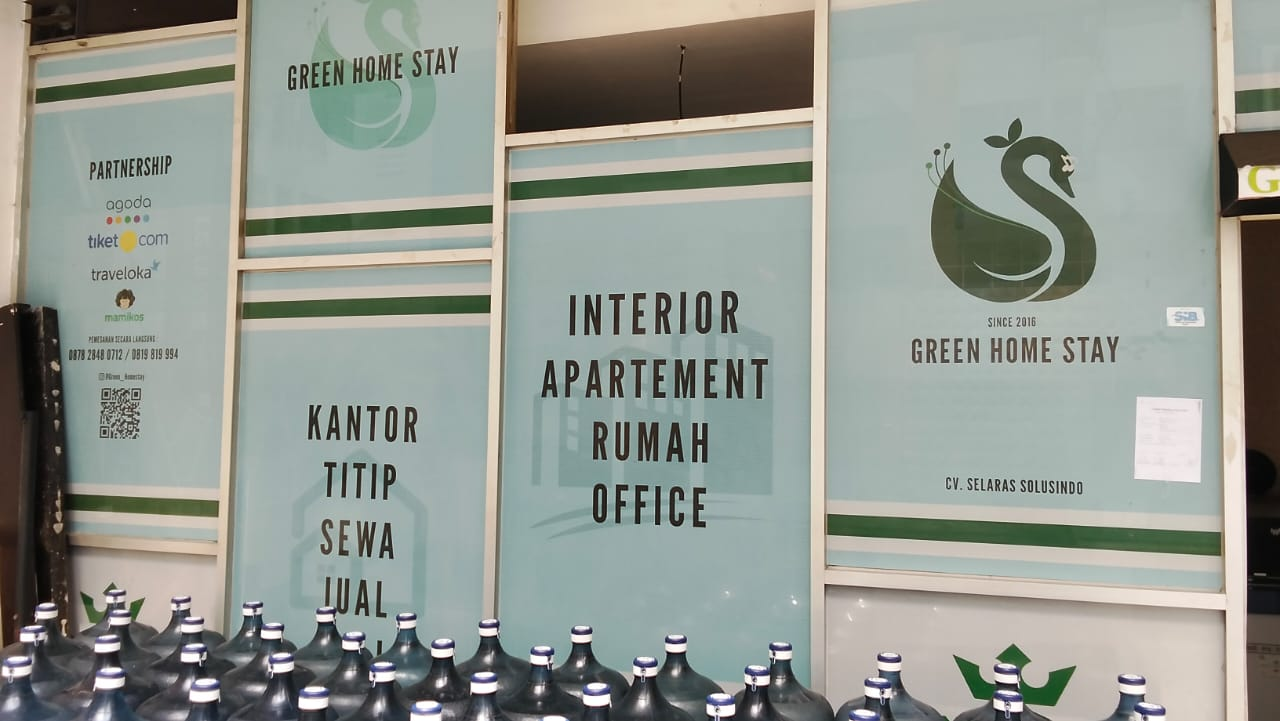
\includegraphics[width=0.6\textwidth, max height=0.25\textheight]{Gambar/ruang salah 1 agen.jpg}
            \caption{Salah Satu Ruang Pelaku Komersil}
            \label{fig:ruang salah 1 agen}
        \end{figure}

        
        Tempat parkir B1 diprioritaskan untuk para pemilik unit, pengurus, dan sepeda; sedangkan tempat parkir B2 diprioritaskan untuk para penyewa; dan tempat parkir B3 untuk sepeda motor.
        
        \vspace{1cm}
        \begin{figure}[H]
            \centering
            \begin{minipage}[b]{0.48\textwidth}
                \centering
                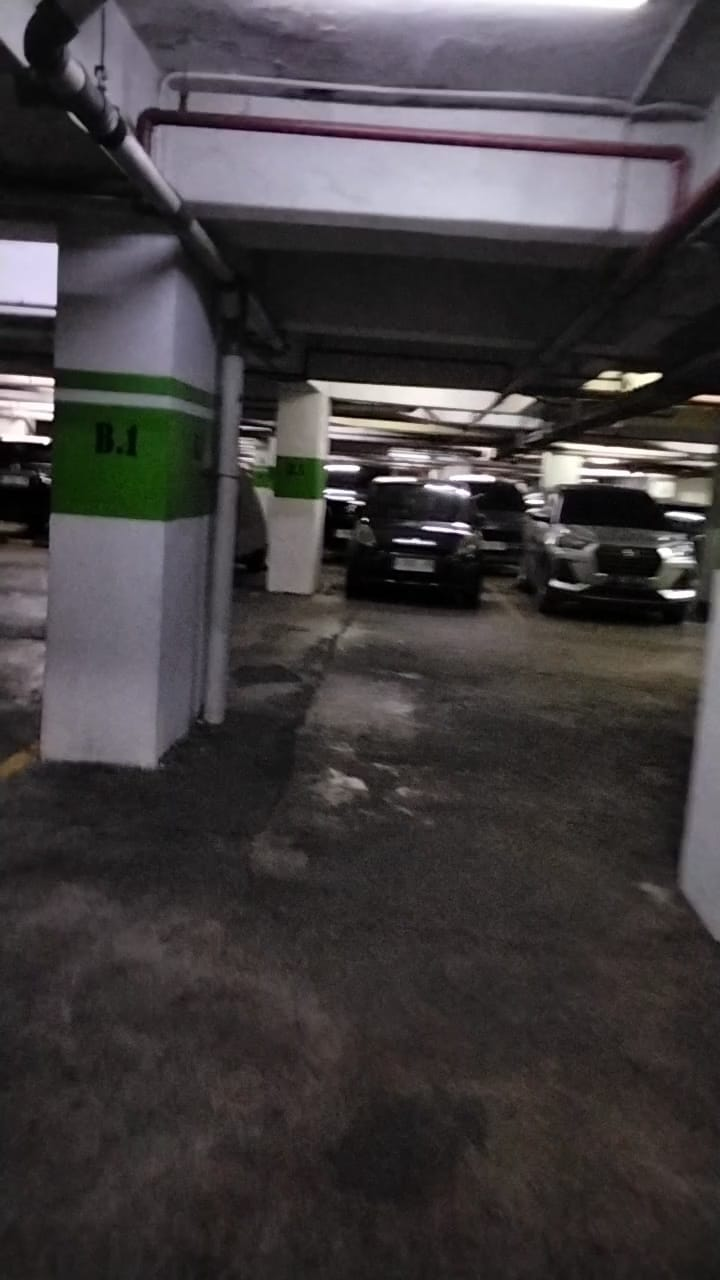
\includegraphics[width=\textwidth, max height=0.25\textheight, keepaspectratio]{Gambar/parkir b1.jpg}
                \caption{Tempat Parkir B1}
                \label{fig:b1}
            \end{minipage}
            \hfill
            \begin{minipage}[b]{0.48\textwidth}
                \centering
                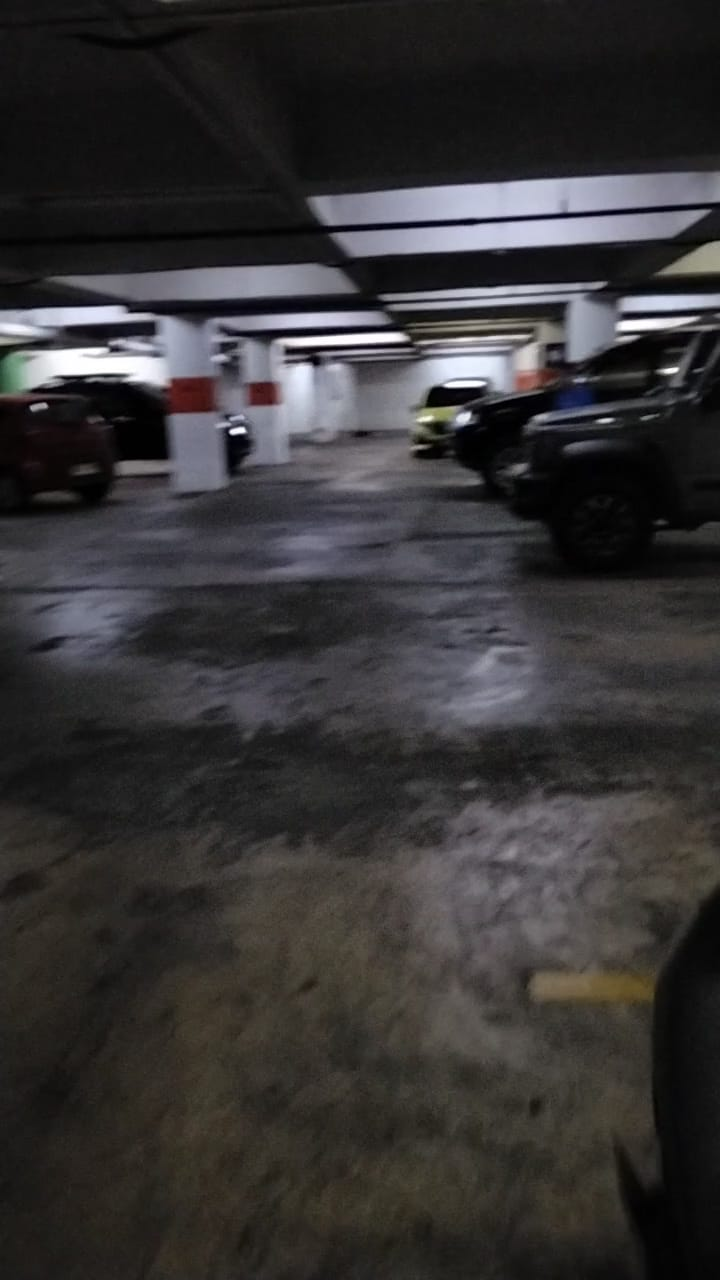
\includegraphics[width=\textwidth, max height=0.25\textheight, keepaspectratio]{Gambar/parkir b2.jpg}
                \caption{Tempat Parkir B2}
                \label{fig:b2_1}
            \end{minipage}
        \end{figure}
        

        % \newpage
        \noindent\begin{minipage}{\textwidth}
        Ruang Badan Pengelola P3SRS berfungsi untuk mengajukan pengaduan, melakukan pembayaran parkir bulanan, dan membayar tagihan IPL.
        \begin{figure}[H]
            \centering
            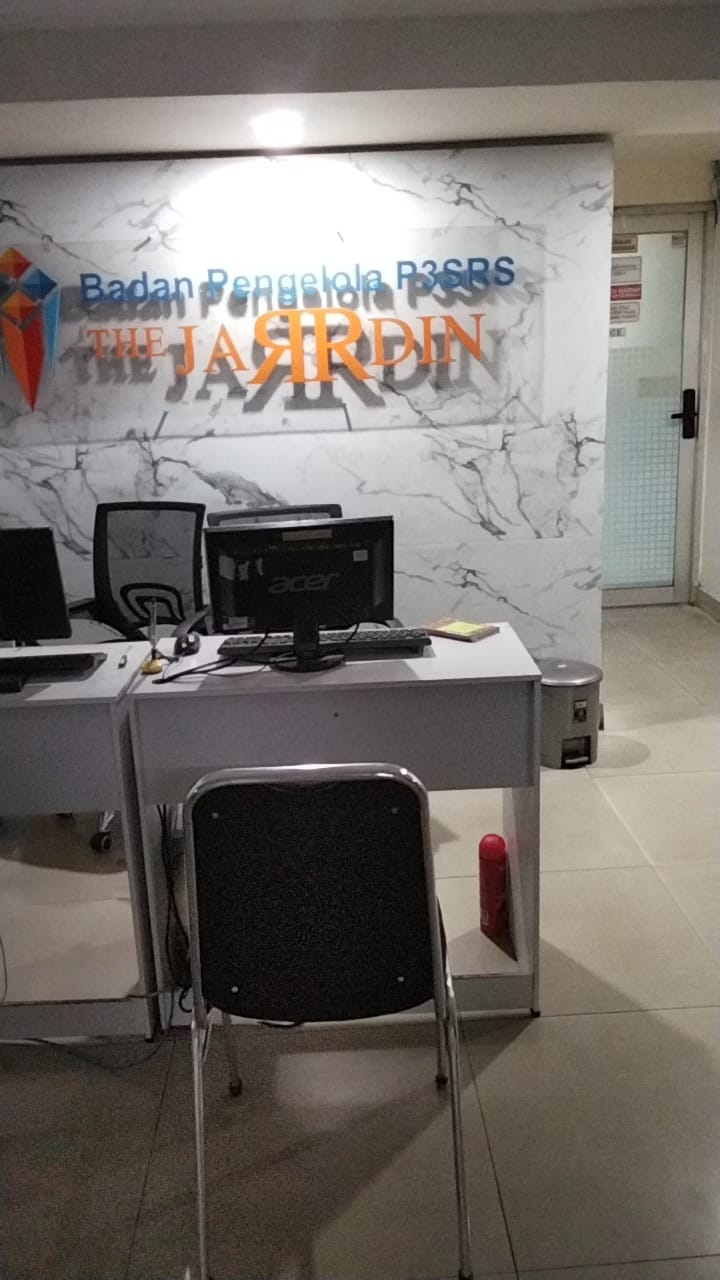
\includegraphics[width=0.6\textwidth, max height=0.25\textheight]{Gambar/ruang badan pengelola p3srs.jpg}
            \caption{Ruang Badan Pengelola P3SRS}
            \label{fig:b2_2}
        \end{figure}
        \end{minipage}
        % \vspace{0.5cm}


        Berikut adalah ruangan-ruangan untuk keamanan dan pemeliharaan lingkungan Rusunami The Jarrdin.
        \begin{figure}[H]
            \centering
            \begin{minipage}[b]{0.48\textwidth}
                \centering
                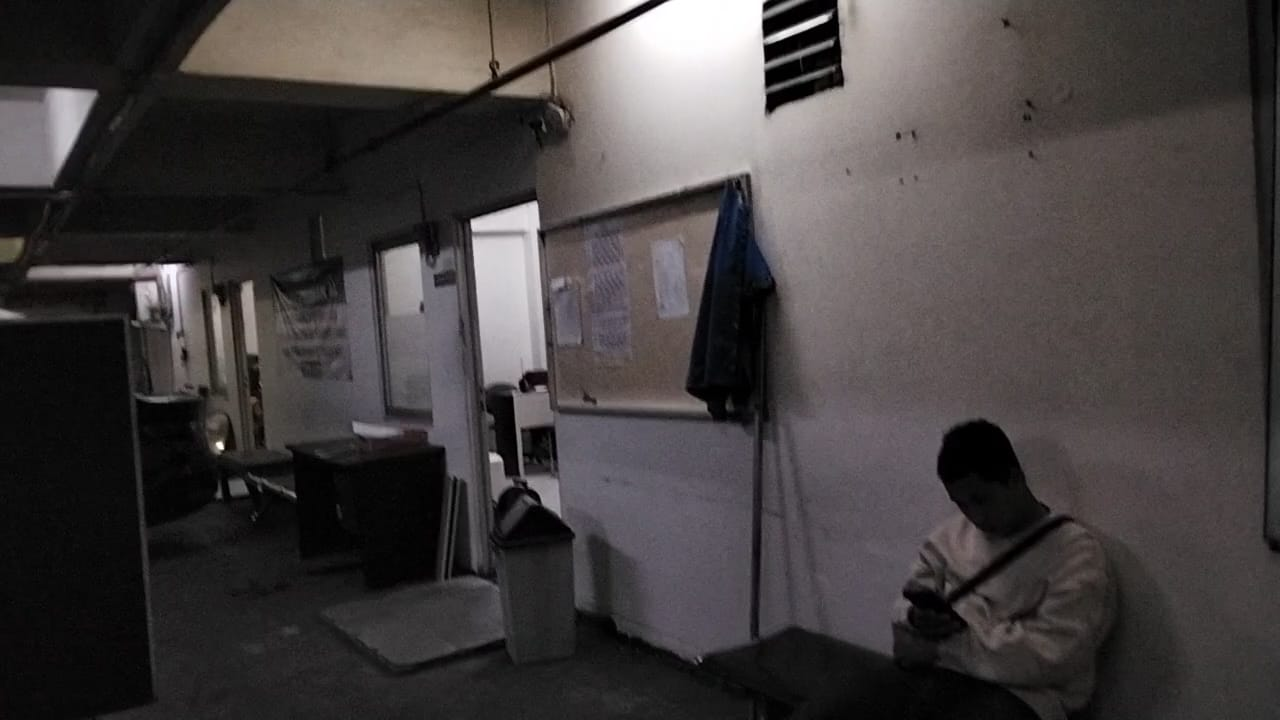
\includegraphics[width=\textwidth, max height=0.25\textheight, keepaspectratio]{Gambar/ruangan-ruangan untuk para pemelihara.jpg}
                \caption{Ruangan-Ruangan Pemelihara}
                \label{fig:ruang pemelihara}
            \end{minipage}
            \hfill
            \begin{minipage}[b]{0.48\textwidth}
                \centering
                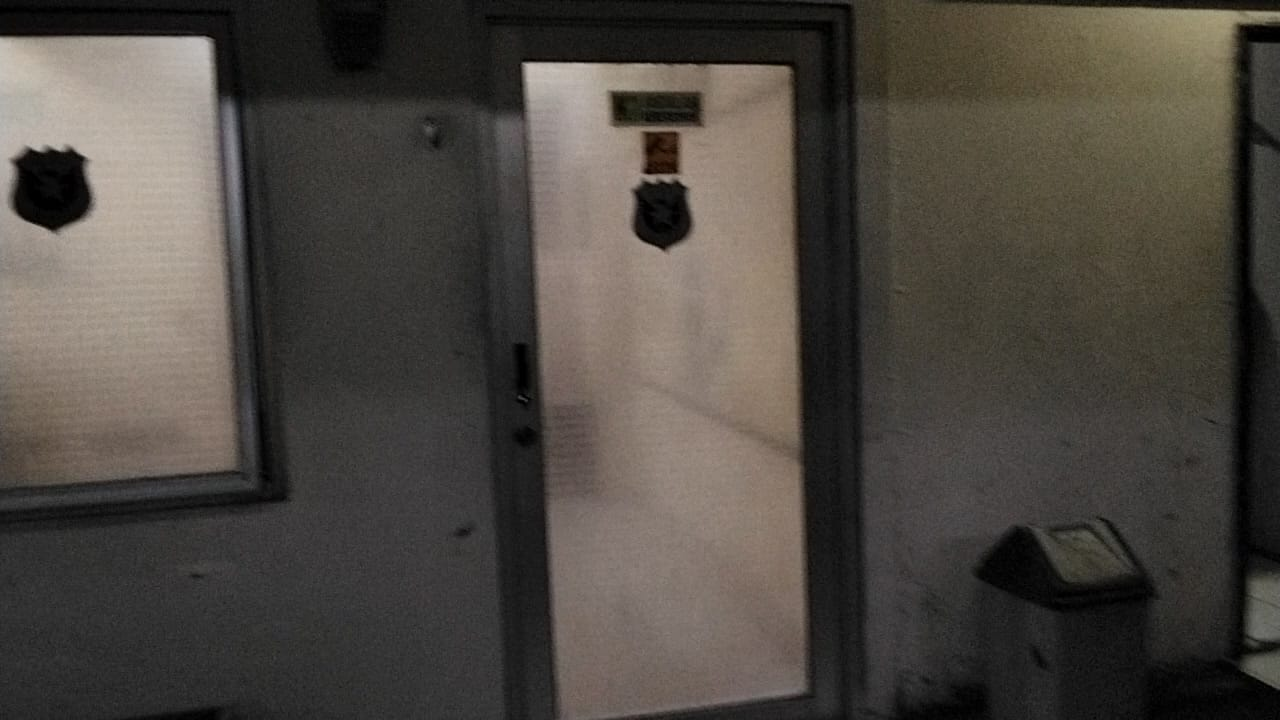
\includegraphics[width=\textwidth, max height=0.25\textheight, keepaspectratio]{Gambar/ruang security.jpg}
                \caption{Ruangan Keamanan}
                \label{fig:ruang security}
            \end{minipage}
            
            \vspace{0.5cm}
            \begin{minipage}[b]{0.48\textwidth}
                \centering
                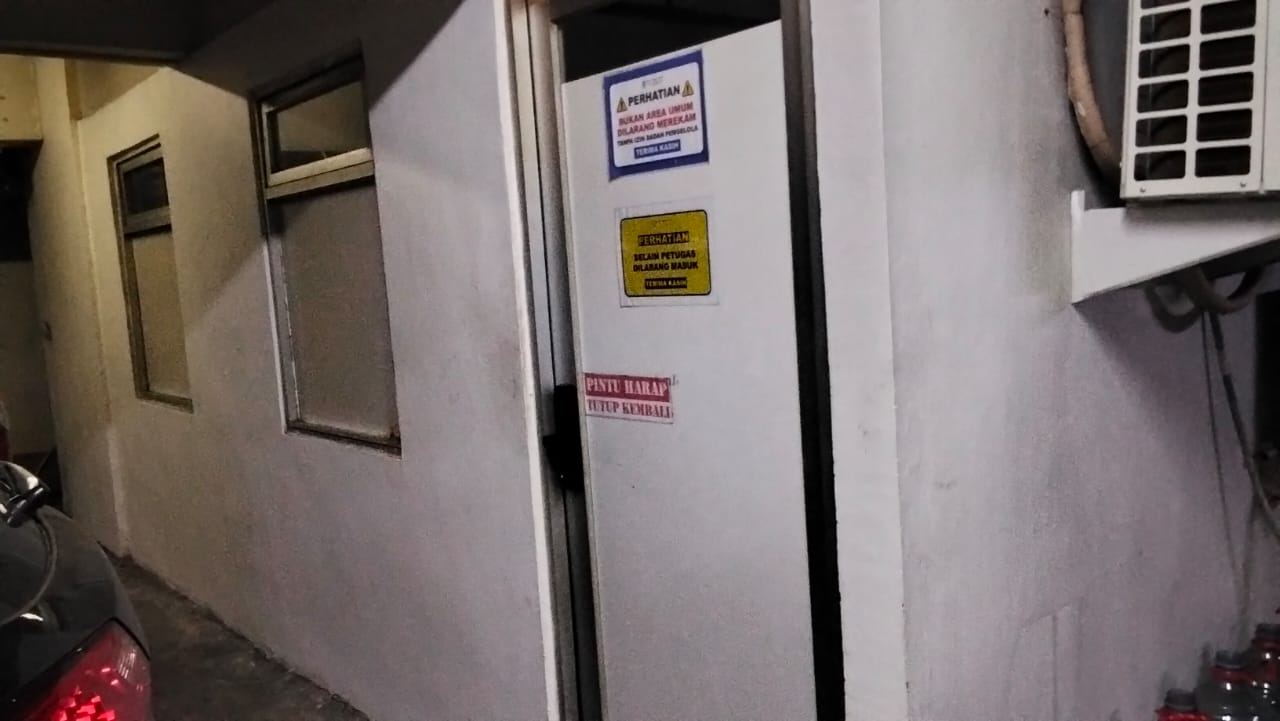
\includegraphics[width=\textwidth, max height=0.25\textheight, keepaspectratio]{Gambar/ruang cctv.jpg}
                \caption{Ruangan CCTV}
                \label{fig:ruang cctv}
            \end{minipage}
            \hfill
            \begin{minipage}[b]{0.48\textwidth}
                \centering
                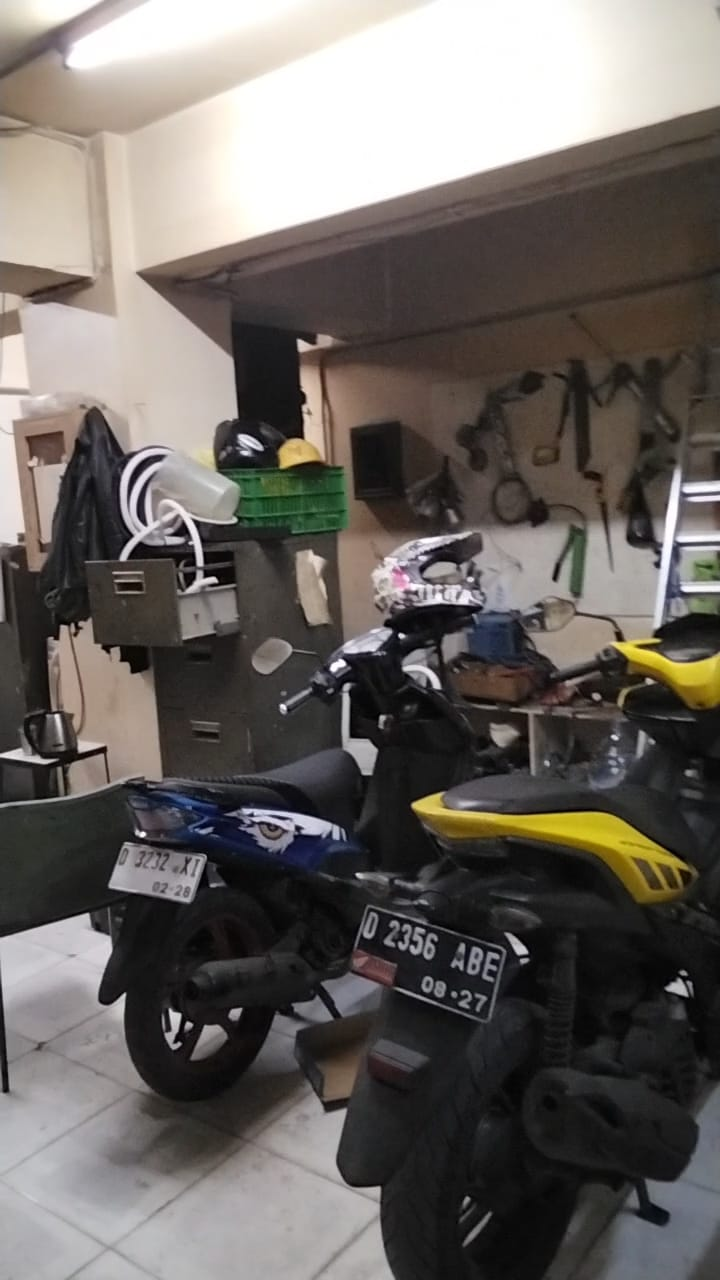
\includegraphics[width=\textwidth, max height=0.25\textheight, keepaspectratio]{Gambar/ruang engineering.jpg}
                \caption{Ruangan {\it Engineering}}
                \label{fig:ruang engineering}
            \end{minipage}
        \end{figure}

        Berikut contoh fasilitas yang disediakan oleh Rusunami The Jarrdin.
        \begin{figure}[H]
            \centering
            \begin{minipage}[b]{0.48\textwidth}
                \centering
                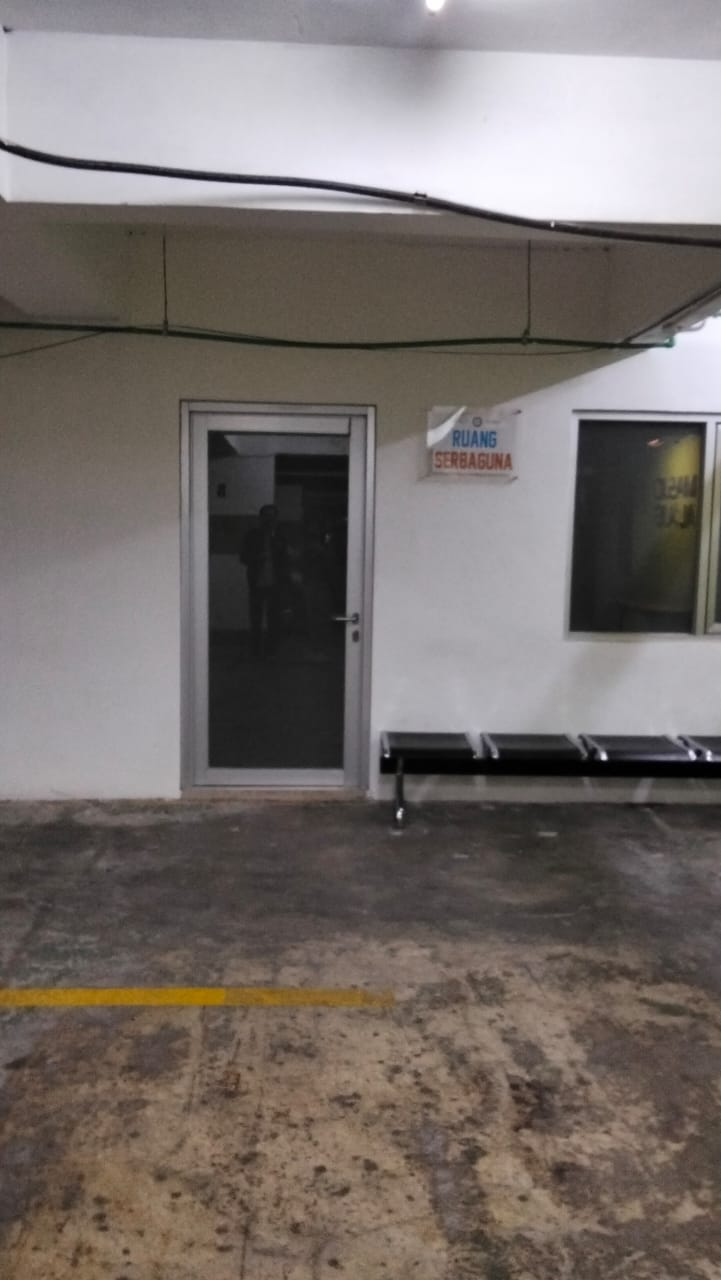
\includegraphics[width=\textwidth, max height=0.25\textheight, keepaspectratio]{Gambar/fasilitas ruang serbaguna.jpg}
                \caption{Fasilitas Ruang Serbaguna}
                \label{fig:fasilitas ruang serbaguna}
            \end{minipage}
            \hfill
            \begin{minipage}[b]{0.48\textwidth}
                \centering
                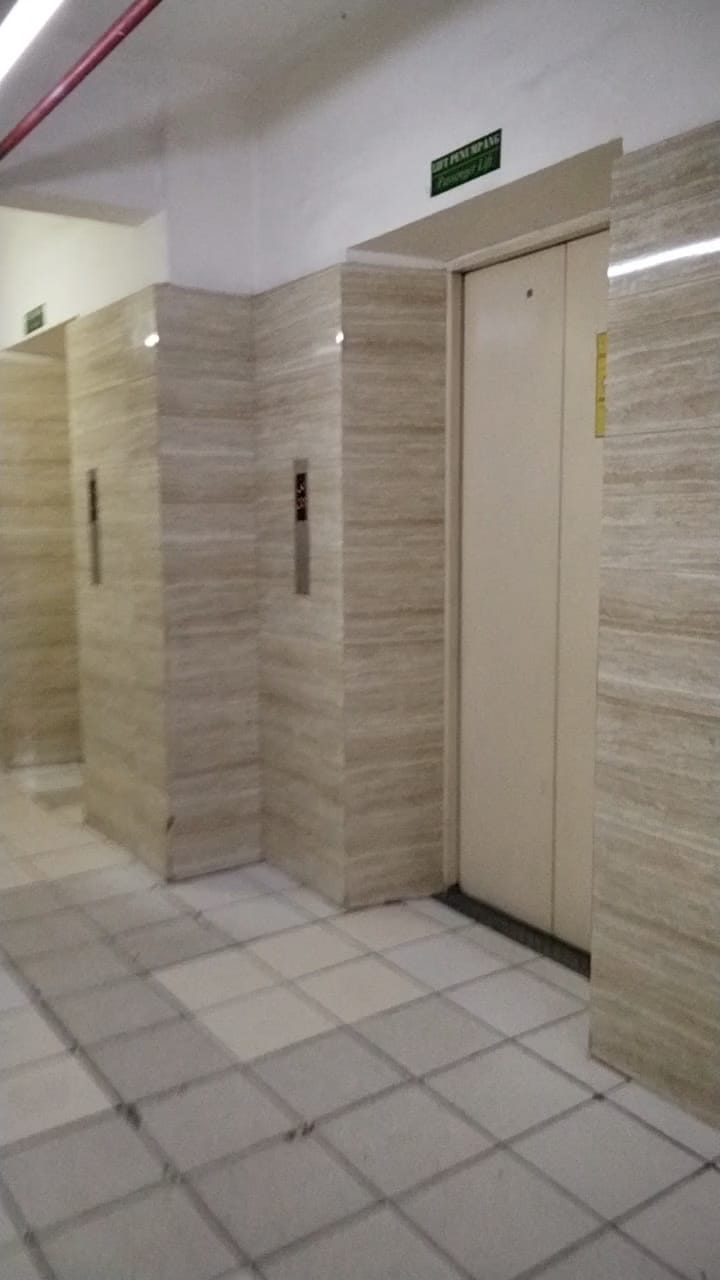
\includegraphics[width=\textwidth, max height=0.25\textheight, keepaspectratio]{Gambar/lift.jpg}
                \caption{Fasilitas Lift}
                \label{fig:lift}
            \end{minipage}
        \end{figure}

        \begin{figure}[H]
            \centering
            \begin{minipage}[b]{0.48\textwidth}
                \centering
                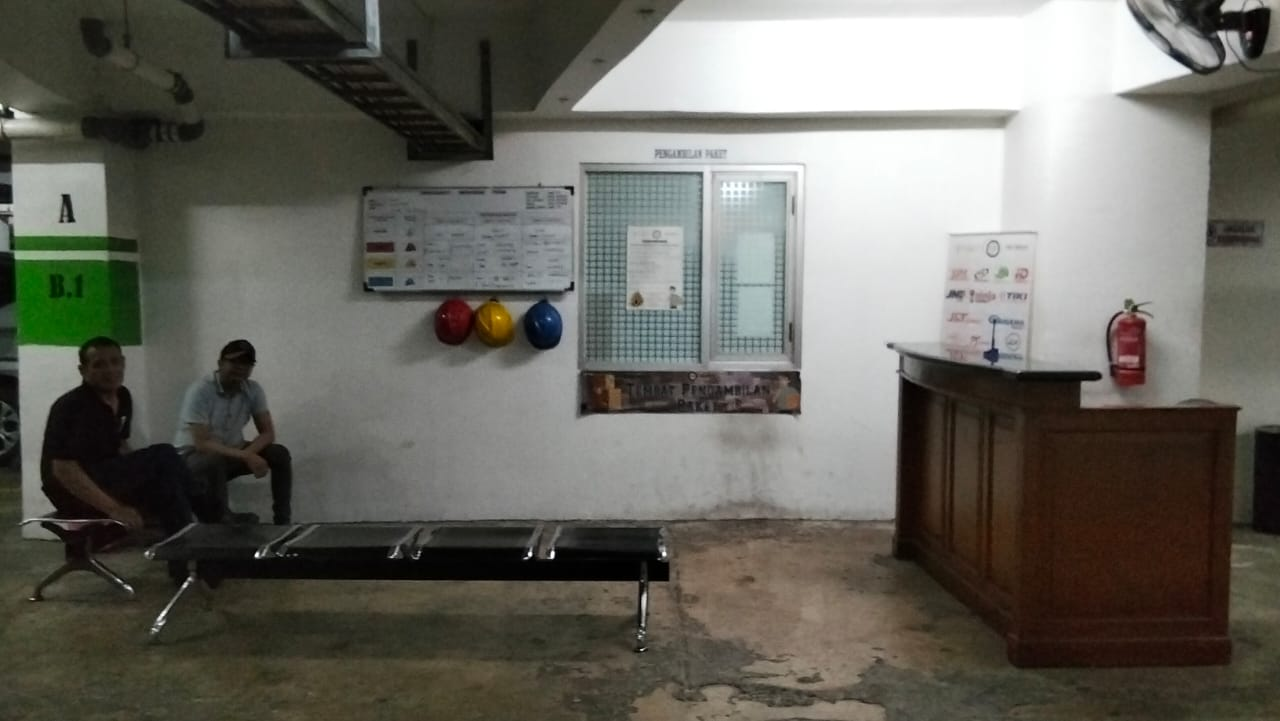
\includegraphics[width=\textwidth, max height=0.3\textheight, keepaspectratio]{Gambar/tempat ambil paket.jpg}
                \caption{Fasilitas Tempat Ambil Paket}
                \label{fig:tempat ambil paket}
            \end{minipage}
            \hfill
            \begin{minipage}[b]{0.48\textwidth}
                \centering
                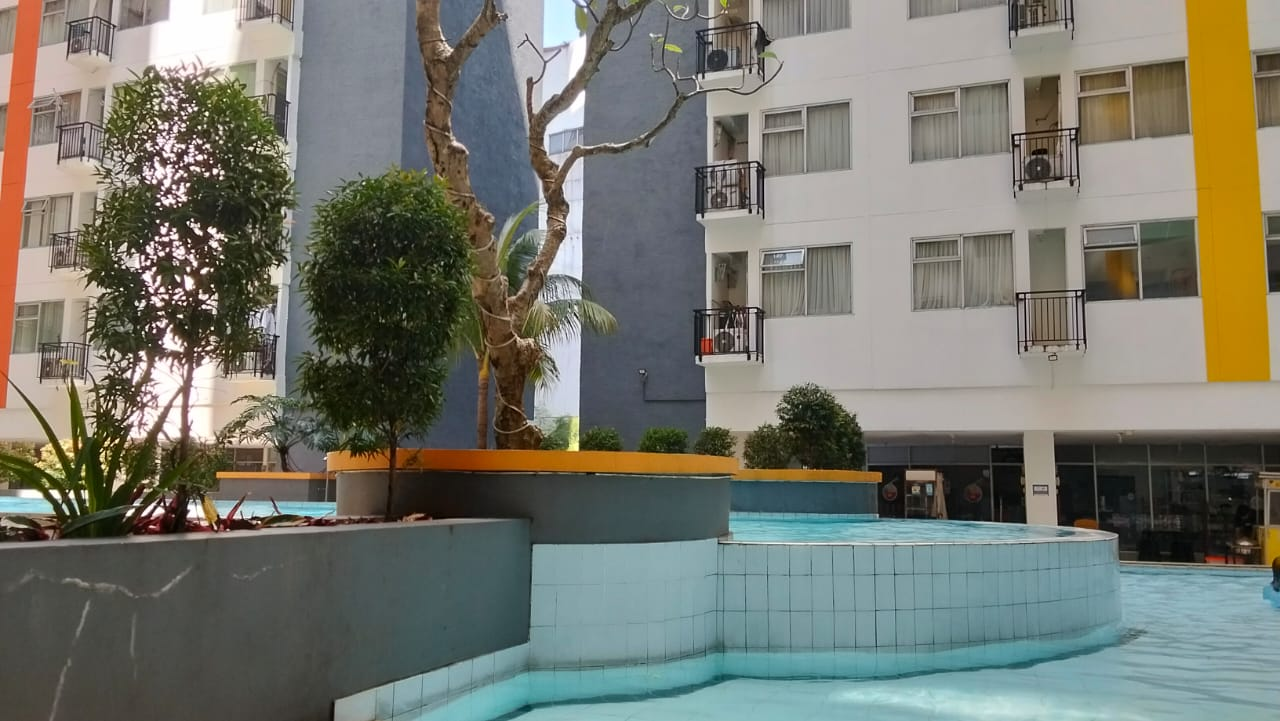
\includegraphics[width=\textwidth, max height=0.3\textheight, keepaspectratio]{Gambar/kolam renang.jpg}
                \caption{Fasilitas Kolam Renang}
                \label{fig:fasilitas kolam renang}
            \end{minipage}
        \end{figure}


        

        % \vspace{-5cm}
        Tersedianya berbagai akses keluar masuk ke kawasan The Jarrdin, seperti akses jalan untuk para pejalan kaki, tangga darurat, dan basement membuat keamanan tidak optimal.

        % \vspace{-2cm}
        \begin{figure}[H]
            \centering
            \begin{minipage}[b]{0.49\textwidth}
                \centering
                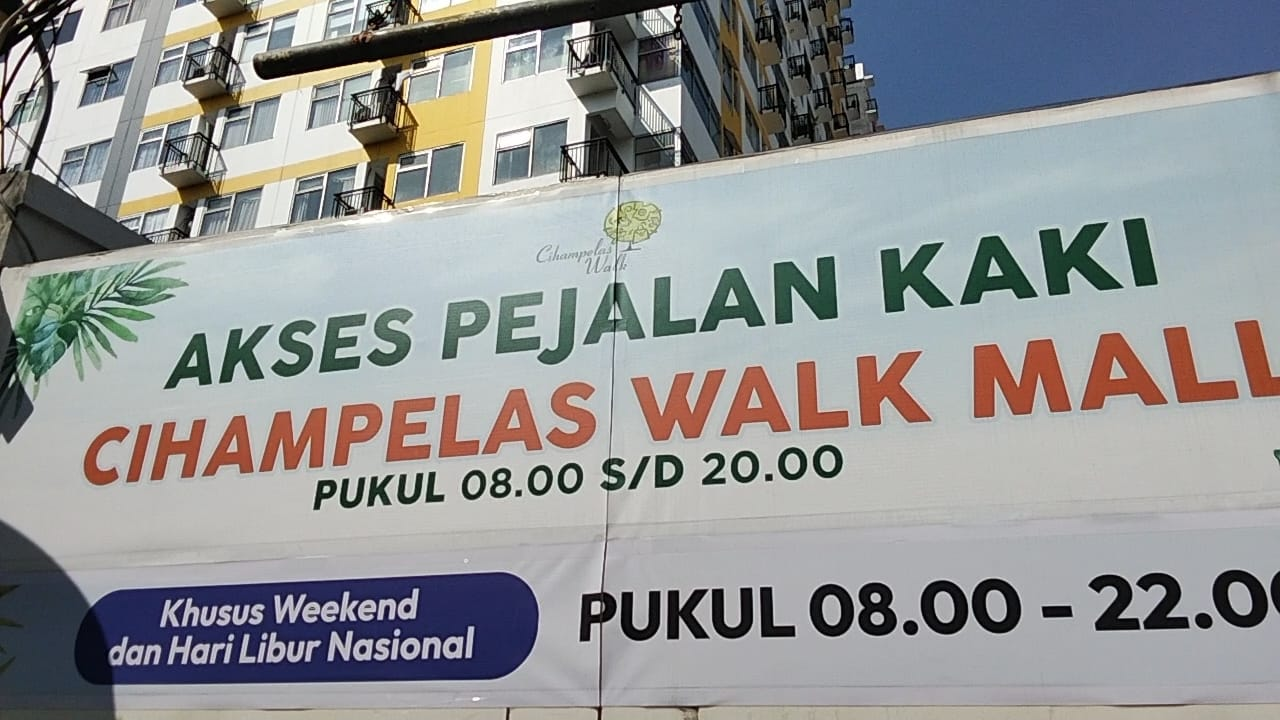
\includegraphics[width=\textwidth,max height=0.3\textheight,keepaspectratio]{Gambar/fasilitas akses ke ciwalk.jpg}
                \caption{Fasilitas Akses Jalan Menuju Ciwalk}
                \label{fig:fasilitas-akses-ciwalk}
            \end{minipage}
            \hfill
            \begin{minipage}[b]{0.49\textwidth}
                \centering
                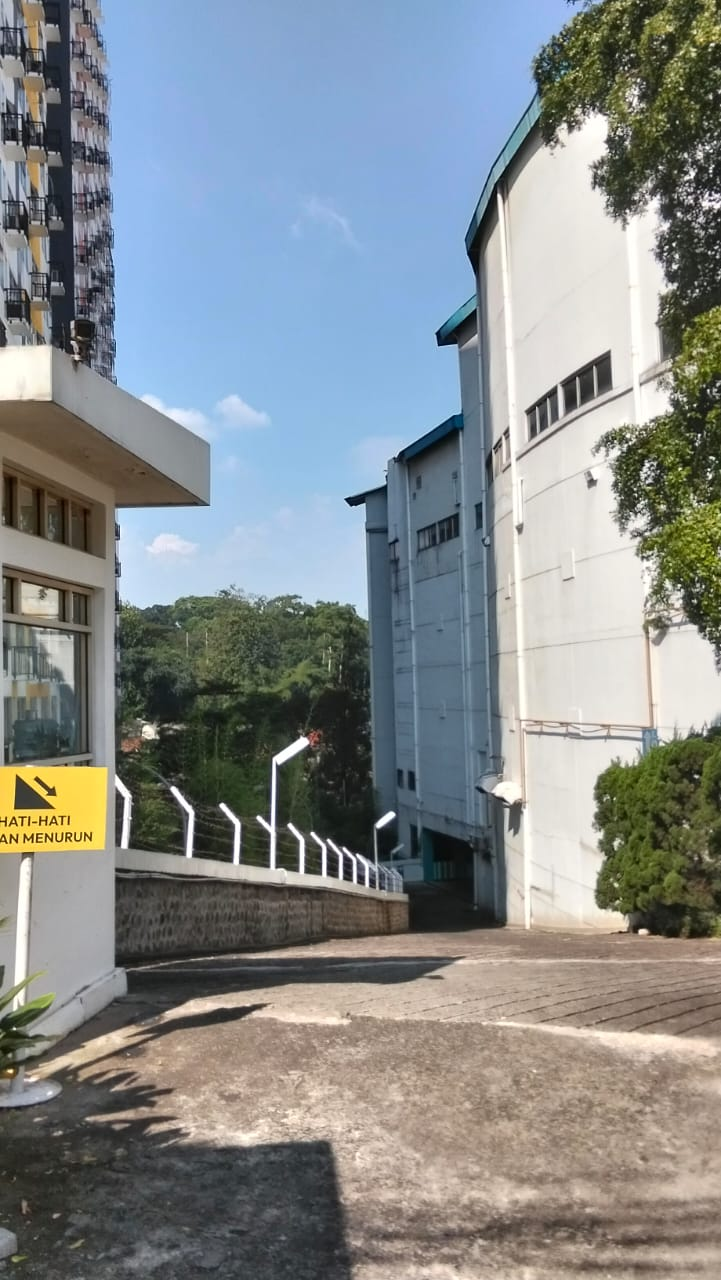
\includegraphics[width=\textwidth,max height=0.25\textheight,keepaspectratio]{Gambar/akses jalan menuju ciwalk.jpg}
                \caption{Akses Jalan Menuju Ciwalk}
                \label{fig:akses-jalan-ciwalk}
            \end{minipage}
        \end{figure}
        
        \begin{figure}[H]
            \centering
            % --- Gambar Kiri ---
            \begin{minipage}[t]{0.48\textwidth}
                \centering
                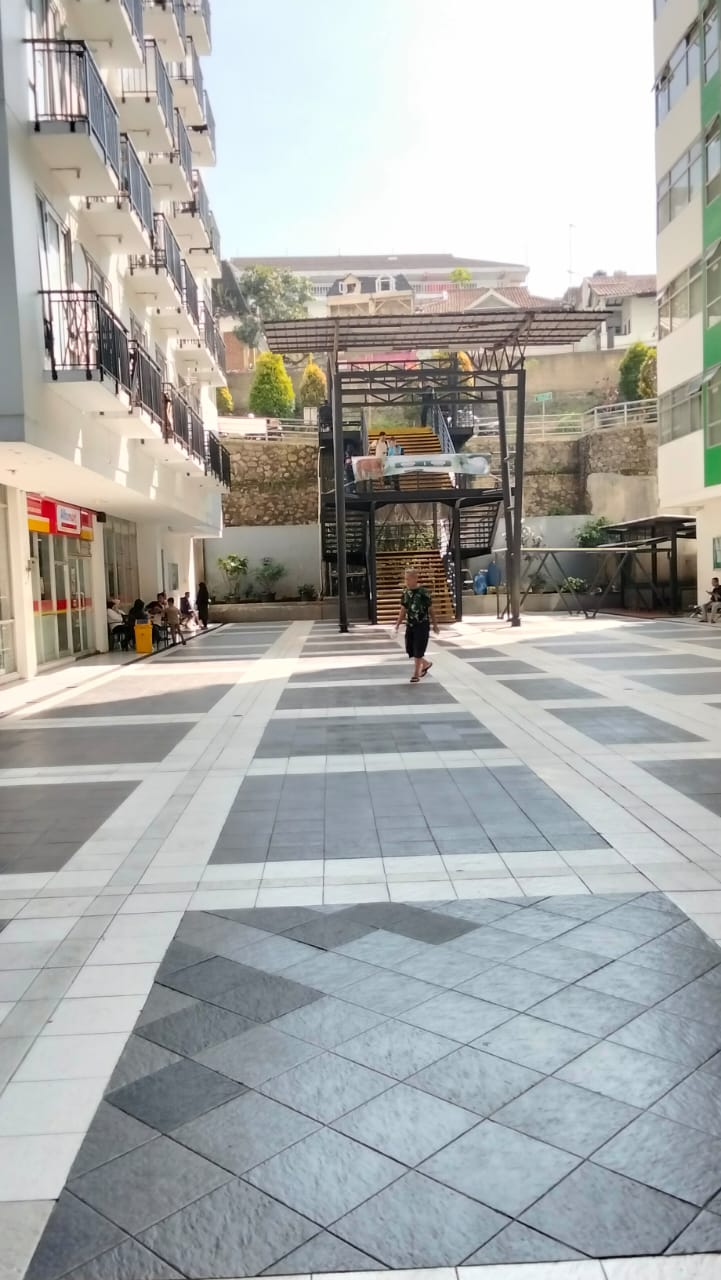
\includegraphics[width=\linewidth, max height=0.25\textheight]{Gambar/akses tangga untuk pejalan kaki.jpg}
                \caption{Fasilitas Akses Tangga untuk Pejalan Kaki}
                \label{fig:akses tangga untuk pejalan kaki}
            \end{minipage}
            \hfill
            % --- Gambar Kanan ---
            \begin{minipage}[t]{0.48\textwidth}
                \centering
                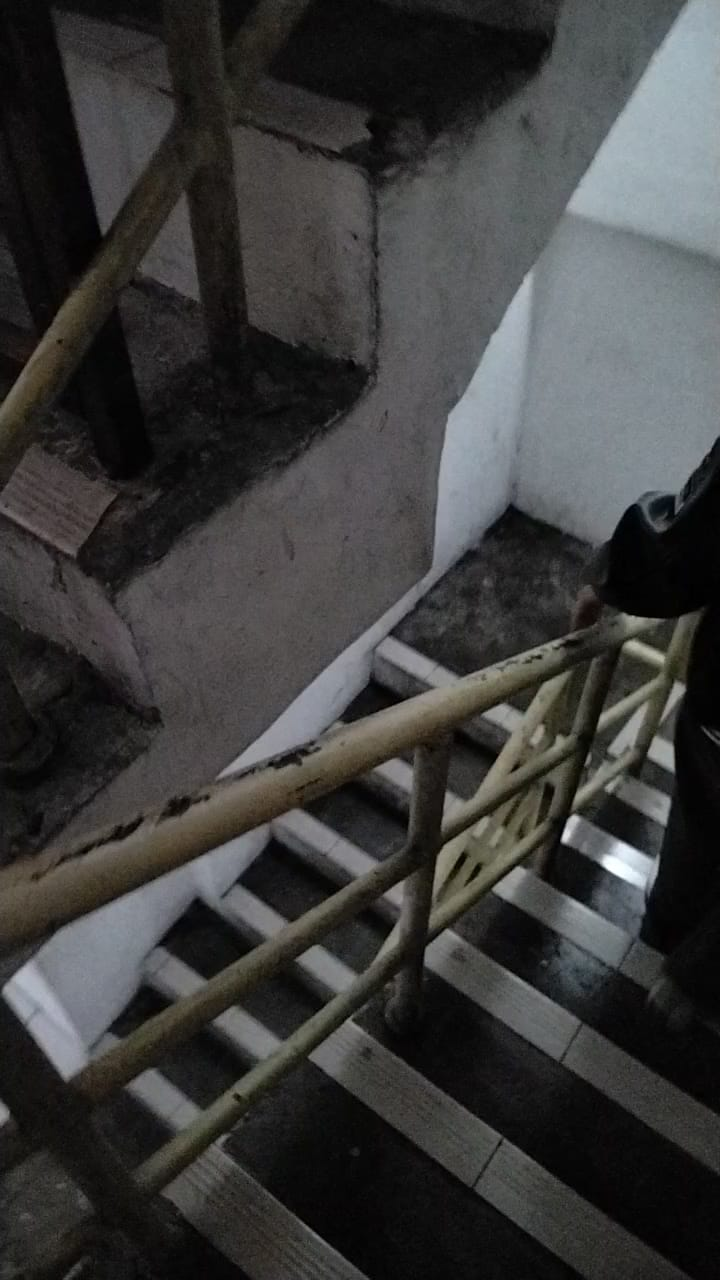
\includegraphics[width=\linewidth, max height=0.25\textheight]{Gambar/tangga darurat.jpg}
                \caption{Fasilitas Tangga Darurat}
                \label{fig:tangga darurat}
            \end{minipage}
        \end{figure}
        

\newpage
\subsection{Kebutuhan Fungsional Sistem}
Berdasarkan hasil analisis masalah dan masukan dari narasumber, sistem yang akan dibangun harus memenuhi kebutuhan fungsional sebagai berikut.

\begin{enumerate}
    \item \textbf{Manajemen data terpusat dengan kontrol akses berjenjang}\\
    Sistem harus memfasilitasi input data oleh pelaku komersil, namun membatasi akses data sesuai peran. Pelaku komersil hanya dapat melihat data kelolaannya sendiri, sementara pihak pengelola (Ketua Agen, P3SRS, atau PKJ) memiliki akses global untuk pengawasan dan deteksi duplikasi penyewa antar-pelaku komersil.
    
    \item \textbf{Master data unit}\\
    Untuk meminimalisir kesalahan input manual dan mempercepat proses, sistem perlu menyediakan \textit{master data} unit. Pelaku komersil cukup memilih unit dari daftar yang tersedia yang telah dipetakan sesuai hak kelola mereka.
    
    \item \textbf{Pencatatan riwayat dan log aktivitas}\\
    Setiap perubahan data (seperti perpanjangan sewa, pengeditan metode bayar, atau perubahan status check-out) harus tercatat dalam \textit{log history} yang tidak dapat dihapus. Fitur ini krusial untuk audit jejak digital apabila terjadi sengketa atau investigasi pelanggaran.
    
    \item \textbf{Pelaporan pelanggaran visual}\\
    Sistem harus mendukung unggahan bukti foto pelanggaran yang ditampilkan pada \textit{dashboard} sebagai rekam jejak digital. Selain untuk mendokumentasikan pelanggaran fisik (seperti kerusakan unit, temuan barang terlarang, atau kondisi unit yang tidak layak), penayangan bukti visual ini juga bertujuan memberikan efek jera bagi para pelanggar.
    
    \item \textbf{Deteksi profil risiko penyewa}\\
    Sistem perlu memiliki fitur untuk mendeteksi nama atau NIK penyewa yang muncul berulang kali di berbagai pelaku komersil yang berbeda (\textit{hopping}), yang bisa menjadi indikator perilaku mencurigakan.
\end{enumerate}
